\documentclass[manuscript,screen,review]{acmart}

%% ===================== 中文支持 =====================
%% 本文为中文稿,必须用 XeLaTeX 编译(pdfLaTeX 无法处理中文)。
%% scheme=plain 让 ctex 只接管中文字体与断行,不改写 acmart 的标题版式与章节名,
%% 否则两者会争夺 \section 的定义而报错。
%% fontset=windows 使用系统的宋体/黑体;若改到 Linux 或 Overleaf 上编译,
%% 把它换成 fontset=fandol(TeX Live 自带,无需系统字体)。
\usepackage[UTF8,scheme=plain,fontset=windows]{ctex}

\usepackage{algorithm}
% Use algorithmicx + algpseudocode: provides \Require, \Ensure, \State, and \Comment
\usepackage{algorithmicx}
\usepackage{algpseudocode}
\usepackage{tikz}
% Load common tikz libraries used in figures (positioning provides the "of" syntax)
\usetikzlibrary{positioning,arrows.meta,calc,shapes,shadows}
% color support for \textcolor used inside algorithms
\usepackage{xcolor}
% Math packages required for \text and bold symbols inside math
\usepackage{amsmath}
\usepackage{bm}
\usepackage{multirow}
% Enable list customization (leftmargin, itemsep, etc.) used in the document
\usepackage{enumitem}
% Ensure header height is sufficient for fancyhdr
\setlength{\headheight}{20.48303pt}
% Visible placeholder for numbers still awaiting the controlled matrix run.
% Every occurrence must be gone before submission: grep for \TBD.
\newcommand{\TBD}[1]{\textcolor{red}{\textbf{[TBD:} #1\textbf{]}}}
% theorem environments used in the document
\usepackage{amsthm}
\newtheorem{assumption}{假设}
\newtheorem{problem}{问题}
% Define remark environment (was missing and caused compilation errors)
\newtheorem{remark}{注}
% acmart 自己已经定义了 proposition 与 lemma(英文名),不能用 \newtheorem 重名覆盖,
% 也没有提供改名接口,故另起两个中文环境,正文用 prop / lem。
\newtheorem{prop}{命题}
\newtheorem{lem}{引理}

%% 浮动体与交叉引用的中文名称。ctex 用 scheme=plain 载入时不会改这些,须手工设定。
\renewcommand{\figurename}{图}
\renewcommand{\tablename}{表}
\floatname{algorithm}{算法}
\renewcommand{\proofname}{证明}

%% ===================== 全文图表的重建顺序 =====================
%% 有先后依赖,按序执行。前两步在 clbs/ 目录下跑,后两步在仓库根目录跑。
%%
%%  1. 主结果(约 6 小时,决定下面所有数字):
%%       py -u -m tools.baseline_ladder --budget 90 \
%%          --seeds 42,7,2024,13,1,99,123,777,31415,8      -> output/baseline_ladder.csv
%%  2. 三个配套批次(可在 1 之后依次跑,彼此无依赖):
%%       py -u -m tools.prune_ablation --budget 90         -> output/prune_ablation.csv
%%       py -u -m tools.ladder_diag  --budget 90           -> output/ladder_cost.csv
%%                                                            output/ladder_convergence.csv
%%                                                            output/case_study/*.json
%%     注意:三者与第 1 步都用挂钟预算,故**不可并行**——并行会互相偷走评价次数,
%%     恰好破坏本文第 5.1 小节所主张的同挂钟协议。这一条不是洁癖,是结果的前提。
%%  3. 表与宏(秒级):
%%       py paper01/tab/gen_tables_ladder.py
%%     它写出 tab/*.tex,并把下面这整块宏定义打印出来供替换;两者同源,故不会互相矛盾。
%%  4. 图(秒级,需要 matplotlib):
%%       py paper01/fig/render_all.py         (按数据可用性逐张渲染,缺数据的跳过)
%%     单张重绘:英文脚本与对应 *_CN.py 成对;正文引用中文版 PDF。
%%       fig_framework_CN.py、fig_motivating_CN.py、fig_prediction3_CN.py、
%%       fig_convergence_CN.py、fig_protocol_CN.py、fig_protocols_CN.py、
%%       fig_theta_CN.py、fig_case_gantt_CN.py、fig_case_chain_CN.py
%%     加环境变量 CLBS_FIG_PNG=1 可同时出 png 便于预览。
%%  5. 自检(秒级,无需 TeX 引擎):
%%       py paper01/check_tex.py
%%     它检查未定义宏、写死的数字、括号与环境配对、悬空的交叉引用,以及残留待办。
%%
%% 数据完备性(2026-08-16 复核):九张图的数据均已落盘,无待补项。
%% 此处原有一条"fig_theta.pdf 的定价扫描数据未落盘"的备注,系误记——
%% clbs/experiments/theta_sweep.csv 与 theta_sweep_gen.csv 两个 CSV 均在盘上,
%% 图注处已作同样更正,现删除该备注以免两处再度矛盾。

%% ===================== 主结果数字的单一来源 =====================
%% 论文正文一律引用下面的宏,不要在别处写死百分数。上一版论文的教训是同一个数字
%% 散落在摘要、引言、贡献列表和实验章里,换一批数据就得逐处找,漏一处就自相矛盾。
%%
%% 数据来源:clbs/output/baseline_ladder.csv,由 clbs/tools/baseline_ladder.py 生成;
%% 复现命令(在 clbs/ 目录下):py -u -m tools.baseline_ladder --budget 90 --seeds ...
%% 口径:10 个受控算例 x 10 种子 = 100 配对,同挂钟预算,配对 Wilcoxon 符号秩检验。
%%
%% 数值取自 10 算例 x 10 种子 = 100 配对(output/baseline_ladder.csv, 2026-08-08 落盘)。
%% 由 tab/gen_tables_ladder.py 从同一 CSV 复算;表与正文同源。
%%
%% !! 相对 4 种子初跑,有三条叙事必须跟着改写,不能只换数字:
%% !!  (1) 开环下试探派车现已显著(4.59%, p<1e-4),不再是"几乎不值钱";
%% !!  (2) 端到端 21.35% < 独立乘积 22.6%,正交互论断不成立,改为近加性/略亚加性;
%% !!  (3) B NA/NM 0.5 的 B0->B1 已翻为负(闭环仍有益),而 B 族大车队两格上
%% !!      B1->B2 为正。**注意**:这一条一度被写成"适用上界",2026-08-16 复核逐格
%% !!      显著性后已撤回,原因见下面车臂比族那一段的说明,不要照抄本行。
%%
%% 逐格表(tab_bytag)与本块用**同一个**估计量:逐对相对增益在种子上的均值。
%% 上一版逐格用的是"两档均值之比",于是把十格一平均得到 -20.0%/-2.9%,与这里的
%% -18.86%/-2.45% 对不上,读者手算即可发现。设计是平衡的(每格 10 种子),改成同一
%% 估计量之后十格均值精确等于本块的合计值。代价是逐格表的增益列不再能由同一行的
%% 两个均值列反推,该口径已写进表注。
\newcommand{\NCases}{10}
\newcommand{\NSeeds}{10}
\newcommand{\NPairs}{100}
% 闭环本身的价值(固定派车方式,只动"拥堵是否进入搜索目标")
\newcommand{\GainLoopRule}{18.86\%}      % B0  -> B1 ,规则派车下
%% p 值一律是**Holm 校正后**的值,族 = 表 tab:main 的五个对比。校正对这五个对比是
%% 惰性的(逐个与校正前相同),因为最大的那个 p 恰是最大者、乘数为 1,其余小到乘 5
%% 仍远小于阈值。这一点本身要能从正文说出来,故此处标明口径而不是留给读者猜。
%%
%% !! 约定:所有 P 开头的宏\emph{自带关系符}("<" 或 "="),故正文一律写 $p\PLoopRule$,
%% !! 前面**不要**再加等号。理由是 Wilcoxon 在 <1e-4 时回报 0.0000,而把它印成
%% !! "p=0.0000" 等于宣称 p 为零;关系符若留在正文,重跑一次把某个 p 压到阈值以下,
%% !! 该处就会渲染成 "p=<10^{-4}" 而无人察觉。gen_tables_ladder.py 的 pmac() 负责
%% !! 按数值挑选关系符,故这条约定是由生成器强制的,不靠记忆。
\newcommand{\PLoopRule}{<10^{-4}}
\newcommand{\GainLoopProbe}{17.75\%}     % B0+ -> B2 ,试探派车下
\newcommand{\PLoopProbe}{<10^{-4}}
% 预约表感知派遣的价值(固定闭环与否,只动派车决策)
\newcommand{\GainProbeOpen}{4.59\%}      % B0  -> B0+,开环下,现已显著
\newcommand{\PProbeOpen}{<10^{-4}}
\newcommand{\GainProbeLoop}{2.45\%}      % B1  -> B2 ,闭环内(被大车队两格拖低)
\newcommand{\PProbeLoop}{=0.0054}
% 端到端:文献结构 -> 本文
\newcommand{\GainEndToEnd}{21.35\%}      % B0  -> B2
\newcommand{\PEndToEnd}{<10^{-4}}
\newcommand{\WinEndToEnd}{94}
\newcommand{\LoseEndToEnd}{5}
%% ---- 效应量:Hodges--Lehmann 伪中位数与 95% 分布无关置信区间 ----
%% 上面那些 Gain 宏是"逐对相对增益在配对上的均值",它没有精度陈述,且与旁边的
%% Wilcoxon p 值不同源(后者用秩)。HL 伪中位数正是符号秩检验对应的点估计,其区间
%% 由同一个零分布读出,故点估计 / 区间 / p 值三者同源。区间由 clbs/algorithm/stats.py
%% 的 hodges_lehmann_ci 按 Hollander--Wolfe 口径给出($n=100$ 走正态近似)。
%% 两个宏都取绝对值(下降为正向),区间端点已按幅度从小到大排好,故正文直接引用。
%% 只为正文实际引用的两个对比供给:主效应与承重机制。
\newcommand{\HLLoopRule}{18.28\%}
\newcommand{\CILoopRule}{$[14.68\%,\ 21.95\%]$}
\newcommand{\HLProbeLoop}{3.03\%}
\newcommand{\CIProbeLoop}{$[0.94\%,\ 5.19\%]$}
% 若两机制彼此独立,端到端应有此值。实测略低:未检出正交互,近加性/略亚加性。
\newcommand{\GainIndepProduct}{22.6\%}
%% 十格中各自单独达到显著的格数。第 5.5 小节逐格读符号时必须带上它,而"逐格"就是
%% 在一个十格的族上做十次检验,故必须按族校正:不校正时"至少一格显著"在全零假设下
%% 的概率远高于名义的 5%。族的定义 = 一个效应的十个格(两个效应各自成族;把二十次
%% 检验并成一族会去校正一个谁也没做的对比)。校正用 Holm(控制族内 FWER),因为逐格
%% 断言是"这一格是否兑现";BH 也算了,结论相同,见 gen_tables_ladder.py 的审计输出。
%%
%% 两个效应在这里的差别是本文的一条结论,而校正把它放大了:
%%   闭环   校正前 9/10 显著,校正后仍 9/10(Holm 后最大的一格 p=0.0401)。
%%   试探   校正前 2/10(C 族两格,p=0.0105 与 0.0321),校正后 **0/10**
%%          (Holm 后为 0.1052 与 0.2885;BH 后为 0.1052 与 0.1603,同样不显著)。
%% 因此正文一律以 Adj 版本为准,凡按格读符号处只能说"无一格在校正后显著";
%% 未校正的计数保留在 CellsSigLoop / CellsSigProbe,供第 5.5 小节明说这个差别。
%% !! 上一版按未校正的 2/10 写出了"柔性族是唯一能作结论的一族",该叙述已撤回。
\newcommand{\CellsSigLoop}{9}
\newcommand{\CellsSigLoopAdj}{9}
\newcommand{\CellsSigProbe}{2}
\newcommand{\CellsSigProbeAdj}{0}
%% ---- 车臂比族(funnel 布局)的完整四点扫描,B1->B2 ----
%% !! 这四格无一显著(p = 0.4121 / 0.2011 / 0.1386 / 0.3313),且符号交替:
%% !!   0.5 -4.67% | 1.0 +5.04% | 1.5 -4.63%(= A funnel,三族共用基点) | 2.0 +5.71%
%% !! 上一版只列 0.5/1.0/2.0 三格,漏掉夹在中间的基点 1.5,于是看上去像一条
%% !! 单调的"车队越大越有害"曲线,并据此写出了"适用上界"。实际不成立:
%% !! 既不单调,也没有一格能与零区分。第 5.5 小节现按"逐格分辨率不足"叙述,
%% !! 不得再写车队规模阈值。gen_tables_ladder.py 会在符号不单调时打印告警。
%%
%% 符号约定。逐格宏一律\emph{自带}正负号(负 = 完工时间下降 = 更好),因此正文里
%% 直接写 \GainProbeFleetOne{} 即可,前面不要再加减号。这与上面那些合计口径的宏
%% (\GainLoopRule 等,取绝对值、由行文承担方向)相反,故此处逐个注明,避免写出 "--2.0%"。
%% \GainProbeStarve 是唯一的例外:它在正文里以 $-\GainProbeStarve$ 的形式出现。
\newcommand{\GainLoopStarve}{-2.0\%}     % B NA/NM 0.5, B0->B1(该格闭环亦不显著)
\newcommand{\GainProbeStarve}{4.7\%}     % B NA/NM 0.5, B1->B2,收益向(不显著;无符号)
\newcommand{\GainProbeFleetBase}{-4.6\%} % A funnel(N_A/N_M=1.5),B1->B2(不显著)
\newcommand{\GainProbeFleetOne}{+5.0\%}  % B NA/NM 1.0, B1->B2(不显著)
\newcommand{\GainProbeFleetTwo}{+5.7\%}  % B NA/NM 2.0, B1->B2(不显著)
%% ---- 第 5.5 小节逐族朗读时引用的其余逐格读数 ----
%% 这些数与表 tab_bytag 逐格同源(同一个 cell_gain / cell_p),此前是正文里仅存的一批
%% 手打百分数。它们与表重复,而重复正是宏块要防的那件事:重跑一次表会自动更新,句子
%% 不会。同上,逐格宏一律自带正负号,正文引用时前面不加减号。
\newcommand{\GainLoopFunnel}{-21.3\%}    % A funnel , B0->B1
\newcommand{\GainLoopHigh}{-26.6\%}      % A high
\newcommand{\GainLoopMid}{-14.4\%}       % A mid
\newcommand{\GainLoopLow}{-10.3\%}       % A low
\newcommand{\GainLoopScatter}{-8.1\%}    % A scatter
\newcommand{\GainLoopFleetOne}{-15.6\%}  % B NA/NM 1.0
\newcommand{\GainLoopFleetTwo}{-37.7\%}  % B NA/NM 2.0
\newcommand{\GainLoopFlexLo}{-29.7\%}    % C F=0.3
\newcommand{\GainLoopFlexHi}{-22.9\%}    % C F=1.0
\newcommand{\GainProbeFlexLo}{-8.2\%}    % C F=0.3 , B1->B2(十格中量级最大)
\newcommand{\GainProbeFlexHi}{-7.2\%}    % C F=1.0 , B1->B2(次之)
%% 车臂比四格的 p **未经校正**,正文亦如此声明:那里要说的正是"即便不校正也远不达阈值"。
\newcommand{\PProbeFleetHalfRaw}{=0.4121}
\newcommand{\PProbeFleetOneRaw}{=0.2011}
\newcommand{\PProbeFleetBaseRaw}{=0.1386}
\newcommand{\PProbeFleetTwoRaw}{=0.3313}
%% 柔性族是校正唯一改变结论的一族,故三档读数齐备,正文把这一步移动完整写出。
\newcommand{\PProbeFlexLoRaw}{=0.0105}
\newcommand{\PProbeFlexLoHolm}{=0.1052}
\newcommand{\PProbeFlexLoBH}{=0.1052}
\newcommand{\PProbeFlexHiRaw}{=0.0321}
\newcommand{\PProbeFlexHiHolm}{=0.2885}
\newcommand{\PProbeFlexHiBH}{=0.1603}
%% 闭环那一族里校正后仍显著、但 p 最大的那一格。引用它是为了说明该族的结论不取决于
%% 校不校正。
\newcommand{\PLoopCellMax}{=0.0401}
% 争用强度区间(10 格 contention 列的 min/max)
\newcommand{\ContentionLo}{6.6\%}
\newcommand{\ContentionHi}{33.5\%}
%% 布局族\emph{自身}的上端,它不等于全族最大值:最拥堵的一格是 C F=1.0,那是同样建在
%% funnel 布局上、但柔性拉满的一格,属 C 族。凡描述 A 族跨度之处一律用这个宏,现有两处:
%% 第 5.1.1 小节与引言的"主要结果"小节;用 \ContentionHi 会把一格 C 族的读数记到布局扫描
%% 头上,这两处此前都曾如此写过,2026-08-21 一并改正。
%% !! 反过来也不要改错:摘要与贡献 5 说的是全族算例的\emph{生成}范围,那里用 \ContentionHi
%% !! 才是对的,不要连它们一起换成本宏。第 5.1.2 小节"统一执行器"处引用的是最拥堵一格的
%% !! 乐观幅度,同属全族口径,亦保持 \ContentionHi。
\newcommand{\ContentionAHi}{31.9\%}
%% 布局族两段拼接的证据:装卸点到最远机械臂的理想行程。哑铃三格(funnel/high/mid)
%% 上它精确相同,网格两格(low/scatter)上也精确相同——这正是"前一段只动容量、
%% 后一段换了拓扑"的直接度量,故第 5.1.1 小节据此把该族描述为"容量扫描 + 拓扑对照"
%% 两段,而不再声称全族只动容量不动距离。生成脚本会断言段内相同,不同即报错停机。
%% !! 不要改用表 tab:instances 的复合下界来做这个论证:那是三个松弛取最大,funnel 与
%% !! 两个网格格上由 LU 咽喉界主导、high/mid 上由工件链界主导(24/17/17/36/36),
%% !! 它跳动的原因未必是距离。上一版曾误用它,已改。
\newcommand{\LegDumbbell}{10.0}          % funnel/high/mid,三格相同
\newcommand{\LegGrid}{18.0}              % low/scatter,两格相同

% 复合下界与最优已知解的间隙。原稿在第 3 章写 "35%~61%"、在第 6 章写 "中位 53%",
% 两处不一致且都来自旧算例族(J8/M4);现已在当前算例族上重算并统一由这三个宏供给。
%% 数据来源:clbs/tools/lb_gap.py(2026-08-16)。下界 = algorithm/instance.py 的
%% simple_lower_bound,即 max(job_chain, machine_load, lu_cut);最优已知解 = 
%% output/baseline_ladder.csv 中该格全部档位 x 全部种子的最小完工时间(均已过校验器)。
%% gap = (最优已知 - 下界)/最优已知,10 格区间 27.3%~57.9%、中位 41.8%。
%% 逐格最紧的一格是 C F=1.0(27.3%),最松的是 B NA/NM 0.5(57.9%)。
%% 下界由 lu_cut 决定 8 格、job_chain 决定 2 格;machine_load 从未当选(它太松)。
\newcommand{\LBGapLo}{27\%}
\newcommand{\LBGapHi}{58\%}
\newcommand{\LBGapMed}{42\%}

%% ---- 降本(第 4.5 / 5.7 节)数值 ----
%% 数据来源:clbs/output/prune_ablation.csv(2026-08-08,6 算例 x 10 种子 x 两档,90s)。
%% 等价性自检 6x6 染色体逐位一致;路由调用合计 19448/36940 → 减少 47.4%
%% (逐格 42.2%~61.2%;A low 最高、B NA/NM 2.0 最低)。这两个端点也由宏供给,
%% 因为第 4.5 与 5.7 两处都要引用,写死过一次就会有一处忘记跟着改。
\newcommand{\RouteCallCutLo}{42.2\%}     % 车队最大一格(B NA/NM 2.0)
\newcommand{\RouteCallCutHi}{61.2\%}     % 最不拥堵一格(A low)
%% \SpeedupProbe = 关档/开档的 ms_per_eval 之比(2.33x);同预算评价次数比 2.23x。
%% \GainPrune = 关→开的配对相对增益(只来自算力)。
%% CostMultAfter = ladder_cost 中 B2/B1 的 ms_per_eval 之比(闭环内:试探+剪枝 vs 规则)。
%% CostMultBefore = After x SpeedupProbe,即关剪枝时相对规则派车的倍数(与 prune 加速衔接)。
%% 数据:ladder_cost.csv(3 算例 x 3 种子);B2 均值 14.15 ms,B1 均值 2.70 ms。
\newcommand{\SpeedupProbe}{2.33}
\newcommand{\RouteCallCut}{47.4\%}
\newcommand{\GainPrune}{5.60\%}
\newcommand{\PPrune}{<10^{-4}}
\newcommand{\WinPrune}{50}
\newcommand{\LosePrune}{0}
\newcommand{\EvalRatioPrune}{2.23}
\newcommand{\CostMultBefore}{12.2}
\newcommand{\CostMultAfter}{5.23}

%% ---- 单次评价的绝对成本(第 4.8 节)----
%% 数据来源:clbs/tools/eval_cost.py(2026-08-16),它从 output/ladder_cost.csv 与
%% experiments/theta_sweep.csv 重算并打印下面四个宏。
%% 前三个来自阶梯批次(3 算例 x 3 种子);\MsPriced 与它\emph{不同批},来自定价扫描
%% (降本之前),故正文只把它与\emph{同批}的 theta=0 读数(15.05 ms)相比,得约 4.8 倍,
%% 不与 \MsOpen 直接相除——跨批次的绝对毫秒数不可比。
%% 原正文手打 0.39 / 15.4 / 77.9 三个数,其中 15.4 与 77.9 实为定价批次的读数,
%% 被当成阶梯批次引用;同一份 ladder_cost.csv 算出的 B2 是 14.15 ms,两处矛盾。
\newcommand{\MsOpen}{0.38}
\newcommand{\MsLoopRule}{2.70}
\newcommand{\MsLoopProbe}{14.2}
\newcommand{\MsPriced}{72.9}
\newcommand{\MsPricedRef}{15.05}         % 定价扫描批次内 theta=0 的读数,\MsPriced 的比较基数

%% ---- 独立批次:降本之前的矩阵扫描(第 5.5、5.6 小节引用)----
%% 数据来源:clbs/output/matrix/p3/summary.json 与 matrix/lowmid/summary.json,
%% 合计 16 个算例格 x 10 种子 x 同挂钟预算 = 1280 次运行,invalid 为空。
%% 该批次跑于 08-03/08-05,当时代码里**还没有**下界剪枝与胜者路径复用(git 07-29 的
%% decoder.py 两者皆无,只在 08-07 的提交里出现),故它是**降本之前**的测量。这一点是
%% 第 5.6 小节把它与阶梯批次接起来的关键,不可含糊。
%% 已从 summary.json 的 mechanism_gain / integration_gain 聚合核实:
\newcommand{\MatrixCells}{16}
\newcommand{\MatrixRuns}{1280}
\newcommand{\GainIntegMatrix}{5.52\%}    % 两阶段 -> 闭环,16 格均值
\newcommand{\SigIntegMatrix}{11}         % 16 格中显著的格数
\newcommand{\GainIntegMatrixLo}{0.28\%}
\newcommand{\GainIntegMatrixHi}{9.28\%}
\newcommand{\GainProbePre}{-0.74\%}      % 降本前的派遣消融,0/16 显著
\newcommand{\GainCertMatrix}{-1.72\%}    % 冲突凭证反馈的消融
\newcommand{\GainStaggerMatrix}{-0.16\%} % 错峰算子的消融
%% 逐异质度档的集成增益(同一批 16 格按 H 分成四组,每组 4 格 = 四个争用族各一格;
%% 四组均值的均值即上面的 \GainIntegMatrix{},已对账)。这一分解此前只存在于
%% summary.json 的 predictions.P1 里而没有进正文,但它恰是"H 取 0.3 是否把主效应
%% 抬高了"这个问题的直接证据,故必须报。
\newcommand{\GainIntegHZero}{6.12\%}
\newcommand{\GainIntegHLow}{5.62\%}      % 目标 H=0.15,实测 \MatrixHMeasLow{}
\newcommand{\GainIntegHMid}{5.95\%}      % 目标 H=0.3,实测 0.288~0.313,本章基点所在
\newcommand{\GainIntegHHigh}{4.38\%}     % 目标 H=0.5,实测 0.500~0.507
\newcommand{\MatrixHMeasLow}{0.139}      % 目标 0.15 那档的实测 H
\newcommand{\RhoIntegH}{-0.21}           % 16 格上 Spearman(集成增益, H),弱负

%% ---- 公开基准的因子实测值(第 5.1.1 小节的取值依据)----
%% 由 clbs/tools/pub_features.py 生成(--csv 落 experiments_database/pub_features.csv),
%% 输入是 clbs/database/json/hf/*-ideal.json 共 20 个算例,量由
%% algorithm/instance.py 的 feature_params **原样**给出 —— 与自建算例走同一个函数、
%% 同一口径,故两边的 F/H 可以直接比,这是这组数能用来当"锚"的前提。
%% 口径要点:H = 各工序 |Ω| 内工时的总体变异系数在**全部**工序上的均值,|Ω|=1 的
%% 工序按 0 计入而不是跳过 —— 跳过会把公开算例的 H 系统性抬高(那样算中位是 0.148,
%% 与自建口径不可比),这里取与生成器一致的那一档。
\newcommand{\PubFMed}{0.38}              % F 的中位,实测 0.3810(区间 0.292~1.000)
\newcommand{\PubHMed}{0.135}             % H 的中位,实测 0.1349(区间 0.038~0.258)
\newcommand{\PubHMax}{0.258}             % H 最大的一个,实测 0.2575(sfjs01,2 机 4 工序)
%% 下面这个进位报:实测最大 0.1176(sfjs08)。取 0.12 是**朝不利于本文论证的方向**
%% 进位(公开值报得偏大,与 4.0 的落差报得偏小),故不必再加保留说明。
\newcommand{\PubTtTpHi}{0.12}            % 公开算例 T̄t/T̄p 的最大值

%% ---- 两种预算口径下的同一比较(第 4.5、5.7 节与图 fig:protocols)----
%% 数据来源:clbs/experiments/protocols.csv,baseline = opendispatch(只差派车一处),
%% 即隔离"预约表感知派遣"这一个机制;4 算例 x 10 种子。该批次在降本\emph{之前}。
%% 同代数行:rel_gain 0.02904, p 0.02688;同挂钟行:rel_gain 0.00026, p 0.87989。
%% 原正文把这两个数手打成"约好 3%"与"+2.9%",与此处同源但绕过了宏,故改为引用宏。
\newcommand{\GainProbeSameGen}{2.90\%}
\newcommand{\PProbeSameGen}{=0.0269}
\newcommand{\GainProbeSameClock}{0.03\%}
\newcommand{\PProbeSameClock}{=0.8799}

%% ---- 公开基准上的退化对标(第 5.9 小节、局限 (3))----
%% 数据来源:clbs/experiments_database/gap_ideal.csv(默认预算 p100g200s30,20 算例 x 10 种子)
%% 与 clbs/experiments_database/p100g1000s100/budget_effect.csv(高预算对照,10 个 mfjs 算例)。
%% 算例由 clbs/tools/convert_public.py 从 Homayouni & Fontes (2020) set 1 转换,
%% 口径 delta_return=0、num_agvs=2,依据与两处手算核对见 clbs/database/README.md 第四节。
%% 参考值表 clbs/database/refvalues/hf.csv:16 个 MILP 可证最优 + 4 个 best-known。
%% 硬性判定(不得低于可证最优 / 不得低于自算下界 / 全部过校验器)在 200 次运行中全部通过。
\newcommand{\PubNInst}{20}
\newcommand{\PubNOpt}{16}                 % 其中有 MILP 可证最优值的算例数
\newcommand{\PubNMatch}{12}               % 最优解与参照值逐位相同的算例数
\newcommand{\PubGapMean}{2.68\%}          % best-of-10 的平均 gap
\newcommand{\PubGapMed}{0.00\%}
\newcommand{\PubGapMax}{12.93\%}
\newcommand{\PubGapBig}{9.96\%}           % 四个最大算例(32--48 道工序)的均值
\newcommand{\PubGapMeanSeed}{5.29\%}      % 逐种子均值口径
%% 算力预算:p100g200s30 -> p100g1000s100,实测挂钟增至 2.5 倍
\newcommand{\PubBudgetRatio}{2.5}
\newcommand{\PubGapLoBudget}{5.37\%}      % 10 个 mfjs 算例,低预算
\newcommand{\PubGapHiBudget}{4.53\%}      % 同上,高预算
\newcommand{\PubBudgetGainPP}{0.84}       % 二者之差,百分点
\newcommand{\PubBudgetNoGain}{5}          % 10 个中增益恰为 0 的算例数
%% 复合下界的分解(下界由 algorithm/instance.py 的 simple_lower_bound 算)。
%% 口径只取那 16 个有 MILP 可证最优值的算例:另外 4 个的参照是 best-known,而真实最优
%% 只可能更小,用它当分母会把"下界松"这一份**高估**(混算 20 个得 13.3% / 14.9%,
%% 即 89%,比这里报的 96% 更好看)。故此处取严的那一档。
\newcommand{\PubLBSlack}{10.3\%}          % 复合下界距可证最优的中位(16 个算例)
\newcommand{\PubLBTotal}{10.8\%}          % 复合下界距本方法最好解的中位(同上)
\newcommand{\PubLBResidMed}{0.0}          % 逐算例"搜索欠缺"的中位,百分点
\newcommand{\PubLBResidMax}{4.1}          % 同上的最大值,百分点
\newcommand{\PubCvBig}{$2.3\%$--$4.5\%$} % 四个最大算例的种子间标准差 / 均值
%% ---- 公开布局的度量性体检(clbs/experiments_database/fidelity.csv)----
\newcommand{\PubNLayout}{7}
\newcommand{\PubNLayoutAsym}{7}           % 不对称的布局数
\newcommand{\PubNLayoutBad}{2}            % 违反三角不等式、故不是任何图的最短路闭包

%%
%% \BibTeX command to typeset BibTeX logo in the docs
\AtBeginDocument{%
  \providecommand\BibTeX{{%
    Bib\TeX}}}

%% Rights management information.  This information is sent to you
%% when you complete the rights form.  These commands have SAMPLE
%% values in them; it is your responsibility as an author to replace
%% the commands and values with those provided to you when you
%% complete the rights form.
\setcopyright{acmlicensed}
%% 年份与收稿日期。原为 2025 + "received 27 November 2025 / revised 26 February 2026",
%% 但主结果落盘于 2026-08-08、动机图与下界重算于 2026-08-16,一篇 2025 年收稿的稿件
%% 不可能含 2026 年 8 月的数据。这里改为与数据一致的年份;真实日期由编辑部回填,
%% 故 \received 三行在投稿前保留占位而不编造。
\copyrightyear{2026}
\acmYear{2026}
\acmDOI{XXXXXXX.XXXXXXX}

%% These commands are for a PROCEEDINGS abstract or paper.
%%  \acmConference[Conference acronym 'XX]{Make sure to enter the correct
%% 	conference title from your rights confirmation email}{June 03--05,
%% 	2018}{Woodstock, NY}

%%
%%  Uncomment \acmBooktitle if the title of the proceedings is different
%%  from ``Proceedings of ...''!
%%
%%\acmBooktitle{Woodstock '18: ACM Symposium on Neural Gaze Detection,
%%  June 03--05, 2018, Woodstock, NY}
%%\acmISBN{978-1-4503-XXXX-X/2018/06}


%%
%% Submission ID.
%% Use this when submitting an article to a sponsored event. You'll
%% receive a unique submission ID from the organizers
%% of the event, and this ID should be used as the parameter to this command.
%%\acmSubmissionID{123-A56-BU3}

%%
%% For managing citations, it is recommended to use bibliography
%% files in BibTeX format.
%%
%% You can then either use BibTeX with the ACM-Reference-Format style,
%% or BibLaTeX with the acmnumeric or acmauthoryear sytles, that include
%% support for advanced citation of software artefact from the
%% biblatex-software package, also separately available on CTAN.
%%
%% Look at the sample-*-biblatex.tex files for templates showcasing
%% the biblatex styles.
%%

%%
%% The majority of ACM publications use numbered citations and
%% references.  The command \citestyle{authoryear} switches to the
%% "author year" style.
%%
%% If you are preparing content for an event
%% sponsored by ACM SIGGRAPH, you must use the "author year" style of
%% citations and references.
%% Uncommenting
%% the next command will enable that style.
%%\citestyle{acmauthoryear}


%%
%% end of the preamble, start of the body of the document source.
\begin{document}

%%
%% The "title" command has an optional parameter,
%% allowing the author to define a "short title" to be used in page headers.
%% 标题命名的是机制,不是发现。上一版 "Evaluate, Don't Coordinate: What Feedback Is
%% Worth Its Cost" 是个很好的发现型标题,但对创新型论文致命:它把读者的注意力引向
%% "哪些机制不管用",而本文的主张是"我们选定并让它付得起的那个机制管用"。
%%
%% 再上一版把"预约表感知派遣"放在主语位置,已于本轮换掉,理由是标题与证据不对齐:
%% 该机制合计只有 \GainProbeLoop{},且逐格按族校正后无一格显著(第 5.5 小节),
%% 却占着标题最显眼的位置;而证据最硬的两样东西——路由内嵌评价(\GainLoopRule{},
%% \CellsSigLoopAdj{}/\NCases{} 格显著)与可证输出等价的降本(命题 4.3 + 逐位等价自检
%% + \GainPrune{},\WinPrune{} 胜 \LosePrune{} 负)——反而不在题内。这也与贡献 2 自陈的
%% "贡献是'定量'加'让它付得起',而不是这个念头本身"不一致。
%%
%% 现标题的三处刻意选择,改动时请勿回退:
%%  1. 不用主副标题(冒号)。原主标题"让闭环付得起"是动词性主张,即发现型标题的标志,
%%     去掉冒号后标题回到"命名一个构造物"的方法型形状。
%%  2. "低开销"不入题。上一版作定语"低开销的...闭环双层框架",两个问题:一是全标题
%%     35 字、名词堆叠 4 层,双双超限;二是摘要与贡献 3 里"低开销"修饰的是\emph{预约表
%%     感知的车辆派遣},入题后却成了框架的定语,范围被悄悄放大。故降到关键词与
%%     第 4.5 小节标题,正文口径不变——仍用"低开销"而非"降本",因为本文最小化的是完工
%%     时间,题面上出现"cost/成本/降本"会被第一时间读成目标函数,而这里指的是单次评价
%%     的计算开销。英文同理用 Low-Overhead。
%%  3. "路由内嵌评价"对应英文 Routing-in-the-Loop Evaluation,指适应度取自下层真实
%%     无冲突路由之后的完工时间(第 4.1 小节的评价通路),不是"对路由本身做评价"。
%%
%% 对应英文题名(投英文刊时使用):
%% A Closed-Loop Bilevel Framework with Routing-in-the-Loop Evaluation
%% for Flexible Job Shop Scheduling and Conflict-Free AGV Routing
\title[路由内嵌评价闭环双层框架]{柔性作业车间调度与 AGV 无冲突路由的路由内嵌评价闭环双层框架}


%% 摘要中的每个百分数都通过导言区的宏引用,数据口径与复现命令见那里的说明。
\begin{abstract}
柔性作业车间的加工与运输一体化调度几乎总把行驶时间设为按位置索引的常数矩阵,即默认
车辆之间从不相互干扰。一旦有限车队共享稀疏的走廊网络,行驶时间便不再是固定数据,而是
路由决策的结果（本文的路由即车辆在走廊网络上的无冲突路径规划）——一个工件对资源的占用会影响其他工件的作业时间。本文研究这样一类问题:每道工序可由
若干台能力同构、效率异构的机械臂之一加工,同时 AGV 必须在该网络上无冲突行驶。机器柔性把这一耦合变成可操作的权衡——通往快速机械臂的走廊拥堵时,一台较慢但连通性更好的机械臂
可能是更优指派,而这一权衡在以往的工作中都没有表述。

本文提出\emph{闭环双层框架}:上层决定机器指派与工序排序,下层以时间窗预约生成无冲突
路径,两层沿评价与决策两条通路连接。评价通路即\emph{路由内嵌评价}:每个候选解的适应度
取自下层实际路由后的完工时间,让行延误因此进入搜索所优化的目标而非事后校验;决策通路上
使用\emph{预约表感知的车辆派遣}:对预约表做两段式试算来选车,而非按理想行驶时间派车。为使其单次评价保持\emph{低开销}，本文给出两项优化——可采纳下界剪枝与胜者路径复用——并证明它们不改变所选车辆与最终时间表。

在 \NCases{} 组受控算例(共用单一规模,争用强度自 \ContentionLo{} 至 \ContentionHi{}),以 \NSeeds{} 个随机种子、同挂钟预算与配对 Wilcoxon 检验($p$ 值按族做
Holm 校正,并报 Hodges--Lehmann 伪中位数与 $95\%$ 置信区间),与一个四级基线阶梯比较。相对于开环（搜索时不计冲突）,闭环（搜索时计入冲突造成的延误）做法使完工时间降低 \GainLoopRule{}($p\PLoopRule$,伪中位数 \HLLoopRule{},CI
\CILoopRule{});在闭环内部把按理想行驶时间派车换成预约表感知的车辆派遣再降低
\GainProbeLoop{}($p\PProbeLoop$,CI \CIProbeLoop{});完整方法相对已有的研究基线，降低
\GainEndToEnd{}(\WinEndToEnd{} 胜 \LoseEndToEnd{} 负,$p\PEndToEnd$),接近两因子独立复合时的预测值 \GainIndepProduct{}。

两条机制的效应与稳健性相差悬殊:闭环是主效应,\CellsSigLoopAdj{} 组在校正后仍
自身显著;预约表感知的车辆派遣是小得多的次效应,只在合计口径上显著。两条机制合在一起呈近加性，未检出正交互。
\end{abstract}

%%
%% The code below is generated by the tool at http://dl.acm.org/ccs.cfm.
%% Please copy and paste the code instead of the example below.
%%
%% 原有的 CCS 分类块描述的是上一篇论文(Robotic autonomy),与本文无关,故整块注释掉。
%% concept_id 由 dl.acm.org/ccs.cfm 的工具指派,不能手写,所以这里不填占位值。
%% 若最终投 ACM,请到该工具重新生成并粘回,建议选:
%%   Theory of computation~Scheduling algorithms            (significance 500)
%%   Applied computing~Industry and manufacturing           (significance 300)
%%   Computing methodologies~Planning and scheduling        (significance 300)
%% 投非 ACM 刊物时本块可直接删除。
%
% \begin{CCSXML}
% <ccs2012>...</ccs2012>
% \end{CCSXML}
% \ccsdesc[500]{Theory of computation~Scheduling algorithms}

%%
%% Keywords. The author(s) should pick words that accurately describe
%% the work being presented. Separate the keywords with commas.
\keywords{柔性作业车间调度, 无冲突路由, 闭环双层框架, 路由内嵌评价, 预约表感知的车辆派遣}

%% ===================== 作者与单位 =====================
%% acmart 没有作者块会在编译时报 "No author given" 并把页眉留空。
%% 下面是占位:投稿前必须换成真实姓名、邮箱与单位,并按目标刊物的要求确认署名顺序。
%% 若目标会议要求双盲,改用 \documentclass[...,anonymous]{acmart},acmart 会自行遮蔽
%% 本块,不要手工把它删掉——删掉之后终稿会忘记加回来。
\author{Qi Yu}
%%\authornote{.}
%%\authornotemark[1]
\email{230240012@seu.edu.cn}
\orcid{0009-0008-7843-6345}
%%\authornote{corresponding author}
\affiliation{%
	\institution{School of Cyber Science and Engineering, Southeast University}
	\city{Nanjing}
	\state{Jiangsu}
	\country{PR China}
}
\author{Wei Li}
\orcid{0009-0001-0949-329X}
\email{xchlw@seu.edu.cn}
\authornote{corresponding author}
\affiliation{%
	\institution{School of Computer Science and Engineering, Southeast University}
	\city{Nanjing}
	\state{Jiangsu}
	\country{PR China}
}

%% 页眉用的短作者名,不填则 acmart 用 "Trovato et al."(模板残留)。
\renewcommand{\shortauthors}{Qi et al.}



%\Acknowledgements{This work was supported partly by Key Laboratory of Computer Network and Information Integration (Southeast University) of Ministry of Education of China under Grants NO. 93K-9 and Jiangsu Provincial Key Laboratory of Network and Information Security under Grants No.BM2003201.}


%% 三行收稿日期由编辑部回填。原先写的是 2025-11-27 收稿 / 2026-02-26 修回,
%% 早于本文数据的落盘日期,须在投稿时按实际提交日改写,不要沿用。
\received{XX XX 2026}
\received[revised]{XX XX 2026}
\received[accepted]{XX XX 2026}

%%
%% This command processes the author and affiliation and title
%% information and builds the first part of the formatted document.
\maketitle
\section{引言}
\label{sec:Chapter_I}

\subsection{研究背景与动机}

带运输时间的柔性作业车间调度长期建立在一个便利的假设之上:工件在两台机器之间移动所需的
时间是一个常数,可从按位置对索引的矩阵中读出。这是文献中的主流约定~\cite{xin2025review},
近期的模型仍普遍沿用~\cite{meng2025cp,qin2026knowledge,fu2025integrated}。当车队规模
相对于通道网络足够小、车辆彼此很少相遇时,该假设是合理的。然而实际车间并非如此构造:
少量车辆共享同一组通道稀少的走廊网络,单车道路段无法在同一时刻被双向通行;一旦车队密度足够高,
车队自身的交通便从次要干扰变成延误的主因~\cite{kim2026congestion}。承认这一点
之后,行驶时间就不再是固定数据,而成为两个决策的结果——车辆走哪条路（本文称这一无冲突路径规划为路由），以及谁先预约了被争用
的路段。由此，一个工件对走廊的占用会影响其他工件的作业时间——这份延误来自争用，而不是两点之间的距离。

这种工件之间的耦合延误，只有调度器改得了作业指派的情况下才有优化可能,而机器柔性恰好提供了换臂（更换作业加工目的地）的可能。当一道
工序可由某个可选集合中的任一机械臂加工、且加工时间取决于所选机械臂时,指派决策同时
选定了目的地与加工时长。设想一道工序既可交给车间远端一台快速机械臂,也可交给紧邻上下料站
的一台较慢机械臂。在常数运输时间矩阵下,这个比较是算术性的:较短加工时间加较长行驶时间,对比
较长加工时间加较短行驶时间。存在走廊争用时则不同,因为通往快速机械臂的那条通道可能正是其他小车
都在使用的通道,而在其中产生的等待对于常数矩阵是不可见的。此时较慢但连通性更好的机械臂可能
是更优选择;而在同一算例的不同拥堵水平下,结论又可能有差异。这一权衡要求两个要素同时
存在:异构的可选机械臂给了调度器可更换的目的地,通道网络中的不同路径使车辆的走廊争用不同。

图~\ref{fig:motivating} 用一个可复算的最小算例表明：同一对指派，用常数运输时间矩阵评价时选快臂更优，用无冲突路由评价时选慢臂更优。
通往快臂 M1 的唯一通路是一条排他干道,慢臂 M2 挂在自有支路上;三个背景工件反复穿越干道,把它占满。在常数运输时间
矩阵下,快臂以 $41$ 对 $54$ 胜出——这是纯算术的比较,让行等待对于常数矩阵来说不可见。换成无冲突路由
重新评价这两个指派,读数变为 $95$ 对 $60$,慢臂反而更优。两个决策没有任何改变,改变的
只是评价它们的方式。需要强调的是,这里的异构度已取到能让反转发生的最小值:理想矩阵下选快臂
要求 $2\tau+4+t^P_{\text{fast}}<6+t^P_{\text{slow}}$,故 $\tau=6$、$t^P_{\text{fast}}=3$ 时
$t^P_{\text{slow}}$ 最小只能取 $14$,并非为放大效果而挑选。

\begin{figure*}[t]
\centering
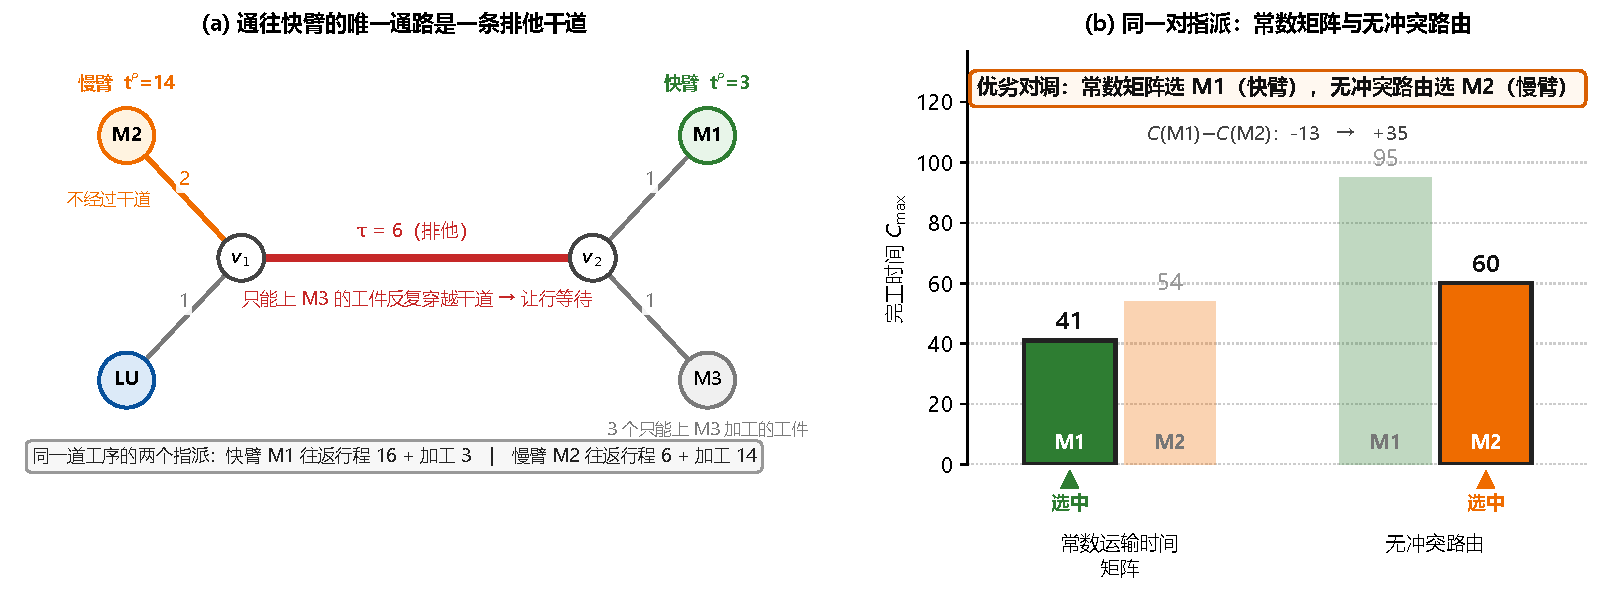
\includegraphics[width=\textwidth]{fig/fig_motivating_CN.pdf}
\Description{Two panels. The left panel is a small shop network in which the only
route to a fast arm passes through an exclusive trunk corridor, while a slow arm
hangs on its own branch. The right panel shows makespan for the same two machine
assignments evaluated twice: under a constant travel-time matrix the fast arm
wins, under conflict-free routing the slow arm wins, so the ranking reverses.}
\caption{动机算例:同一个指派决策,两种评价方式给出相反的次序。(a) 通往快臂 M1 的唯一通路是
一条排他干道($\tau=6$),慢臂 M2 接在一条不经过干道的短走廊上;另有三个只能上 M3 加工的工件运输需要反复穿越干道。
(b) 同一道工序的快臂、慢臂指派，分别用常数矩阵与无冲突路由评价。常数运输时间矩阵不含让行等待时间,故按"较短加工时间 $+$ 较长行驶时间"
选中快臂;把同样的指派交给无冲突路由重新评价,慢臂反而更优。差值由 $-13$ 翻为 $+35$。
本图是一个\emph{存在性演示}而非统计结论——它要说明反转会发生,不是反转肯定发生;在围绕该
算例的 $1200$ 组参数中有 $205$ 组($17\%$)出现反转,故它也不是参数空间里的孤点。}
\label{fig:motivating}
%% 由 fig/fig_motivating_CN.py 从 clbs/output/motivating.json 生成,后者由
%% clbs/tools/motivating.py --sweep 用与论文同一套解码器算出((b) 的四个数不是示意值:
%% 理想矩阵 = decode(conflict_free=False),无冲突路由 = decode(conflict_free=True))。
%% 算例:4 工件 / 3 机械臂 / 6 节点 / 5 走廊 / 2 AGV,delta_return=1,规则派车。
%% 注意:不要复用 fig/fig_intro_problem_new.pdf,那张图画的是上一篇论文
%% "邻近性对可用性"的场景,不是走廊争用。
\end{figure*}

\subsection{与已有工作的差距}

现有工作往往只处理柔性作业车间的排产，或只处理车辆的无冲突行驶；把两者融合在一起时，又通常先固定指派，再用路由消化争用，延误不能回头修改排产。
把柔性指派与无冲突路由写进同一个问题，已有精确方法在小规模上求至可证最优~\cite{vanos2026exact}；本文沿用这一已有问题设定，贡献在求解方法，不在问题定义。
算例规模一旦超出该精确分解所能证明最优的范围，现有文献方法仍把排产与无冲突路由分成先后两步：第一阶段先定机器指派与工序顺序，第二阶段再为这份已冻结的排产消解车辆冲突~\cite{sun2023integrated}。
第二阶段看到的走廊争用，不能回头修改第一阶段已经选定的机器与顺序。
即便加上反馈，也只是把一次执行得到的运输时长写回时间轴、且只作用于当前这一个解，既不修改机器指派，也不对搜索中的每个候选解重复这一步骤；其实验基准还是每道工序仅一台机器，不存在改派~\cite{li2026framework}。
因此，机器柔性、加工效率异构与走廊争用同时在场、且排产优化的是计入让行等待后的完工时间——这一权衡在已有文献里没有研究和表述。文献定位见第~\ref{sec:Chapter_II}~节。

\subsection{本文方法}

针对争用不能回头修改排产、搜索也不计入让行等待的缺口，本文用两条通路把排产与无冲突路由连起来，并分别度量每条通路对完工时间的贡献。框架使用双层结构——上层决定
机器指派与工序排序,下层以时间窗预约生成无冲突路径——但用评价与决策两条通路连接两层，并分别报告每条通路带来的完工时间变化。

\emph{评价通路}将每个候选解的适应度取为下层完成无冲突路由后的完工时间，让行等待因此进入搜索所优化的目标，而不再是事后做可行性校验。
一次无冲突解码的计算开销比按理想最短路矩阵解码高出约一个数量级；在固定算力下，更高的单次评价成本会减少可完成的评价次数。
\cite{li2026framework} 将「扩展为完全迭代的回路」列为未来工作，但未报告这一做法的计算代价及其对完工时间的影响。本文在同等挂钟预算下度量该权衡。

\emph{决策通路}采用\emph{预约表感知的车辆派遣}。一次运输分为空载取货与满载送货两段。
对每辆候选车，下层路由器在当前预约表上依次试算两段的最早可行时刻（试算过程中不写入最终时间表），
选中可行送达最早的车辆，而不是按理想最短路估计到达最早的车辆。该规则替换~\cite{li2026framework}
所用的空闲优先派车。为使单次评价在同等挂钟预算下保持\emph{低开销}，本文给出两项可证不改变输出的优化：
可采纳下界剪枝，以及胜者路径复用。

另外实现了两种层间接口：其一，对已被占用的走廊时段附加额外代价，使后续路径避开这些时段；其二，根据一次让行发生的走廊以及先行占用该走廊的运输，更换加工机器或调整工序顺序。
同等挂钟预算下，二者均未得到稳定的完工时间收益。报告它们是为了说明：在评价通路与决策通路之外继续加厚层间接口，并不是未尝试，而是在同等预算下没有转化为完工时间收益；
结果见第~\ref{sec:Chapter_V}~节。

\subsection{主要结果}

为分别度量闭环评价与预约表感知派遣各自的贡献，我们构造了一个四级基线阶梯,其中前两级分别复现两篇
已发表工作的结构:\textbf{B0} 为开环规划加真实执行,对应~\cite{li2026framework};\textbf{B0+}
在冻结排产上只把车辆指派换成感知冲突的,对应~\cite{sun2023integrated} 的两阶段结构;
\textbf{B1} 为闭环规划加规则派车;\textbf{B2} 为本文方法。这四级按两个维度排列：搜索时是否计入冲突造成的延误，以及按畅通时间选车还是按预约表试算选车。
因此，只有一次只改其中一个维度的对比，才能把收益记到对应机制上。
开环自报的完工时间在真实走廊上往往不可行。因此所有的排产方案都经同一套无冲突路由器执行，比较的一律是执行后可实现的完工时间。


结果显示两个维度上的对比都给出显著收益。把拥堵搬进搜索目标(固定派车方式)使完工时间降低
\GainLoopRule{}($p\PLoopRule$),这是闭环本身的价值;在闭环内部把规则派车替换为预约表
感知派遣(两者同为闭环，仅选车规则不同)再降低 \GainProbeLoop{}($p\PProbeLoop$),
这是该具体机制的价值;端到端相对文献结构降低 \GainEndToEnd{},\WinEndToEnd{} 胜
\LoseEndToEnd{} 负($p\PEndToEnd$)。两项降本使派遣机制的加速比达到 \SpeedupProbe{} 倍、
路由调用减少 \RouteCallCut{},单次评价的成本倍数从 \CostMultBefore{} 压到
\CostMultAfter{},这正是它在同挂钟预算下能够转为净收益的原因。

两条机制都显著,但\emph{不可互相替代}。开环下的预约表感知派遣值 \GainProbeOpen{}
($p\PProbeOpen$),远小于闭环的 \GainLoopRule{};端到端 \GainEndToEnd{} 接近两者独立时
应有的 \GainIndepProduct{},呈近加性,未检出正交互。
因此按两个维度分别报告，而不是只给一条从开环到完整方法的对照——后者会把大小悬殊的两笔收益混成一笔（派遣那几个百分点的收益会被闭环盖住），分开报告才能看出虽然派遣带来的收益小但仍显著。


按布局、车臂比与柔性分别报告的结果见第~\ref{sec:whichcongestion}~节。两条通路在各组算例上的表现不同。
对每组分别做显著性检验时，按上述三个方向做 Holm 校正：若不校正，\NCases{} 组里至少出现一处「显著」的概率会远高于名义水平。
校正后，闭环增益在 \CellsSigLoopAdj{}/\NCases{} 组上仍显著，并随争用强度大体上升，因而可以按布局方向解读。预约表感知派遣则无一组建组显著（校正前为 \CellsSigProbe{} 组）；
车臂比的四个水平上增益时正时负，且都到不了显著。
派遣只在把各组合计时显著；以每组 \NSeeds{} 个种子，尚不足以指出它在哪一类算例上稳定为正。

上述数字还依赖两条比较规则，细节见第~\ref{sec:protocol}~节。其一，各方法单次评价的计算开销可相差约两个数量级；若按相同搜索代数比较，等于让单次评价开销更高的方法多占用算力。
本文对齐的是同一段挂钟时间。其二，每次对比只改一个维度——搜索是否计入延误，或如何选车；若一次对比同时改了这两处，得到的只是合计，分不清收益来自闭环还是来自派遣。

\subsection{贡献}

\begin{enumerate}[leftmargin=*]

\item \textbf{问题层：柔性、效率异构与走廊争用同时在场时的改派权衡。} 机器柔性、加工效率异构与走廊争用同时在场，且排产优化的是计入让行等待后的完工时间时，通往快速机械臂的走廊拥堵，
一台较慢但连通性更好的机械臂可能是更优指派。用常数运输时间矩阵排产的模型看不见这一比较——矩阵不含让行等待~\cite{sun2023integrated}；
有无冲突路由、但每道工序机器固定的模型也没有这一比较，因为不存在改派~\cite{li2026framework}。
本文沿用已有的带无冲突运输约束的柔性作业车间调度设定~\cite{vanos2026exact}，贡献在求解方法，不在问题定义；
并补充一个可控的争用强度刻画，用以考察争用高到何种程度，把让行等待计入排产才带来收益。

\item \textbf{框架层：闭环双层框架，并度量路由内嵌评价对完工时间的贡献。} \emph{路由内嵌评价}将每个候选解的适应度取为下层完成无冲突路由后的完工时间，让行等待因此进入搜索所优化的目标。
一次无冲突解码的计算开销比按理想最短路矩阵解码高出约一个数量级；在固定算力下，更高的单次评价成本会减少可完成的评价次数。\cite{li2026framework} 将「扩展为完全迭代的回路」列为未来工作，
但未报告这一做法的计算代价及其对完工时间的影响。本文在同等挂钟预算下度量该权衡：相对开环（搜索时不计冲突），闭环使完工时间降低 \GainLoopRule（$p\PLoopRule$）；
在预约表感知派遣下，闭环相对开环降低 \GainLoopProbe（$p\PLoopProbe$）。

\item \textbf{机制层:预约表感知的车辆派遣,以及使它\emph{低开销}的两项优化。} 在闭环内部，把按畅通时间选车换成预约表感知派遣，完工时间再降低 \GainProbeLoop（$p\PProbeLoop$）。
该规则替换~\cite{li2026framework} 所用的空闲优先派车。本文给出两项优化——可采纳下界剪枝与胜者路径复用——并证明它们不改变所选车辆与最终时间表；
路由调用减少 \RouteCallCut，单次评价的成本倍数从 \CostMultBefore 降到 \CostMultAfter，加速比为 \SpeedupProbe。
车辆能力相同，差别只在当前位置与路段占用，因此预约表上的争用能够直接决定选哪辆车；改派机械臂则同时改变加工时间，工时差距常常大于走廊等待的差距。

\item \textbf{闭环与派遣的贡献大小不同，且派遣还不能指出在哪一类算例上稳定出现。} 闭环在 \CellsSigLoopAdj{}/\NCases{} 组上校正后仍显著；
预约表感知派遣的增益小得多，只在把各组合计时显著，端到端接近两因子独立复合时的预测值。
开环下只改选车，远不能代替把让行等待计入搜索。派遣在校正后无一组建组显著（校正前为 \CellsSigProbe{}/\NCases{} 组），车臂比的四个水平上增益时正时负。
合计显著只说明机制方向为正；以每组 \NSeeds{} 个种子，尚不足以指出它在哪一类算例上稳定兑现。
两条通路由四级基线阶梯分开度量。两种层间接口——对已占用走廊时段附加额外代价，以及按让行记录改派或调整顺序——作为对照写入第~\ref{sec:Chapter_V}~节，同等挂钟下均未得到稳定收益。


\end{enumerate}

全文符号汇总于表~\ref{tab:notation}。



\section{相关工作}
\label{sec:Chapter_II}

相关工作分两支。一支是带运输时间的柔性作业车间调度：决定什么在何处、以何种次序加工，车辆只作为能力资源，行驶时间取自常数矩阵。
另一支是无冲突多机器人路由：在时空上消解车辆争用，但不改任务的起点、终点与释放时刻。下面依次回顾这两支，再回顾把两者放进同一问题的工作，并最后落到本文所补的缺口说明。


\subsection{考虑运输的柔性作业车间调度}

含加工机器与运输车辆的柔性作业车间调度问题(FJSP\_PT)通过把物料移动纳入排程来扩展 FJSP。
Xin 等~\cite{xin2025review} 系统综述了该领域至 2023 年的进展,梳理其假设、约束、目标与
基准算例,并把求解方法分为精确、启发式、元启发式与群智能几类。一般柔性作业车间调度的建模、
约束与求解方法见同期综述~\cite{dauzereperes2024fjsp}。该族公开基准由 Homayouni 与 Fontes 整理~\cite{homayouni2021production}。
其中占主导地位的建模约定
是一个按位置对索引的常数行驶时间矩阵:车辆把工件从 $a$ 移到 $b$ 需要固定的 $t(a,b)$,
不随其他车辆是否占用同一走廊而改变。因此车辆只作为能力资源进入模型：有限车队为运输任务而竞争，进入走廊时段则不考虑约束。
% [ref_check: key=xin2025review; claim="该综述覆盖至 2023 年的进展,并将求解方法分为精确/启发式/元启发式/群智能四类"; need=quote]
% [ref_check: key=xin2025review; claim="常数行驶时间矩阵是 FJSP_PT 文献中占主导地位的建模约定"; need=quote]

在这一建模约定下，求解方法进展很快。Meng 等~\cite{meng2025cp} 给出多 AGV 情形下 FJSP 的约束
规划模型,关闭了 29 个此前开放的基准算例并改进了 27 个最优已知解,并与一个由约束规划辅助
的双种群遗传算法相配合。Qin 等~\cite{qin2026knowledge} 把质量--多样性存档与 Q 学习的区域
选择结合,并设计了由 AGV 与关键路径共同制导的局部搜索——但其关键路径仍是在矩阵行驶时间
上算出的。Fu 等~\cite{fu2025integrated} 用改进遗传算法在柔性装配车间中一体化地决策生产与
物流;其"一体化"指两类决策被同时求解,而非运输时长随排程而变。但在上述全部工作中,运输
时长都是从矩阵中读出的,因此一辆车永远不会被另一辆车因走廊争用而延误。
% [ref_check: key=meng2025cp; claim="关闭 29 个此前开放的基准算例并改进 27 个最优已知解"; need=quote]
% [ref_check: key=meng2025cp,qin2026knowledge,fu2025integrated; claim="三者的运输时长均取自常数矩阵,车辆之间不产生相互延误"; need=quote]

但是，这些假设"会降低问题复杂度,甚至改变问题的性质"~\cite{xin2025review};例如当运输车辆数量足够多时，工件到达机器的时刻在实践中受交通拥堵影响；
加工与运输两阶段之间的依赖必须先处理，排出的计划在真实走廊上才谈得上可行。
% [ref_check: key=xin2025review; claim="该综述把常数行驶时间矩阵本身列为局限性建模选择而非已成定论"; need=quote]
% [ref_check: key=xin2025review; claim="综述指出到达机器的时刻受交通拥堵影响,且加工-运输两阶段的隐含依赖须先处理"; need=quote]

这一支文献有机器柔性，却在常数运输时间矩阵上排产，因而可以把机器指派与工序排序推得很远。矩阵不含让行等待：
两条运输不会因争用互相推迟，指派的优劣也不随走廊占用而改变。
本文保留其柔性建模与元启发式求解框架，只把运输时长从矩阵中的常数换成无冲突路由后的通行时间——其中可以包含其他车辆造成的让行等待。

\subsection{任务外生的无冲突路由与拥堵感知派车}

另一支文献把走廊争用本身作为对象。多智能体路径规划（MAPF）要求若干智能体在共享图上无碰撞地从起点走到终点，其最优求解为 NP 难~\cite{gao2023mapf}；
单车在已被占用的图上寻路时，近年工作把安全区间规划接到二维路网与连续时间上~\cite{kasaura2022sipp}。
尤其是任务持续到达的设定下，拥堵在网络远未饱和时就会降低单位时间完成的任务数。
Zhang 等~\cite{zhang2024guidance} 优化一张带边权的路网，用边权把智能体从瓶颈处引开、减少迎面相遇，从而使若干持续到达任务的求解器完成更多任务。
在制造场景中，Kim 与 Kim~\cite{kim2026congestion} 为大规模 AGV 车队给出拥堵函数、拥堵惩罚与拥堵感知的派车规则，并在离散事件仿真中评估。
多 AGV 管理综述把派遣列为独立于路径规划的一层，空闲优先与最近车辆是其中常用的单属性规则~\cite{lu2022agv}；
自主移动机器人的规划与控制综述则把任务分配与路径规划列为同一控制栈上的相邻层~\cite{fragapane2021planning}。
% [ref_check: key=zhang2024guidance; claim="在终身式 MAPF 中拥堵于远未达到容量上限时即已损害吞吐"; need=quote]
% [ref_check: key=zhang2024guidance; claim="制导图抑制迎面运动并提升多个终身式求解器的吞吐"; need=quote]

这支文献有两点与本文直接相关。第一，任务的释放时刻、起点与终点是路由器的输入，路由器不能改产生这些任务的机器指派。
第二，对拥堵的量化通常不取某次运输实际发生的让行等待，而用间接指标：\cite{kim2026congestion} 看局部车辆密度，\cite{zhang2024guidance} 用离线学得的路网边权（权重越大，越不鼓励车辆走这条边）。
密度或边权只能表明某条走廊车辆偏多；一次让行则能指明哪条走廊、哪段时间、由哪次运输先占用。
% [ref_check: key=zhang2024guidance,kim2026congestion; claim="两者的任务释放时刻与起终点均为外生输入,路由器不参与任务生成"; need=quote]
% [ref_check: key=kim2026congestion; claim="其拥堵度量为局部车辆密度"; need=quote]
% [ref_check: key=zhang2024guidance; claim="其制导图边权为离线学得而非在线更新"; need=quote]

这一支具备真正的无冲突路由,却没有柔性可言:任务从别处来,指派不在它的决策范围之内。
本文保留其无冲突路径生成，让上层排产根据路由中发生的让行来改指派与工序顺序。

\subsection{调度与无冲突路由的一体化:反馈深度与本文定位}

把柔性指派与无冲突路由写进同一个问题的工作较少。van Os 与 Basten~\cite{vanos2026exact} 形式化了带无冲突运输约束的柔性作业车间调度：工序可选机器且加工时间随地点而变，车辆必须无冲突行驶。
求解用基于逻辑的 Benders 分解——约束规划主问题给出机器指派与工序顺序，整数规划子问题为该排程规划无冲突路径；
若路径不可行，子问题把冲突写成一条新约束送回主问题，禁止再出现同类排程。多数基准算例求至可证最优，其中约一半相对此前的启发式把完工时间改进了至少 10\%。
该方法受限于精确分解所能证明最优的算例规模。作者指出，更充分地利用「不可行是由哪些冲突造成的」这一信息，是自然的后续方向。
本文沿用这一已有问题设定，贡献在求解方法：在精确分解够不到的规模上，用启发式把路由中的延误送回排产决策。
% [ref_check: key=vanos2026exact; claim="多数基准算例求至可证最优,约半数相对既有启发式改进完工时间不少于 10%"; need=quote]
% [ref_check: key=vanos2026exact; claim="该方法的适用规模受限于精确分解可及的算例规模"; need=quote]

算例规模超出该精确分解之后，现有启发式仍把排产与无冲突路由分成先后两步。
Sun 等~\cite{sun2023integrated} 先用混合遗传算法定机器指派与工序顺序，再用带 AGV 编码的遗传算法与时间窗 Dijkstra 消解冲突；
第二阶段看到的争用，不能回头改第一阶段已经选定的机器与顺序。
Li 等~\cite{li2026framework} 加上一次反馈：路径层把实现的运输时长写回时间轴，只平移开工时刻，不改机器指派，且只作用于当前这一个解；
其基准还是每道工序仅一台机器，不存在改派。
% [ref_check: key=sun2023integrated; claim="第二阶段的冲突消解不反馈修改第一阶段的排程与指派"; need=quote]
% [ref_check: key=li2026framework; claim="其反馈内容仅为时间,且实验基准为每工序单一可选机器"; need=quote]

现有工作留下的缺口，不在于有没有处理车辆冲突，而在于路由结果如何进入排产。
Sun ~\cite{sun2023integrated} 与 Li ~\cite{li2026framework} 都已把无冲突行驶纳入流程；差别在于反馈的次数与内容——是每个候选解都用真实路由评价，还是只对当前这一个解做一次；
是只写回运输时长，还是让排产能据此改机器指派。

关键链推理是作业车间局部搜索中的成熟手段~\cite{otala2021graph,tamssaouet2023neighborhood}，近期带运输时间的柔性作业车间工作也加以使用~\cite{qin2026knowledge}。
但关键链若在常数行驶时间矩阵上计算，一次开工推迟只能追溯到前驱偏慢或机器繁忙，不能追溯到某条走廊——矩阵不含走廊占用。
本文改用时间窗预约的无冲突路由后，同一次推迟可以落到具体路段、具体时段，以及先行占用该路段的那次运输。
% [ref_check: key=qin2026knowledge; claim="关键链推理是作业车间局部搜索的成熟手段"; need=quote]

对算例设计,\cite{xin2025review} 指出该领域的算例"主要在规模上有差别,缺少针对关键问题
参数取值的专门设计",并特别把平均运输时间与平均加工时间之比 $\bar{T}_t/\bar{T}_p$ 列为
极可能影响算法表现的量,呼吁扩充测试集。本文在此之上补充一个只有在路由被显式建模后才可见
的参数:一个算例的拥堵中有多少是与指派相关的。集中在上下料出口的拥堵会被所有工件在所有
指派下穿越,因而不奖励任何决策;而只服务于部分机器的走廊上的拥堵则可以被绕开。两个
$\bar{T}_t/\bar{T}_p$ 完全相同的算例,留给调度机制的可操作余地可能完全不同。本文据此生成
争用强度可控的算例(第~\ref{sec:Chapter_V}~节)。
% [ref_check: key=xin2025review; claim="该综述把平均运输时间与平均加工时间之比列为极可能影响算法表现的参数,并呼吁扩充测试集"; need=quote]

表~\ref{tab:related} 汇总了上述比较。问题设定沿用~\cite{vanos2026exact} 已形式化的带无冲突运输约束的柔性作业车间调度，贡献不在问题定义。
敞开的是精确分解够不到的规模：此处排产与路由的连接仍然或缺失、或只先排产后消冲突、或只对当前这一个解反馈一次。
本文在这一规模上给出双层框架：每个候选解都用无冲突路由后的完工时间评价，并用预约表感知派遣按试算选车；两项优化压低单次评价开销，且不改变所选车辆与时间表。
闭环评价是较大的一笔收益，派遣是较小但仍显著的一笔，两者分开度量。

\begin{table}[t]
  \caption{相关工作与本文的对照。"机器异构"指一道工序有多台可选机器且加工时间随机器而变;
"耦合频次"指路由结果进入排产的次数与方向;
最后一列是反馈给排产的内容。本文每个候选解都用无冲突路由后的完工时间评价，并用预约表感知派遣选车。
本文实现了实现时间、让行记录与走廊时段加价三类接口,并按各自的代价与收益逐一报告。}
\label{tab:related}
%% 手工维护表:无生成脚本;任一行改动须同步 §2.3 正文。与 tab/ 下由 gen_tables_ladder.py 生成的表区分。
\footnotesize
\begin{tabular}{@{}lclll l@{}}
\toprule
工作类别 & 文献 & 机器异构 & 车辆争用 & 耦合频次 & 反馈内容 \\
\midrule
FJSP\_PT 元启发式 & \cite{meng2025cp,qin2026knowledge,fu2025integrated}
  & 有 & 常数矩阵 & --- & --- \\
终身式 MAPF & \cite{gao2023mapf,zhang2024guidance}
  & --- & 无冲突 & 任务外生 & 边权 \\
拥堵感知派车 & \cite{kim2026congestion}
  & 无 & 密度代理量 & 单向 & 拥堵惩罚 \\
两阶段 FJSP + 路由 & \cite{sun2023integrated}
  & 有 & 无冲突 & 单向 & 无 \\
强化学习调度 + PBS & \cite{li2026framework}
  & 无 & 无冲突 & 一次性修正 & 到达时刻 \\
精确 LBBD & \cite{vanos2026exact}
  & 有 & 无冲突 & 主--子问题 & 冲突驱动割 \\
\textbf{本文} &
  & 有 & 无冲突 & 每个候选解 & 实现时间 + 预约表试算 \\
\bottomrule
\end{tabular}
\end{table}


\section{问题描述与数学模型}
\label{sec:Chapter_III}
\subsection{问题描述}

一个算例由 $n$ 个工件、$N_M$ 台机械臂与 $N_A$ 辆自动导引车构成,它们在一个以图表示的车间路网
中运行。工件 $j$ 具有固定的 $n_j$ 道工序链 $O_{j1}\to\cdots\to O_{jn_j}$;工序 $O_{ji}$
可在其可选集 $\Omega_{ji}\subseteq M$ 中的任一机械臂上加工,在机械臂 $m$ 上耗时
$t^P_{jim}$,该值取决于所选的机械臂。机械臂占据图中的固定节点,工件由车队在这些节点之间
搬运。求解一个算例意味着同时确定四组决策:

\begin{enumerate}[label=(\roman*),leftmargin=*,topsep=2pt,itemsep=1pt]
\item 把每道工序 $O_{ji}$ 指派给某台机械臂 $m\in\Omega_{ji}$;
\item 为每台机械臂上被指派的工序排序;
\item 把由此派生的运输任务指派给车辆,并为每辆车的任务排序;
\item 为每一次车辆移动在图上规划路径,要求在时间与空间上无冲突,允许等待。
\end{enumerate}

目标是最小化完工时间 $C_{\max}$。

\begin{table}[t]
\caption{符号说明。}
\label{tab:notation}
\small
\begin{tabular}{@{}ll@{}}
\toprule
符号 & 含义 \\
\midrule
$J=\{1,\dots,n\}$, $O_{ji}$ & 工件集合;工件 $j$ 的第 $i$ 道工序,$i\le n_j$ \\
$M=\{1,\dots,N_M\}$, $\Omega_{ji}\subseteq M$ & 机械臂集合;$O_{ji}$ 的可选机械臂集 \\
$t^P_{jim}$ & $O_{ji}$ 在机械臂 $m\in\Omega_{ji}$ 上的加工时间 \\
$K=\{1,\dots,N_A\}$ & 同构的单载量车辆 \\
$G=(V,E)$, $\tau_e$ & 车间图;走廊 $e\in E$ 的通行时间 \\
$v_0$, $\mathrm{loc}(m)$ & 上下料站;机械臂 $m$ 所在节点 \\
$t^{*}(a,b)$ & $G$ 中 $a$ 到 $b$ 的最短路时间,不计争用 \\
$\delta_{\mathrm{ret}}\in\{0,1\}$ & 完工工件是否返回 $v_0$(基准取 $1$) \\
$S_{ji}$, $C_{ji}$, $A_{ji}$ & $O_{ji}$ 的开工、完工与物料到达时刻 \\
$C_{\max}$ & 完工时间 \\
\bottomrule
\end{tabular}
\end{table}

\subsection{建模假设}
\label{sec:assumptions}

\begin{enumerate}[label=\textbf{A\arabic*.},leftmargin=*,topsep=2pt,itemsep=2pt]
\item \textbf{静态算例与完全信息。} 全部 $n$ 个工件在 $t=0$ 时刻均已位于 $v_0$,不设释放
时刻与交货期。加工数据、布局 $G$ 与车辆状态在规划时均为已知。

\item \textbf{工件。} 每个工件具有固定的前后约束链。加工与运输均不可抢占,工件不可拆分,
不同工件之间不存在外生的先后约束。

\item \textbf{机械臂:部分柔性且工时异构。} 每道工序 $O_{ji}$ 可在任一
$m\in\Omega_{ji}$ 上加工,多数工序满足 $|\Omega_{ji}|\ge 2$,完全柔性
$\Omega_{ji}=M$ 是其特例。加工时间随所选机械臂而变，且不要求各臂之间存在统一的快慢关系:当
$m\neq m'$ 时,$t^P_{jim}$ 与 $t^P_{jim'}$ 不必成比例。一台机械臂同时只加工
一道工序,在计划期内不发生故障,与顺序相关的准备时间被并入 $t^P_{jim}$。

\item \textbf{缓冲区与装卸。} 每台机械臂的输入、输出缓冲区以及 $v_0$ 处的存储容量充裕,
因而不发生阻塞。装载与卸载时间可忽略,且不占用机械臂。

\item \textbf{车辆。} $N_A$ 辆车同构、单载量,空载与满载均以恒定速度行驶,不建模加减速与
电量;全部车辆在 $t=0$ 时空载停于 $v_0$ 且立即可用。一个运输任务是一次单程移动——从 $v_0$
到第一台机械臂、在前后两台不同机械臂之间,或当 $\delta_{\mathrm{ret}}=1$ 时从最后一台机械臂
返回 $v_0$;任一车辆可执行任一任务,
因此同一工件的连续移动可以在不同车辆之间接力。卸载之后车辆不被强制返回 $v_0$,而是按其
自身的任务链重新占位,且其出发时刻可由路由层推迟。

\item \textbf{路网与无冲突性。} $G$ 强连通,各走廊的通行时间 $\tau_e$ 为已知常数。走廊是
\emph{排他}资源:$e$ 的两个方向共享同一份预约,因而任一时刻最多一辆车占用 $e$,这同时
排除了迎面冲突与同向超车。占用区间取半开形式 $[t,\,t+\tau_e)$,故第二辆车可以恰好在
$t+\tau_e$ 进入。节点上设有容量充裕的停靠位,它与通行资源相互独立;因此等待发生在停靠位
上,并且总是被允许的。

\item \textbf{不在建模范围内。} 机器与车辆故障、有限缓冲与阻塞、电池充电,以及工件的动态
到达~\cite{gui2023dynamic,xiong2024dynamic}，留待后续工作（第~\ref{sec:future_work}~节第 (5) 条）。
\end{enumerate}

其中 A1、A2、A4 与 A5 在 FJSP\_PT 文献中是标准假设~\cite{xin2025review}。真正塑造本文的
是 A3(部分柔性机械臂上与机器相关的加工时间)与 A6(把争用表述为显式的排他资源约束,而不是
一个常数行驶时间矩阵),以及由此导出的一个事实:运输时长是路由决策的输出,而不是固定的输入参数。
无死锁不列为假设。它由 A4 与 A6 在第~\ref{sec:router}\ref{prop:decodable} 证明任意指派与工序顺序均可解码为无冲突、无死锁的时间表，因此搜索中不必对不可行解做修复。

\subsection{决策变量与派生的运输任务}

令 $x_{jim}\in\{0,1\}$ 表示 $O_{ji}$ 被指派给机械臂 $m$,记 $\mathrm{m}(j,i)$ 为所选机械臂,
$d_{ji}=\mathrm{loc}(\mathrm{m}(j,i))$ 为该臂所在节点。当 $\delta_{\mathrm{ret}}=1$时,
为每个工件追加一道位于 $v_0$、加工时间为零的\emph{伪工序} $O_{j,n_j+1}$,表示完工后返回上下料点;
这样，返回与中间搬运用同一套任务记号，完工时间一律取各工件最后一道工序的完成时刻。

与车辆路径问题不同,运输任务并不是输入的一部分,而是由指派\emph{派生}出来的:
\begin{equation}
\label{eq:tasks}
\mathcal{T}(x)=\Bigl\{\,(j,i)\ :\ d_{j,i-1}\neq d_{ji}\,\Bigr\},
\qquad d_{j0}\equiv v_0 ,
\end{equation}
其中任务 $(j,i)$ 把工件 $j$ 从 $d_{j,i-1}$ 搬到 $d_{ji}$,并在
$r_{ji}=C_{j,i-1}$ 时刻就绪(约定 $C_{j0}=0$)。若前后两道工序被放在同一台机械臂上,则不
产生任何运输任务。因此,运输任务的\emph{数量}与\emph{端点}都是决策组 (i) 的后果:一个把工件
始终留在同一台机械臂上的指派只需搬运两次,而一个每道工序都换臂的指派则需搬运 $n_j+1$ 次。
任务到车辆的指派用 $y_{tk}\in\{0,1\}$ 表示,对每个 $t\in\mathcal{T}(x)$ 有
$\sum_{k\in K}y_{tk}=1$,分给同一辆车的任务排成一条先后次序。

在常数行驶时间矩阵模型中，指派同样决定搬多少次、从哪到哪，但每次搬运的时长是矩阵里的常数，走廊占用不进入模型。
本文中，同一次指派还决定这些搬运会在哪些走廊上彼此争用。

\subsection{时序关系与可行性条件}

记 $p_{ji}=\sum_{m\in\Omega_{ji}}x_{jim}t^P_{jim}$ 为所选机械臂上的加工时间。对于指派、前后约束与
机械臂的单件加工能力给出
\begin{align}
\sum_{m\in\Omega_{ji}} x_{jim} &= 1, & \forall j,i,
\label{eq:assign}\\
C_{ji} &= S_{ji}+p_{ji}, & \forall j,i,
\label{eq:dur}\\
S_{ji} &\ \ge\ A_{ji}, & \forall j,i,
\label{eq:material}\\
S_{j'i'}\ \ge\ C_{ji}\ \ \vee\ \ S_{ji} &\ \ge\ C_{j'i'}
& \forall (j,i)\neq(j',i')\ \text{位于同一机械臂},
\label{eq:disj}
\end{align}
其中 $A_{ji}$ 是工件实际出现在 $d_{ji}$ 的时刻。若 $(j,i)\notin\mathcal{T}(x)$,则工件
本已在该处,$A_{ji}=C_{j,i-1}$。否则 $A_{ji}$ 由承运任务 $(j,i)$ 的那辆车产生:记
$a^{\mathrm{E}}_{ji}$ 为该车经空载段到达取货节点的时刻,则
\begin{equation}
\label{eq:load}
\ell_{ji}=\max\bigl(a^{\mathrm{E}}_{ji},\ r_{ji}\bigr),
\qquad
A_{ji}=\text{于 } \ell_{ji} \text{ 出发的满载段的到达时刻},
\end{equation}
即车辆可以等工件,工件也可以等车辆。无论空载段还是满载段,每一段都是 $G$ 中的一条通路
$(e_1,\dots,e_q)$,其走廊进入时刻 $\eta_1,\dots,\eta_q$ 满足
\begin{equation}
\label{eq:walk}
\eta_1 \ \ge\ \sigma, \qquad
\eta_{l+1}\ \ge\ \eta_l+\tau_{e_l}, \quad l=1,\dots,q-1,
\end{equation}
其中 $\sigma$ 是该段可以开始的时刻;
进入下一走廊的时刻若正好等于本段走完的时刻，则中间不停；若进入下一走廊的时刻晚于本段走完的时刻，中间差额即车辆在停靠位等待。该段在 $\eta_q+\tau_{e_q}$ 结束。
最后是走廊争用约束:
\begin{equation}
\label{eq:excl}
\bigl[\eta,\ \eta+\tau_e\bigr)\ \cap\
\bigl[\eta',\ \eta'+\tau_e\bigr)\ =\ \emptyset
\end{equation}
该式对同一走廊 $e$ 的任意两次不同占用都成立,与方向无关,也与涉及哪些车辆无关。目标函数为
\begin{equation}
\label{eq:obj}
\min\ C_{\max},\qquad
C_{\max}=\max_{j\in J}\ C_{j,\,n_j+\delta_{\mathrm{ret}}} .
\end{equation}

有两个推论值得记录,因为第~\ref{sec:Chapter_IV}~节的算法正建立在它们之上。第一,在任何
半活动排程中,\eqref{eq:material} 与 \eqref{eq:disj} 可收紧为
\begin{equation}
\label{eq:bind}
S_{ji}=\max\bigl(A_{ji},\ F_{\mathrm{m}(j,i)}\bigr),
\end{equation}
其中 $F_m$ 是机械臂 $m$ 上排在 $O_{ji}$ 之前那道工序的完工时刻。因此开工时刻等于工件到达时刻与该臂上一道工序完工时刻二者中的较晚者；哪一个更晚，比较即可得出。
后文据此把一次开工推迟追溯到待料或待臂。第二,\eqref{eq:excl} 是模型中唯一通过\emph{空间}而非通过共享机器来耦合不同工件的约束。

\subsection{与 FJSP\_PT 的关系}
\label{sec:fjsppt}

去掉~\eqref{eq:excl} 后，各段行驶不再互相占用走廊，于是每一段都可以走最短路，且中间不必等待。运输时长退化为常数矩阵 $t^{*}(a,b)$,
模型即成为带运输时间的柔性作业车间调度（FJSP\_PT）。两个问题的差别因此只在这组走廊排他约束：有它，一次移动的时长由各车路径共同决定；没有它，时长是输入参数。
由此得到的 $t^{*}$后文用作下界，也在开环基线中用来按畅通行驶时间估计到达时刻。本文在 FJSP\_PT 上增加这组约束，沿用其问题设定。

与同样给出显式路网的工作相比，差别在于预约的对象。van Os 与 Basten~\cite{vanos2026exact}
预约的是\emph{节点}：两车不得同时占据同一节点，也不得交换节点。本文预约的是\emph{边}：走廊双向排他，任一时刻至多一辆车占用一条走廊。
Lyu 等~\cite{lyu2019approach} 同样是双向路网、边排他，但还要求任一节点同时只容一辆车；本文不设这一节点容量约束，等待发生在充裕的停靠位上。
算例不能直接对比的原因见第~\ref{sec:limitations}~节局限 (1)。

\subsection{计算复杂度}

\begin{prop}
\label{prop:np_hard}
由 \eqref{eq:assign}--\eqref{eq:obj} 定义的问题是强 NP 难的;且当所有工序均满足
$\Omega_{ji}=M$ 时依然如此。
\end{prop}

\begin{proof}
限制到如下算例:对所有 $e\in E$ 有 $\tau_e=0$,每台机械臂各由一条专用走廊与 $v_0$ 相连,
且 $N_A=n$。此时每一段行驶耗时为零、占用的半开区间 $[t,t)=\emptyset$,故 \eqref{eq:excl}
恒真,任何车辆都无法延误另一辆车;又因每个工件独占一辆车,\eqref{eq:load} 从不起作用,
$A_{ji}=C_{j,i-1}$。余下的正是取 $A_{ji}=C_{j,i-1}$ 的
\eqref{eq:assign}--\eqref{eq:disj},也就是无关机器情形下的柔性作业车间调度问题。它的两个
特例已是强 NP 难的:处处取 $|\Omega_{ji}|=1$ 时退化为经典作业车间问题,在三台机器下即为
强 NP 难;取 $\Omega_{ji}=M$ 且 $n_j=1$ 时退化为无关并行机上
的完工时间最小化问题,它包含同型并行机调度,在机器数可变时为强 NP 难。
一般柔性作业车间调度本身即为强 NP 难~\cite{dauzereperes2024fjsp}。上述每个限制均为
多项式规约,故一般问题是强 NP 难的;第二个特例同时说明完全柔性并不会使问题变容易。
\end{proof}

命题~\ref{prop:np_hard} 的规约把走廊通行时间设为零，从而排除车辆争用。这说明即使没有走廊争用，问题已是强 NP 难。
再把决策 (i)--(iii) 固定之后，剩下的路径规划仍是一个无冲突多智能体路由问题~\cite{gao2023mapf}，且各任务的释放时刻与端点由工序链和指派决定、彼此牵制。
因此无冲突路由是在调度难度之上增加约束，而不是替换它。小规模上已有精确方法：van Os 与 Basten~\cite{vanos2026exact} 用基于逻辑的 Benders 分解，
将同一问题设定下的多数基准算例求至可证最优。本文处理的是该精确分解够不到的规模。

\subsection{算例特征的刻画}
\label{sec:features}

本文固定算例规模，只改变其结构；规模本身的影响见第~\ref{sec:limitations}~节局限 (1)。
每个算例记录下列特征。前四项是调度文献中的常用量；Xin 等~\cite{xin2025review} 指出，其中 $\bar{T}_t/\bar{T}_p$ 很可能影响算法表现。


\begin{itemize}[leftmargin=*,topsep=2pt,itemsep=1pt]
  \item $\bar{T}_t/\bar{T}_p$：机械臂节点之间的平均最短路行驶时间除以平均加工时间，即运输时间相对加工时间的比值。
  \item 异构度 $H$：各工序在可选机械臂上加工时间的变异系数，再对所有工序取平均（$|\Omega_{ji}|=1$ 的工序按 $0$ 计入）。
  $H=0$ 表示可选臂工时相同，改派不再有加工时间上的得失，但仍可换臂以避开拥堵，且此时换臂不增加工时。
  第~\ref{sec:whichcongestion}~节按 $H$ 分组的实测与此相符，故不以 $H$ 的增大预期更大收益。
  \item 柔性度 $F=\operatorname{mean}_{ji}|\Omega_{ji}|/N_M$：每道工序平均可选机械臂数占全部机械臂的比例，即可改派的范围。
  \item $N_A/N_M$：车辆数与机械臂数之比。比值偏小则瓶颈更可能在运输，偏大则更可能在加工。
\end{itemize}

上列四项之外，再记两个只在显式路网上才有意义的量。要看的不是拥堵有多严重，而是其中有多少可以通过改派避开。
令 $\mathrm{cut}(v_0)$ 为切断上下料点 $v_0$ 与所有机械臂之间通路所需删去的最少走廊集合。

\begin{itemize}[leftmargin=*,topsep=2pt,itemsep=1pt]
  \item 争用强度：在初始随机种群上，让行等待占行驶总时间的比例。它由算例结构读出，不是输入参数，本文用它给算例排序，各组数值见表~\ref{tab:instances}。
  \item $|\mathrm{cut}(v_0)|$（漏斗宽度）：可同时离开上下料点的车辆数上界。取 $1$ 表示所有车辆必须经过同一条走廊才能离站。布局一组正是通过增加或减少这类并行出口来改变争用；\texttt{funnel} 相对 \texttt{high}，该值减半。
\end{itemize}

另记一个试过但未采用的量。
\emph{漏斗占比} $\varphi\in[0,1]$ 为一次典型的 $v_0\to$机械臂行程中，花在\emph{所有}最短 $v_0\to$机械臂路径都共用的走廊上的时间比例。
这类走廊在任何指派下都会被每个工件经过，其上的延误不随决策 (i)--(iii) 改变；$\varphi$ 越大，改派越难避开拥堵。
它本应用来区分可避开与避不开的拥堵，这是争用强度做不到的。
但在本文算例上，两个按构造应当不同的布局给出了几乎相同的 $\varphi$，故未进入后文分析，仅在此记录定义。
设计能区分这两类布局的指标列为后续工作（第~\ref{sec:future_work}~节第 (1) 条）。
另曾用远组割——隔离到 $v_0$ 距离超过中位数的那些机械臂所需删去的最少走廊数——刻画远离上下料点的瓶颈容量；
在本文的单一布局模板下它与 $|\mathrm{cut}(v_0)|$ 几乎相同，同样不进入分析。

每个算例附带一个由算例数据直接算出的复合下界
$\mathrm{LB}=\max(\mathrm{LB}_{\text{chain}},\mathrm{LB}_{\text{load}},
\mathrm{LB}_{\text{cut}})$。三个分量各自放松模型的不同部分，没有一个在所有算例上总是最大。
$\mathrm{LB}_{\text{chain}}$ 对每个工件取「最短入场行程 $+$
$\sum_i \min_{m\in\Omega_{ji}}t^P_{jim}$ $+$ 最短返回行程」，即不计臂间搬运与全部排队。
$\mathrm{LB}_{\text{load}}$ 取 $\sum_{j,i}\min_m t^P_{jim}/N_M$，即不计工序先后与运输。
$\mathrm{LB}_{\text{cut}}$ 利用漏斗：当 $\delta_{\mathrm{ret}}=1$ 时每个工件穿越
$\mathrm{cut}(v_0)$ 两次；把 $X=2n$ 次穿越分到该割集的各条走廊上，使最繁忙一条的负载最小，得到
\begin{equation}
\label{eq:lbcut}
C_{\max}\ \ge\ X\Bigl/\sum_{e\in \mathrm{cut}(v_0)}\tau_e^{-1}.
\end{equation}
在本文算例上，三者中取到最大的是 $\mathrm{LB}_{\text{cut}}$（十组中八组）与
$\mathrm{LB}_{\text{chain}}$（其余两组），$\mathrm{LB}_{\text{load}}$ 从未最大——这与争用集中在上下料出口的算例设计相符。
该下界是松的：与已知最好解的间隙大约在 \LBGapLo{} 到 \LBGapHi{} 之间，故只用于核对数量级，不用来证明解已接近最优。

\section{闭环双层框架}
\label{sec:Chapter_IV}
\subsection{框架总览:路由内嵌评价与决策通路}
\label{sec:overview}

本框架把第~\ref{sec:Chapter_III}~节的四组决策分配到两层。输入是一个算例:工件的工序链、
机器的可选集与工时、车队规模与走廊网络。上层用一个 memetic 算法在指派与排序上搜索~\cite{zhang2024memetic};中间由
一个事件驱动的解码器把上层的一个候选解翻译成一串带先后约束的运输任务;下层以时间窗预约把
这串任务转化为无冲突路径。输出是一张可执行的无冲突时间表及其完工时间。
与两阶段方案或只修正一次的方案相比，差别不在于分成两层，而在于路由结果如何进入排产：反馈什么、沿哪个方向，以及每个候选解是否都反馈一次。


\begin{description}[leftmargin=0pt,topsep=3pt,itemsep=3pt]
  \item[评价通路，即\emph{路由内嵌评价}。]
  每一代中每一个候选解的适应度，都取下层完成全部运输任务的无冲突路由之后的完工时间，其中已含让行等待。
  上层优化的就是这个数，而不是按理想最短路算出的完工时间。
  \item[决策通路。]
  选车时可以读取当前预约表，而不是等路径生成完毕再看结果。
  具体机制是\emph{预约表感知的车辆派遣}：对每辆候选车，在预约表上依次试算空载段与满载段的最早可行时刻（试算不写入最终时间表），选可行送达最早的车辆，而不是按畅通最短路估计到达最早的车辆。
\end{description}

评价通路让搜索优化计入让行等待后的完工时间；决策通路让选车依据预约表上的试算，而不是畅通时间估计。
两条通路对完工时间的贡献在第~\ref{sec:Chapter_V}~节分别度量：闭环评价是较大的一笔，预约表感知派遣是较小但仍显著的一笔，端到端接近两因子独立复合时的预测值。
开环下只改选车，远不能代替把让行等待计入搜索。

另外实现了两种层间接口：其一，对已被占用的走廊时段附加额外代价（后文称加价），使后续路径避开这些时段；其二，按让行记录改派或调整顺序。
同等挂钟预算下，二者均未得到稳定的完工时间收益。
构造见第~\ref{sec:interface}、\ref{sec:ls}~节，结果作为对照见第~\ref{sec:Chapter_V}~节。

框架结构见图~\ref{fig:framework}。两条通路进入上层的位置不同，因而单次评价的计算开销也不同。

%% 本图由 fig/fig_framework_CN.py 生成,是一张示意图,不含任何数据。
%% 注意不要复用 fig/fig_hdp_architecture*.pdf,那是上一篇论文的 HDP 框架。
\begin{figure*}[t]
\centering
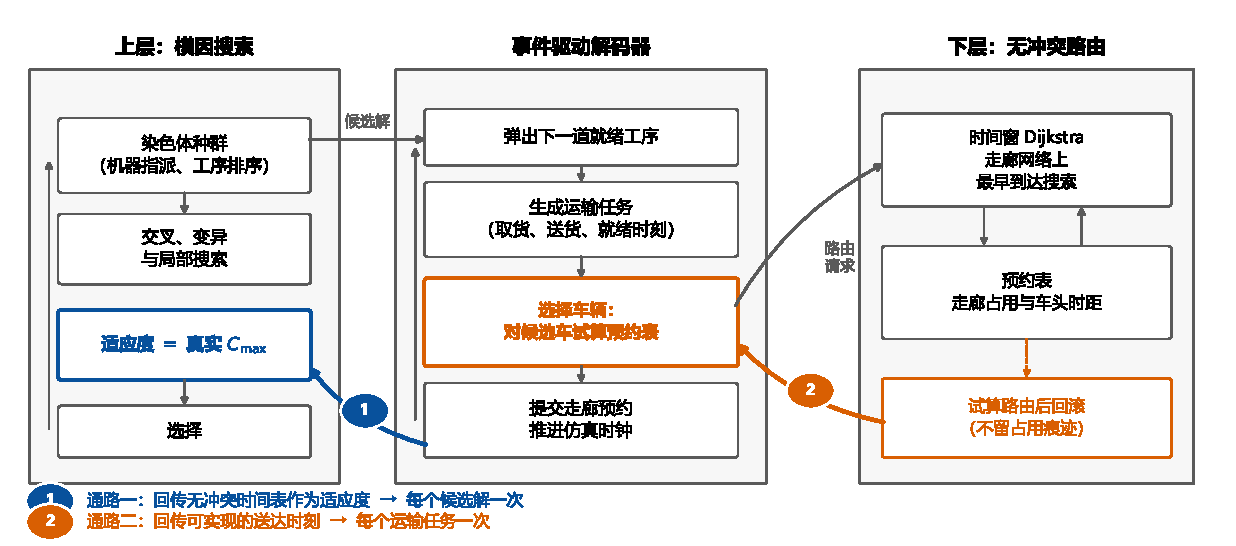
\includegraphics[width=\textwidth]{fig/fig_framework_CN.pdf}
\caption{闭环双层框架。上层以 memetic 算法搜索指派与排序，下层以时间窗预约做无冲突路由，
中间的事件驱动解码器把上层的一个候选解翻译成一串运输任务。
两条反馈通路以颜色区分，进入上层的位置不同：
通路一（蓝，标记 1）把下层完成的无冲突时间表作为适应度回传，每个候选解评价一次；
通路二（橙，标记 2）在选车前于预约表上试算两段的最早可行送达时刻，每个运输任务试算一次，试算不写入最终时间表。
第~\ref{sec:Chapter_V}~节的四级基线阶梯按这两条通路是否打开排列。}
\Description{Schematic of the closed-loop bilevel framework: an upper memetic
search layer, an event-driven decoder, and a lower time-window reservation
routing layer, with two colour-coded feedback paths entering the upper layer at
different places---the evaluation path returning a realized makespan once per
candidate, and the decision path returning a realizable arrival time once per
transport task.}
\label{fig:framework}
\end{figure*}

\subsection{下层:时间窗预约与无冲突路由}
\label{sec:router}

\subsubsection{预约表}
唯一被争用的资源是走廊（假设 A6），因此预约表把每条走廊映射到一个按时间排序的半开占用区间列表 $[t,\,t+\tau_e)$，每个区间标注占用它的车辆与任务。
该表支持四种操作：查询不早于某时刻的最早可行进入时刻；写入一次占用；撤销某任务的全部占用；以及保存当前表状态并在试算后恢复（检查点与回滚）。
节点不被预约：穿越节点耗时为零，等待发生在停靠位上（假设 A6 已把停靠位与通行资源分开）。
因此只需预约走廊这一种资源，下层路由器与独立于解码器的校验器都只检查走廊占用。

\subsubsection{时间窗 Dijkstra}
一段行驶用标签设定（label-setting）搜索来规划。标签 $(u,t)$ 表示「在时刻 $t$ 停在节点 $u$ 的停靠位上」，代价为 $t$（算法~\ref{alg:route}）。
考察一条从当前节点出发的走廊时，向预约表查询最早可行进入时刻 $t'\ge t$；间隔 $t'-t$ 即车辆在 $u$ 的停靠位上等待的时间。
\eqref{eq:walk} 中的等待因此由搜索直接给出，不必另行建模。
在一次解码内，已写入预约表的路径不再撤销，故车辆按解码器生成任务的固定次序依次规划，后规划的车避让先规划的车。

\begin{lem}[最早到达即充分]
\label{lem:label}
每个节点只保留到达最早的标签，即可得到在当前预约表下最早到达终点的路径。
\end{lem}

\begin{proof}
  停靠位容量充裕且不占用通行资源（A6），因此一辆自时刻 $t$ 起停在 $u$ 的车，只需继续等到 $t'$，
  就能走出任何在 $t'>t$ 才到达 $u$ 的车所能走的后续路径。
  故更早到达的标签不会更差，每个节点只需保留到达最早的那一个。
  又因向预约表查询的时刻越晚，尚且可行的进入时段只减不增，
  进入走廊 $e$ 并走完它的时刻
  $t\mapsto R.\textsc{EarliestEntry}(e,t,\tau_e)+\tau_e$
  关于 $t$ 单调不减。
  搜索按到达时刻从小到大取出标签，终点第一次被取出时即为最早到达。
\end{proof}

因此每个节点只需保留一个最早到达标签，用普通 Dijkstra 即可，不必采用安全区间规划（SIPP）那种按可行时段分标签的做法~\cite{kasaura2022sipp}。
若再引入第二项指标（例如占用繁忙走廊时段的额外代价），更早到达不再总是更好，每个节点必须保留多个互不占优的标签。
第~\ref{sec:interface}~节回到这一点：这也是走廊时段附加代价在同等挂钟预算下未能带来稳定完工时间收益的原因之一。

\begin{algorithm}[t]
  \caption{\textsc{Route}:无冲突的单段路径规划}
  \label{alg:route}
  \small
  \begin{algorithmic}[1]
  \Require 起点 $s$、终点 $g$、最早出发时刻 $t_0$、预约表 $R$、是否写入预约表的标志 \textit{commit}
  \Ensure 到达时刻与走廊占用区间的序列；若 \textit{commit} 为真，这些区间同时写入 $R$
  \State 将标签 $(s,t_0)$ 放入以（时间，节点标识）为键的优先队列
         \Comment{时刻相同时按节点标识决定先后，次序确定}
  \While{队列非空}
    \State 取出键最小的标签 $(u,t)$
    \If{$u=g$} \State 回溯得到各占用区间；若 \textit{commit} 为真则逐一写入 $R$；
         \Return 到达时刻 $t$ \EndIf
    \ForAll{自 $u$ 出发的走廊 $e=(u,v)$}
      \State $t_{\text{in}} \gets R.\textsc{EarliestEntry}(e,t,\tau_e)$
         \Comment{在 $u$ 的停靠位等到 $t_{\text{in}}$}
      \State 若 $t_{\text{in}}+\tau_e$ 严格早于 $v$ 的已有到达时刻，则更新标签 $(v,\ t_{\text{in}}+\tau_e)$
    \EndFor
  \EndWhile
  \State \Return 失败 \Comment{$G$ 强连通时不应发生，见正文}
  \end{algorithmic}
\end{algorithm}

预约次数有限、时间有界，且 $G$ 强连通，故路径总是存在：最坏情况下车辆一直等到已有占用全部结束，再按畅通最短路行驶。
这一点保证下文命题~\ref{prop:decodable} 成立，因此搜索中不必对不可行解做修复。
单次调用的代价为 $O\bigl(|E|\,(W^{2}+\log|V|)\bigr)$：至多考察 $|E|$ 条走廊，每条先枚举 $O(W)$ 个候选进入时刻，再对每个候选做一次 $O(W)$ 的重叠判定，
并做一次 $O(\log|V|)$ 的堆操作，其中 $W$ 为每条走廊上预约区间数的均值。
若预约表改为支持对数时间最早进入查询的有序结构，复杂度可降至 $O\bigl(|E|(\log W+\log|V|)\bigr)$；本文实现用的是上述线性扫描。

对空预约表，在所有取货--送货节点对上运行同一搜索，即得到第~\ref{sec:Chapter_III}~节的畅通最短路矩阵 $t^{*}$。
它用于三处：开环配置里按畅通时间估计到达时刻、改派邻域中的邻近项，以及两阶段基线的运输时间；同时也是第~\ref{sec:speedup}~节剪枝所用的可采纳下界。


\subsection{上层:编码与事件驱动解码}
\label{sec:upper}

\subsubsection{染色体编码}
设工序总数为 $N$。一个个体由两段构成：长度为 $N$ 的\emph{机器指派向量}，按固定枚举，第 $k$ 个分量是第 $k$ 道工序在 $\Omega_{ji}$ 中所选的机械臂；
以及\emph{工序序列}，即允许同一工件多次出现的排列——工件 $j$ 出现 $n_j$ 次，第 $x$ 次代表 $O_{jx}$。
该序列给出全局先后：共用同一台机械臂的工序，相对顺序由它读出。

当 $\delta_{\mathrm{ret}}=1$ 时，每个工件在序列中额外出现一次，对应第~\ref{sec:Chapter_III}~节的伪工序（地点固定为 $v_0$，加工时间为零）。
返回运输因此与中间运输使用同一套指派与排序，解码时不必另写分支。

任务派给哪辆车不写入染色体，而在解码时决定（第~\ref{sec:dispatch}~节）。
若另设第三段表示派车，搜索空间会扩大，且不能再保证任意染色体均可解码，从而需要修复算子。


\subsubsection{事件驱动解码器}
解码器(算法~\ref{alg:decode})就是评价通路。它自左向右扫过工序序列,为每台机械臂维护其空闲
时刻,为每个工件维护其当前节点与就绪时刻,为每辆车维护其当前节点与可用时刻。当某道工序的
机械臂与工件当前位置不同时,便生成 \eqref{eq:tasks} 的运输任务,选定一辆车,并针对\emph{实时
的}预约表规划两段路径:到取货点的空载段与到目的地的满载段,两者由 \eqref{eq:load} 衔接。
随后工序按 \eqref{eq:bind} 开工；解码器同时记下两项中哪一项更大，记为 \texttt{bind} 字段，后文追溯开工推迟时以它为准。

\begin{algorithm}[t]
\caption{\textsc{Decode}:以完整无冲突仿真作为适应度}
\label{alg:decode}
\small
\begin{algorithmic}[1]
\Require 算例、路网、指派 $x$、工序序列
\Ensure 完工时间、时间表、逐走廊的让行统计量
\State 对所有机械臂置 $F_m\gets 0$;对所有工件置 $\mathrm{pos}_j\gets v_0$,
       $\mathrm{ready}_j\gets 0$
\State 对所有车辆置 $\mathrm{loc}_k\gets v_0$、$\mathrm{avail}_k\gets 0$;清空预约表
\ForAll{按序列次序取出的工序 $O_{ji}$(含伪工序)}
  \State $m\gets$ 在 $x$ 下 $O_{ji}$ 的机械臂;$d\gets \mathrm{loc}(m)$
  \If{$\mathrm{pos}_j=d$}
     \State $A_{ji}\gets \mathrm{ready}_j$ \Comment{同臂连续,不生成运输任务}
  \Else
     \State 选定车辆 $k$(第~\ref{sec:dispatch}~小节)
     \State $a^{\mathrm{E}}\gets\textsc{Route}(\mathrm{loc}_k,\mathrm{pos}_j,
            \mathrm{avail}_k,R,\text{真})$;\ \ $\ell\gets\max(a^{\mathrm{E}},
            \mathrm{ready}_j)$ \Comment{空载段同样占用走廊}
     \State $A_{ji}\gets\textsc{Route}(\mathrm{pos}_j,d,\ell,R,\text{真})$;\ \
            $\mathrm{loc}_k\gets d$;\ \ $\mathrm{avail}_k\gets A_{ji}$
     \State 按走廊累计让行时间
  \EndIf
  \State 若 $F_m>A_{ji}$ 则 $\texttt{bind}\gets\texttt{machine}$,否则
         $\texttt{bind}\gets\texttt{arrive}$
  \State $S_{ji}\gets\max(A_{ji},F_m)$;\ \ $C_{ji}\gets S_{ji}+p_{ji}$;\ \
         $F_m\gets C_{ji}$;\ \ $\mathrm{pos}_j\gets d$;\ \
         $\mathrm{ready}_j\gets C_{ji}$
\EndFor
\State \Return $C_{\max}=\max_{j,i} C_{ji}$、时间表与逐走廊的让行统计量
\end{algorithmic}
\end{algorithm}

由此得到两条性质。其一，预约按解码器生成任务的次序写入；两处时刻相同时均按固定规则决定先后——路由的标签队列以（到达时刻，节点标识）为键，且仅当新到达严格更早时才更新标签；
派车按车辆编号升序扫描，保留首个严格更优者（第~\ref{sec:speedup}~节）。
因此一个染色体总对应唯一一张时间表，评价是确定性的。第~\ref{sec:Chapter_V}~节按种子配对、比较同一预算下的结果，依赖这一点。
其二，解码只向前推进：若邻居只改动序列位置 $x$ 之后的部分，则 $x$ 之前的事件与预约均保持不变。
这是增量评价的基础；当前实现尚未使用这一加速。

\begin{prop}[任何染色体都可解码]
  \label{prop:decodable}
  对任意机器指派与任意工序序列，算法~\ref{alg:decode} 均终止，并返回一张无冲突、无死锁且完工时间有限的时间表。因此搜索中不必调用修复算子。
\end{prop}

\begin{proof}
  按编码方式，工序序列是各工件前后约束的一个拓扑序：工件的第 $x$ 次出现代表其第 $x$ 道工序，因此读取 $\mathrm{ready}_j$ 时该值已知。
  缓冲区充裕（A4）意味着工序不会因无处存放而阻塞，故工件一经到达，\eqref{eq:bind} 总给出有限开工时刻。
  每次 \textsc{Route} 调用按算法~\ref{alg:route} 之后的论证在有限时间内返回，且只占用预约表上尚未占用的时段，故 \eqref{eq:excl} 由构造成立。
  无死锁同样由构造得到：走廊是唯一被争用的资源（A6），等待只发生在容量充裕的停靠位上、不占用走廊；已写入预约表的占用均在有限时刻结束，因此不存在互相等待的车队——最坏情况下，一辆车等到已有占用全部结束后即可通行。
  扫描共执行 $N+n\delta_{\mathrm{ret}}$ 次，每次在有限时刻上安排有限个事件。
\end{proof}

%% 原为 4.3 的一个子小节 "Dispatching",现提升为独立一节:它是本文承重的机制,
%% 不应埋在"上层编解码"之下。原 4.4 "What should cross the interface?" 的三种接口
%% 讨论降为本节的一个子小节,作为选定该机制的论证。
\subsection{预约表感知的车辆派遣}
\label{sec:dispatch}

选车既可以按畅通最短路时间估计，也可以按预约表上的试算。开环规则对每辆车打分
\begin{equation}
\label{eq:rule}
\mathrm{score}(k)=\max\bigl(\mathrm{avail}_k+t^{*}(\mathrm{loc}_k,\text{取货点}),\,
\mathrm{ready}_j\bigr)+t^{*}(\text{取货点},\text{目的地}),
\end{equation}
它不查预约表，因此可能选中几何上近、走廊上却已占用的车辆。
该式与~\cite{li2026framework} 的空闲优先派车相同，也是多 AGV 派遣综述中的典型单属性规则~\cite{lu2022agv}。

闭环默认改为\emph{预约表感知的车辆派遣}。对每辆候选车：先把空载段写入预约表并规划，再在不写入最终时间表的前提下规划满载段，记下试算得到的最早可行送达时刻，然后把预约表恢复到试算前。
空载段必须先写入，否则满载段看不见这段占用，两段可能被排进同一走廊的同一时段，试算会偏早。
选中的是可行送达最早的车辆，而不是 \eqref{eq:rule} 估计最优的车辆。

车辆能力相同（假设 A5），差别只在当前位置与路段占用，因此预约表上的争用能够直接决定选哪辆车。
改派机械臂则同时改变加工时间，工时差距常常大于走廊等待的差距，故同一套试算用在选臂上收益很小。

代价同样具体：试算把每个运输任务的路由调用从 $2$ 次增至至多 $2N_A$ 次，单次评价成本约为按畅通时间选车的 \CostMultBefore{} 倍。
若不压低这一开销，同等挂钟预算下机制带来的完工时间收益会被额外计算吃掉。
两项加速见第~\ref{sec:speedup}~节；第~\ref{sec:Chapter_V}~节因此只在同一挂钟时限下比较两种派车。

\subsubsection{层间接口的三种选择}
\label{sec:interface}

两层既已固定，接下来的选择是下层向排产回传什么。本文实现了以下三种，并在同等挂钟预算下分别度量。
预约表感知派遣属于第一种，也是其中唯一带来稳定完工时间收益的；另外两种的构造写在下面，结果见第~\ref{sec:Chapter_V}~节。

\paragraph{只回传实现时长。}
下层返回无冲突路由后的通行时间。这正是评价通路已经在做的事，也是预约表感知派遣在试算时读取的量。
它使每个候选解按计入让行等待后的完工时间排序，但不指出是哪一项决策导致了等待。
先排产再路由一次的方法连这一点也做不到：它们只在指派固定之后才得到一次真实时长。
本文的主要收益即来自这里：搜索比较的每一个候选解，其适应度都已包含该解自身引起的让行等待。

\paragraph{回传走廊时段的额外代价。}
与拉格朗日松弛及列生成中的协调相类比，下一步是给被争用的资源加价：为每个走廊--时段槽位附影子价格 $\pi(e,b)$，
让路径规划在 Pareto 前沿上最小化「到达时刻 $+\theta\cdot$代价」（$\theta\ge0$ 为唯一旋钮），并让改派为所需通行付出该代价。
本文实现了两种估计：扰动单个槽位容量并重解，以及每代刷新的低成本近似。同等挂钟预算下，完工时间稳定变差。

原因可以推到机制，而不只是参数。争用造成的等待已经进入该车的到达时刻，再经 \eqref{eq:bind} 进入完工时间，并被适应度计入。
对同一次占用再附加代价，等于把同一延误计两次。车辆于是为避开这笔并不额外存在的代价而绕行或推迟出发，自身延误是确定的，所谓外部性却已在适应度里。
尚未规划的后续任务可能被先写入的预约挡住，但这一点同样已经反映在完整解码后的完工时间中。因此加价增加扰动，不增加新的信息。
只要适应度取自完整无冲突解码、且让行等待经 \eqref{eq:bind} 进入完工时间，再给下层目标附加拥堵代价就等于把延误计两次。
本文只在这一种接口上验证了上述推断。

引理~\ref{lem:label} 还给出第二项代价：一旦把价格当作第二指标，更早到达不再总是更好，单标签 Dijkstra 必须换成多标签 Pareto 搜索。
无论最终是否真的加价，单次评价已经变贵。第~\ref{sec:Chapter_V}~节表明，定价没有收益，主要来自这笔开销，而不是双重计价本身的扰动。


\paragraph{回传让行记录。}
第三种是回传结构。路径规划在让行发生时已知走廊、时段以及先行占用该走廊的运输；解码器保留这些让行事件，而不只保留等待总量。
一份记录为三元组（走廊，时段，先行占用的运输），用来决定局部搜索应改动哪些工序。
它不进入任何目标函数：下层仍最小化到达时刻，上层仍最小化完工时间，改变的只是邻域如何生成。
因此不存在把同一延误计两次的问题。具体算子见第~\ref{sec:ls}~节。
同等挂钟下它同样没有稳定收益：邻域指得准，但命中率低，抵不过多消耗的解码次数。

\subsection{低开销:可采纳下界剪枝与胜者路径复用}
\label{sec:speedup}

上一小节的机制在同挂钟预算下面临一个具体的困境。按相同\emph{代数}比较,预约表试算比规则派车
好 \GainProbeSameGen{}(图~\ref{fig:protocols});但它单次评价贵 \CostMultBefore{} 倍,于是在
相同\emph{挂钟时间}下这一点增益恰好被它自己消耗的算力吃光,净效果几乎为零。换言之,在这个问题上\emph{降本就是增效}:只要能在不改变
任何选择结果的前提下压低成本倍数,机制的收益就能显现出来。本小节给出两项这样的优化,它们都
\emph{可证不改变输出}。

\paragraph{可采纳下界剪枝。}
关键观察是:无冲突路由只会因让行而\emph{更晚},绝不可能快过忽略争用的理想最短路。因此开环
规则所用的估计 \eqref{eq:rule} 恰好是实测送达时刻的一个\emph{可采纳下界}:
\begin{equation}
\label{eq:lb_dispatch}
\mathrm{lb}(k)=\max\bigl(\mathrm{avail}_k+t^{*}(\mathrm{loc}_k,\text{取货点}),\,
\mathrm{ready}_j\bigr)+t^{*}(\text{取货点},\text{目的地})\ \le\ \mathrm{est}(k),
\end{equation}
其中 $\mathrm{est}(k)$ 为对车辆 $k$ 做完整两段试算所得的最早可行送达时刻。
因此，若某辆车的下界已经不早于当前最好的试算送达，则不必再为它调用路由。
这些未调用路由的车辆不产生任何路径规划开销。

\paragraph{胜者路径复用。}
试算结束后预约表被整体回滚,连胜者的两段路径也一并作废,随后解码器又把它们重算一遍,白白
浪费两次路由调用。而 $\textsc{Route}(\cdot,\textit{commit}=\text{真})$ 所做的不过是把各段
依次写入预约表,因此把胜者在试算阶段已算出的路径缓存下来、直接提交即可,无需重算。

\begin{prop}[两项优化不改变所选车辆与时间表]
  \label{prop:speedup_equiv}
  实现上按车辆编号从小到大依次试算，且仅当某车的可行送达严格早于当前最好时才更换选中车辆。
  在此规则下，加入 \eqref{eq:lb_dispatch} 的剪枝与胜者路径复用之后，所选车辆、写入预约表的占用以及最终时间表，与对每辆车都做完整两段试算时相同。
\end{prop}

\begin{proof}
  先看剪枝。设扫到车辆 $k$ 时，当前最好的试算送达为 $\mathrm{est}^{\ast}$。
  若 $\mathrm{lb}(k)\ge \mathrm{est}^{\ast}$，则由 \eqref{eq:lb_dispatch} 有
  $\mathrm{est}(k)\ge\mathrm{lb}(k)\ge\mathrm{est}^{\ast}$，
  故 $k$ 的可行送达不可能严格更早，对每辆车都做完整试算时也不会选中它；不为它调用路由，选中的车辆不变。
  每次试算前保存预约表、试算后恢复，未调用路由的车辆不改写预约表，因而不影响其后各次查询。
  再看复用：选中车辆的两段路径是在同一张预约表状态下算出的；恢复后的表与解码器随后写入时所面对的状态相同。
  $\textsc{Route}(\cdot,\textit{commit}=\text{真})$ 只把给定各段写入预约表，因此写入缓存路径与重新规划后再写入，占用区间完全相同。
\end{proof}

两项优化合计带来 \SpeedupProbe{} 倍加速,路由调用减少 \RouteCallCut{},把单次评价的成本倍数
从 \CostMultBefore{} 压到 \CostMultAfter{}。这三个数是两项\emph{合计}的效果:实验中它们作为
一个整体开关度量(表~\ref{tab:prune}),本文不分别归因于剪枝或复用。
没有这两项优化时，同一机制在同等挂钟预算下几乎没有净收益。

剪枝效果随车队规模而变。下界越紧、越早得到一个较好的试算送达，不必调用路由的车辆就越多；车队越大，候选越多，试算总开销随 $N_A$ 近似线性增长。
第~\ref{sec:Chapter_V}~节给出实测：剪枝效果随车队增大而减弱，但在测过的最大车队上仍减少 \RouteCallCutLo{} 的路由调用。
两相叠加，机制的收益可能在车队大到某一规模后消失；第~\ref{sec:whichcongestion}~节说明，为何以现有种子数尚不足以指出这一规模。

\subsection{按让行记录的局部搜索}
\label{sec:ls}
本小节把第~\ref{sec:interface}~节的第三种接口写成局部搜索算子。每一代中，种群里排名靠前的一部分个体接受局部搜索。
同等挂钟预算下该机制未得到稳定的完工时间收益（第~\ref{sec:Chapter_V}~节）。
下一小节对关键链的追溯不只用于这个算子：第~\ref{sec:casestudy}~节的案例同样按表~\ref{tab:attrib} 解读关键链。

\subsubsection{关键链上的追溯}
从取到完工时间的事件回溯，可以得到一条链；但若链上只有工序，仍无法说明某道工序开工推迟的原因。
当 $\texttt{bind}=\texttt{arrive}$ 时，该工序在等待工件到达，原因可能是上游工序未完成、无车可用，或走廊争用——三者对应不同的改动。
因此回溯把运输段也包括进来，并为每一环记下类型（表~\ref{tab:attrib}）。
满载段上的让行一律记为走廊占用，因为它直接推迟到达；空载段上按让行时间占该段总耗时的比例、以 $0.5$ 为阈值，区分为"车辆"或"走廊"。

\begin{table}[t]
  \caption{关键链上各节的标注，以及可采取的改动。
  只有走廊占用这一类带有具体的走廊与时段，也只有它能指明先行占用该走廊的运输。}
\label{tab:attrib}
\footnotesize
\begin{tabular}{@{}llp{2.55cm}@{}}
\toprule
标注 & 判定条件 & 补救手段 \\
\midrule
\texttt{operation} & 一道真实工序正占用其机械臂 & --- \\
\texttt{machine} & $\texttt{bind}=\texttt{machine}$,被该臂上前一道工序阻塞
  & 重排序 \\
\texttt{upstream} & 车辆先到,物料尚未就绪 & 递归至 $O_{j,i-1}$ \\
\texttt{vehicle} & 物料已就绪、车辆迟到,且延误中让行占比很小 & 更换车辆 \\
\texttt{corridor} & 在指定走廊、指定时段上发生让行 & 改派或错峰 \\
\bottomrule
\end{tabular}
\end{table}

从标好类型的关键链上读出三类信息：链上的真实工序，改派从中选取候选；链上的走廊与时段；以及在该走廊、该时段上先行占用并造成让行的运输。局部搜索用的就是这第三项。

\subsubsection{两类算子}
走廊争用有两种改法，各对应一个算子。

\emph{改派：换加工地点。} 对关键链上至多 $L=5$ 道真实工序，为每个备选机械臂
$m'\in\Omega_{ji}\setminus\{m\}$ 计算
\begin{equation}
\label{eq:reassign}
\mathrm{score}(m')=t^{*}\bigl(\mathrm{pos}_{j,i-1},\mathrm{loc}(m')\bigr)
+t^{P}_{jim'},
\end{equation}
即畅通行驶时间与加工时间之和，单位相同；得分最低的臂产生一个只改这一道指派的邻居。
两项合在一起就是本文的权衡：更近的臂可能更慢；当通往快臂的走廊被占用时，\eqref{eq:reassign} 允许用较长的加工换取较短、更好走的路程。

该式的一个早期版本还加上 $\lambda$ 乘以候选臂处累计的让行时间。后一项是整个计划期、整支车队上的总量，随算例规模增大，而前两项始终是单道工序的尺度；在 $240$ 道工序的算例上它会压过整个打分，算子变成总是选累计让行最少的臂。
$\lambda$ 在不同算例之间不可比，因此不对它做敏感性分析。

\emph{错峰：改先后次序。} 取链上最长的走廊占用一节，查出该时段先行占用该走廊的运输。
由此得到两个定向邻居：把被挡住的工序在序列中提前，使其运输落到更空闲的时段；或把其中一道先行占用的工序推后，使两段占用不再重叠。
每一轮只移动一道这样的工序，以保持邻域小、方向明确。
在序列中移动某工件的一次出现，是与另一工件互换位置，该工件内部次序不变，结果仍是合法排列；由命题~\ref{prop:decodable}，仍可解码。
于是邻域至多 $L+2=7$ 个候选，且每一个都由让行记录指定。通用变异则在同一空间中均匀随机抽样。

\subsubsection{接受准则}
邻域中一出现完工时间更小的解即接受，轮数设上限（算法~\ref{alg:ls}）。
每轮根据当前解\emph{重新}计算关键链，而不沿用开始时的那一条：一次成功改动之后，决定完工时间的那条链往往会变；沿用旧链，等于去改已经不再卡住完工时间的那一节。

\begin{algorithm}[t]
\caption{\textsc{ContentionGuidedSearch}:按让行记录的局部搜索}
\label{alg:ls}
\small
\begin{algorithmic}[1]
\Require 染色体 $c$ 及其解码结果 $r$
\Ensure 一个完工时间不劣于 $r.C_{\max}$ 的染色体及其解码结果
\For{$\textit{round}=1$ \textbf{到} $3$}
  \State $\mathcal{N}\gets\textsc{Reassign}(c,r)\ \cup\ \textsc{Stagger}(c,r)$
     \Comment{至多 $L+2$ 个邻居，均由让行记录指定}
  \State \textit{improved} $\gets$ \textbf{假}
  \ForAll{$c'\in\mathcal{N}$}
    \State $r'\gets\textsc{Decode}(c')$
    \If{$r'.C_{\max}<r.C_{\max}$}
      \State $c\gets c'$;\ \ $r\gets r'$;\ \ \textit{improved} $\gets$
             \textbf{真};\ \ \textbf{跳出}
    \EndIf
  \EndFor
  \If{\textbf{非} \textit{improved}} \State \textbf{跳出} \EndIf
\EndFor
\State \Return $c,r$
\end{algorithmic}
\end{algorithm}

\subsection{外层遗传算法}

外层采用常规的种群搜索，以便把第~\ref{sec:Chapter_V}~节的收益对应到上述机制，而不是算子调参。
初始种群随机生成：机械臂从 $\Omega_{ji}$ 中均匀选取，序列随机打乱；另加入两个个体，一个把每道工序指派给其最快机械臂，一个按负载均衡贪心指派。
选择用锦标赛并保留少量精英。交叉时，序列段用保持前后约束的顺序交叉，指派段用均匀交叉；变异或交换序列中两个位置，或把一道工序改到另一台可选机械臂。
适应度即解码得到的完工时间。以上均为常规设定，不列为贡献；超参见第~\ref{sec:impl}~节。

%% 原标题 "Cost, and what is not claimed";"不主张什么"移到结论的局限小节。
\subsection{复杂度与代价分析}

一次适应度评价处理 $N+n\delta_{\mathrm{ret}}$ 个事件。闭环派遣下每次运输至多 $2N_A$ 次路由调用，故每个个体为
$O\bigl((N+n)\,N_A\,|E|\,(W^{2}+\log|V|)\bigr)$；开环按畅通时间选车，不再出现因子 $N_A$。
第~\ref{sec:speedup}~节的下界剪枝不改变这一最坏界，但按命题~\ref{prop:speedup_equiv} 在不改变输出的前提下，把实际调用数降低 \RouteCallCut{}，即把 $N_A$ 换成一个更小的有效倍数。
局部搜索对每个被选中的个体再增加至多 $3(L+2)$ 次解码。

框架内各配置的单次评价开销可差约两个数量级。阶梯批次实测为：开环 \MsOpen{}\,ms，闭环规则派车 \MsLoopRule{}\,ms，完整闭环 \MsLoopProbe{}\,ms，闭环相对开环约 $37$ 倍。
定价不在该批次内，而来自更早的定价扫描；在那一批内部，开启定价使单次评价从 \MsPricedRef{}\,ms 升到 \MsPriced{}\,ms，再乘约 $4.8$ 倍。
两批的绝对毫秒数不可直接相除，两个倍数相乘已说明跨度：单次评价开销最高与最低的配置相差约两个数量级。
因此不宜按相同代数比较，第~\ref{sec:Chapter_V}~节改为对齐挂钟时间。

在固定预算下，单次评价开销更高，可完成的评价次数更少。一种接口能否转化为完工时间收益，不能事先从设计推出，而要在同等挂钟下度量。
三种接口中，只有预约表感知派遣在第~\ref{sec:speedup}~节两项加速之后显示出净收益。

交换乘子或价格的双层方案有时可以证明收敛到不动点；本框架不证明这一点。
下层按固定次序依次规划，而非联合求最优；上层是非凸组合空间上的随机搜索；层间回传的是时长或让行记录，不是可充当 Lyapunov 函数的量。
命题~\ref{prop:decodable}、引理~\ref{lem:label} 与命题~\ref{prop:speedup_equiv} 保证的范围更窄，但对启发式已够用：每个候选解都可行，其评价与第~\ref{sec:Chapter_III}~节的冲突模型一致，两项加速不改变任何选择；再加第~\ref{sec:upper}~节的确定性解码，过程可复现。
解的质量由下一节的实验协议给出。

\section{实验与结果分析}
\label{sec:Chapter_V}

本章回答四个问题。把拥堵搬进搜索目标(闭环)本身值多少?预约表感知的派遣再值多少,它能否
代替闭环、二者是正交互还是近加性?这些收益在多大的算例范围内成立,以及\emph{以现有的种子数
能不能看清}它们在哪里成立?以及,那些我们实现了却未能转为净收益的更复杂接口,失效在哪一环?

\subsection{实验设置}
\label{sec:instances}

\subsubsection{受控算例族}
FJSP\_PT 基准通常把行驶时间写成按位置对索引的矩阵，只记端点之间的总时长，不给出走廊网络。
Homayouni 与 Fontes~\cite{homayouni2021production} 所用的 \PubNLayout{} 个布局中，
\PubNLayoutAsym{} 个矩阵全部不对称（单向导轨的必然结果），其中 \PubNLayoutBad{} 个还违反三角不等式。
不对称排除了本文这种无向走廊（每条走廊一个 $\tau_e$，由此算出的 $t^{*}$ 必对称）；
违反三角不等式则更强：任何图的全对最短路都满足三角不等式，这 \PubNLayoutBad{} 张矩阵即便允许有向图也无法还原。
强行反推只会得到另一个算例，文献参考值不再可比。
因此本文生成一组受控算例：路网显式给出，第~\ref{sec:features}~节的特征量可逐个单独变化。
另有一种公开算例上的比较——删去争用约束、退回与文献同一数学问题——见第~\ref{sec:external}~节，它标定的是上层搜索强度，不是本文框架。

全部算例共用同一核心：$12$ 个工件、每工件 $3$ 道工序共 $36$ 道真实工序、$8$ 台机械臂、
异构度 $H=0.3$，运输与加工时间比 $\bar{T}_t/\bar{T}_p$ 标到 $4.0$，使车辆争用成为主要约束。
$H$ 在十组上同为 $0.3$，不随柔性漂移：生成器对每道工序的 $|\Omega_{ji}|$ 个加工时间先抽独立扰动，再标准化为零均值单位方差后乘以 $H$，故行内变异系数与 $|\Omega_{ji}|$ 无关，C 族改变 $F$ 不会带动 $H$（取整带来的小偏差在生成后实测并随算例记录）。
在此核心上沿三个方向变化（表~\ref{tab:instances}）。
算例由 \texttt{tools/abc\_matrix.py} 的 \texttt{build()} 构造，生成种子固定为 $42$、十组共用。
生成种子与运行种子不同：后者为第~\ref{sec:protocol}~节每组 \NSeeds{} 次重复所用，取 $42$、$7$、$2024$、$13$、$1$、$99$、$123$、$777$、$31415$、$8$——首个与生成种子同值，角色不同。

\emph{A 族：布局（争用结构）。}
哑铃指两端由一条咽喉走廊相连的路网：一端是上下料点 $v_0$，另一端是机械臂区，中间只留一条或少数并行通道。
工业上对应脊式（spine）布局——加工区沿中央走廊两侧排列，厂内搬运走这条中廊；
量产脊式厂房上，自动搬运系统在中廊上的拥堵是已知的现场问题~\cite{suh2022spine}。
串联式单车环则把导轨拆成互不重叠的区段，区内车辆不相遇，交叉口与迎面冲突都少~\cite{rahimikelarijani2020tandem}。
本文取哑铃，是因为它把争用集中到可增删的并行通道上，增一条通道只改容量、不改路程。

哑铃只能扫到高争用一端。要看到争用低的一端，需要另一种拓扑：\emph{网格}——路口多，绕行也多，被占走廊可以改道，争用下降，但装卸点到最远机械臂的路程变长。
五档因此分成两种拓扑：\texttt{funnel}、\texttt{high}、\texttt{mid} 为哑铃，\texttt{low}、\texttt{scatter} 为网格。
争用强度从 \ContentionAHi{} 到 \ContentionLo{}，但不沿此构造顺序单调（\texttt{low} 高于 \texttt{mid}，各组见表~\ref{tab:instances}）。
全文最高争用 \ContentionHi{} 不在本族，而是同一 \texttt{funnel} 布局上把柔性取到 $F=1.0$（每道工序可选全部机械臂）的那一组，属后面的 C 族。

哑铃三档只增加并行通道（站台出口 $1\to2$、中段 $1\to2$）：每条都是总时长相等的两跳路径，增删一条只改变可并行通过的车辆数，不改变路程；节点与走廊数由 $13/12$ 增到 $15/16$。
\texttt{funnel} 与 \texttt{high} 只差站台一条并行通道，最小割减半，是最干净的对照。
网格两档换成 $4\times4$ 网格（$16/24$），以及在同一网格上按最远点铺开机械臂的错落布局；两者规模与边权相同，只差机械臂摆放。

装卸点到最远机械臂的理想行程，哑铃三档同为 \LegDumbbell{}，网格两档同为 \LegGrid{}，近一倍。
网格两档的完工时间也是本族最高，尽管争用强度最低。
因此本族是「容量 $+$ 拓扑」的拼接，不是端到端的单因子扫描：哑铃三档之间的差可归给容量，跨到网格则容量与距离同时变。
表~\ref{tab:instances} 的复合下界不宜用来判断距离：它取三个放松量的最大，在 \texttt{funnel} 与网格两档上由上下料口割集下界主导，在 \texttt{high}/\texttt{mid} 上由工件链下界主导，跳动未必来自距离。
第~\ref{sec:whichcongestion}~节按争用强度排序时会计入这处拼接——它是那里两处逆序之一，另一处在哑铃内部，才需要另行解释。
争用强度是本文直接刻画拥堵的量，本族跨度最宽，故该节对闭环适用范围的判断主要依据本族。

\emph{B 族：车臂比 $N_A/N_M$。}
在 \texttt{funnel} 上取 $N_A\in\{4,8,12,16\}$，即车臂比 $0.5$、$1.0$、$1.5$、$2.0$，其中 $1.5$ 为三族共用基点（表中以 \texttt{A funnel} 列于 A 族）。
本族供第~\ref{sec:costlaw}~节使用：派遣试算开销随车队近似线性增长，剪枝效果随之减弱，二者交叉可能对应收益消失的规模。

\emph{C 族：柔性 $F$。}
在同一布局上取 $F\in\{0.3,\,0.6,\,1.0\}$，即每道工序可选机械臂的比例，其中 $0.6$ 同为基点。
$|\Omega_{ji}|$ 经随机化取整使期望等于 $F\cdot N_M$，基点实测为 $0.61$（表~\ref{tab:instances} 列为实测值，另两档与目标值相同）。
柔性决定改派的范围，也决定走廊争用能在多大程度上变成指派上的调整。

三族共 $\NCases$ 个算例：基点 \texttt{A funnel} 同时是 B 族的 $1.5$ 与 C 族的 $0.6$，只生成、运行一次，在表~\ref{tab:instances} 与表~\ref{tab:bytag} 中只列一行。
故 $5+3+2=\NCases$，而 B 族、C 族的扫描分别有四个和三个水平——第~\ref{sec:whichcongestion}~节读这两族时须计入基点，漏计会显得比实际更单调。

争用强度由算例结构决定，读数取自运行：初始随机种群（$20$ 个个体，种子 $42$）上让行占行驶时间的均值，各组见表~\ref{tab:instances}。
不用优化后的解，因为那量的是解而不是算例——搜索会绕开拥堵走廊，收敛后争用趋近于零，组间差别被抹掉。
第~\ref{sec:whichcongestion}~节用它给算例排序。

\paragraph{与公开算例的对照。}
自建算例的 $H$、$F$ 与 $\bar{T}_t/\bar{T}_p$ 需要外部参照。
第~\ref{sec:external}~节的 \PubNInst{} 个公开算例用同一特征函数、同一口径量过，故可直接比较。
柔性中位为 \PubFMed{}，本章基点 $0.6$ 约为其一倍半，C 族 $F=0.3$ 落在公开区间内；
异构度中位仅 \PubHMed{}，\PubNInst{} 个算例中最大为 \PubHMax{}，无一达到本章的 $H=0.3$；
$\bar{T}_t/\bar{T}_p$ 公开最高仅 \PubTtTpHi{}，本章标到 $4.0$。

后两项都是外推，含义不同。
$\bar{T}_t/\bar{T}_p=4.0$ 是有意设定：运输若只占加工时间的百分之几，车辆争用不值得单独建模，通行 FJSP\_PT 算例正落在那一侧。
$H=0.3$ 高于文献区间，若 $H$ 抬高闭环收益，各档差值会有一部分来自取值。
第~\ref{sec:whichcongestion}~节用横跨四个 $H$ 水平的独立数据检验，收益并不随 $H$ 上升。
该批来自 \MatrixCells{} 组、基线与主批次不同，且采集于第~\ref{sec:speedup}~节两项加速之前，故只支持「$H$ 未抬高闭环收益」这一方向，不构成主批次下的敏感性分析。

\begin{table}[t]
\caption{受控算例。全部算例共用 $12$ 工件、$36$ 道真实工序、$8$ 台机械臂、$H=0.3$、
$\bar{T}_t/\bar{T}_p\approx4.0$；三族分别只变化布局、车臂比与柔性。争用强度为初始随机种群
上让行时间占行驶总时间的比例，由算例结构读出，不是输入参数。}
\label{tab:instances}
\small
%% 由 tab/gen_tables_ladder.py 生成:结构列直接由 tools/abc_matrix.py 的 build() 构造出
%% 算例后读出,下界调 algorithm/instance.py 的 simple_lower_bound,争用强度取自
%% baseline_ladder.csv 的 contention 列。任何一列都不是手打的。
%% generated by tab/gen_tables.py -- do not edit by hand
\begin{tabular}{@{}lccccrrl@{}}
\toprule
Structure & $|V|$ & $|E|$ & cut & far cut & $\varphi$ & LB & binding term \\
\midrule
\texttt{low} & 9 & 12 & 2 & 2 & 0.33 & 27.0--39.8 & job chain, machine load \\
\texttt{mid} & 11 & 12 & 2 & 2 & 0.29 & 25.0--44.8 & job chain, machine load \\
\texttt{high} & 10 & 10 & 2 & 1 & 0.29 & 25.0--44.8 & job chain, machine load \\
\texttt{funnel} & 9 & 8 & 1 & 1 & 0.29 & 25.0--44.8 & job chain, machine load \\
\bottomrule
\end{tabular}

\end{table}

\subsubsection{比较协议}
\label{sec:protocol}

比较依赖下列规则。

\paragraph{统一执行器：报可实现的完工时间。}
开环按理想行驶时间排出的完工时间，在真实走廊上往往不可行。
因此各配置的排产都经同一套无冲突路由器执行，再由独立于解码器的校验器复核，比较的一律是执行后可实现的完工时间。
开环自报值与可实现值之差即该算例的争用强度，在漏斗布局上可达 \ContentionHi{}。
若允许各方按自报口径比较，开环会凭一个不可实现的数字占优。

\paragraph{同挂钟，而非同代数。}
各配置单次评价的对象不同：开环查常数矩阵 $t^{*}$；闭环对每个候选做无冲突路由；定价还要多标签搜索。
单次评价开销可差约两个数量级。按相同代数比较，等于让开销更高的配置多占用算力，表面上的机制增益可能只是预算更大。
本文对齐挂钟：同一算例上共享同一预算，主批次 $90$ 秒，代数上限 $2000$ 代、早停为连续 $400$ 代无改进。
代数上限从未触发；早停每一次都在开环上触发——约四百余代后停止，只用掉预算的一到三成；两个闭环配置每一次都跑满 $90$ 秒。
这对基线有利：开环并非被预算打断，而是搜索至不再改进，且在更短挂钟内完成的评价次数与闭环规则派车相当或更多（第~\ref{sec:costlaw}~节）。
停机原因由同预算、同超参的成本诊断批次逐次记录；主批次只保留每组总耗时，与按该分布外推相符。
其余读数来自另外四个批次——收敛曲线、协调强度扫描、\MatrixCells{} 组独立矩阵与公开基准——各有预算与种子集，在首次引用处标注。

对齐挂钟会让单次评价开销更低的配置完成更多搜索次数。
两种口径都不单独呈现：每个配置同时报告单次评价开销与实际完成的评价次数，第~\ref{sec:costlaw}~节把二者的兑换本身作为对象。

\paragraph{种子与配对检验。}
单一种子不足：同一算例、同一配置下，三个种子之间曾观察到 $11$ 个完工时间单位的极差，超过所度量的任何机制效应。
故每组跑 $\NSeeds$ 个种子，合计 $\NCases\times\NSeeds=\NPairs$ 个配对，按种子做双侧 Wilcoxon 符号秩检验。
配对按键 $(\text{算例},\text{种子})$ 形成，不按列表位置——某组数据不全时这一区别是决定性的。
$\NSeeds$ 个种子足以在 $\NPairs$ 个配对的合计上分辨数个百分点的效应，但不足以在单组内分辨。
第~\ref{sec:whichcongestion}~节表明，这一界限正好落在闭环与派遣之间；逐组结论限制在这一功效之内。

\paragraph{多重比较与效应量。}
全文二十余个 Wilcoxon 检验。不校正则「十组里至少一处显著」在全零假设下约 $40\%$，而不是名义 $5\%$。
成族检验一律按族校正，族在报告处说明。
两类族：表~\ref{tab:main} 的五个合计对比为一族；表~\ref{tab:bytag} 中一个效应的 $\NCases$ 组算例各为一族。
校正用 Holm，以控制族内至少一次一类错误；Benjamini--Hochberg 一并算出，二者结论不同时在相应位置标明。

两处例外。其一，第~\ref{sec:whichcongestion}~节读车臂比时用校正前的 $p$，并逐个标明：它们连未校正阈值都够不到，校正只会更严。
其二，第~\ref{sec:whichcongestion}、\ref{sec:pricing}~节引用的 \MatrixCells{} 组独立数据，其显著组数取自该批自身报表、未按本文规则校正，只作方向与量级印证，凡涉及其显著组数一律读作未校正计数。
除此两处外，本文 $p$ 值均为校正后。

校正只回答方向能否与零区分。每个合计对比另报 Hodges--Lehmann 伪中位数与 $95\%$ 分布无关置信区间：它与 Wilcoxon 符号秩同源，点估计、区间与 $p$ 值由同一零分布读出。
各表主用的逐对相对增益均值便于跨表相加，但与秩检验不同源、也不带精度。
两者一并给出：例如闭环内派遣均值为 \GainProbeLoop{}、伪中位数为 \HLProbeLoop{}，差额来自车臂比两组的大幅正值拉低均值，伪中位数对其不敏感。
图中误差棒为逐对相对增益的均值标准误，阴影带为种子间全距，表中不报 $\pm$。

\paragraph{正确性。}
每个解由独立于解码器的校验器从时间表反推走廊占用，并与复合下界比对。
未过校验或低于下界的运行单独报告，不并入任何组的均值。
完成的运行追加写入账本并落盘，中断批次可续跑，报表从账本重建。

\subsubsection{实现与运行环境}
\label{sec:impl}
实验在 Intel Xeon W-1270 @ $3.40$\,GHz 上单线程运行；实现为纯 Python（$\ge 3.9.6$），仅用标准库，无第三方依赖，亦不依赖求解器。
外层遗传算法与局部搜索超参取默认值，未调参，全部配置一致：种群 $60$、交叉概率 $0.8$、变异概率 $0.2$、精英 $5$、二元锦标赛；局部搜索每代作用于排名前 $10\%$ 的个体，每轮至多考察 $L=5$ 道关键工序，至多三轮。
统一列于此而不散在第~\ref{sec:Chapter_IV}~节：超参保持常规，不承载机制主张，实测增益应来自机制而非算子调参。
绝对耗时不能与编译型实现相比：更快的实现会让每一个配置在同一预算内完成更多评价，但不会改变各配置之间单次评价开销与评价次数的兑换——该比率在共享同一实现的配置之间测得。

\subsection{四级基线阶梯}
\label{sec:arms}

比较要分开回答两件事：与已发表方法的结构对齐时完工时间差多少，以及只改一个部件时差多少。
前者要求结构对应，后者要求一次只动一处。
只报消融对不齐文献结构；只报文献比较会把无冲突路由本身的收益算进本文机制。
因此用四级阶梯，每一级对应一种可指名的结构。

\begin{description}[leftmargin=0pt,topsep=3pt,itemsep=3pt]
\item[B0：开环规划 + 真实执行。]
上层按理想最短路搜索（搜索时不计冲突），搜完后经同一套无冲突路由器执行。
对应~\cite{li2026framework}：调度层产出忽略运输争用的甘特图，下游用优先级路由解冲突，再把到达时刻平移回时间轴；派车为空闲优先
$k^{*}=\arg\min \text{Cost}(\text{path}_k,L_{\text{start}})$，与本框架规则派车 \eqref{eq:rule} 同式。
\item[B0+：开环规划 + 预约表感知派遣。]
排产同样按理想行驶时间确定，只把选车改为按预约表试算。
对应~\cite{sun2023integrated} 的两阶段结构：第一阶段混合遗传算法在\emph{常数运输时间矩阵}上排产，第二阶段才在已定排产上优化车辆指派并处理冲突，无回流。
此处用预约表感知派遣作其第二阶段的贪心近似；试算未必弱于该文的遗传算法。
\item[B1：闭环规划 + 规则派车。]
搜索时适应度取自无冲突路由，派车仍按 \eqref{eq:rule} 的理想矩阵。与 B2 只差选车规则。
\item[B2：闭环规划 + 预约表感知派遣。]
本文方法。
\end{description}

这四级按两个维度排列，而不是一条链：其一为搜索时是否计入冲突造成的延误（开环 / 闭环），其二为按畅通时间选车还是按预约表试算选车（规则 / 试算）。
链上相邻两级只有在其余维度已经固定时才只差一处；若两级同时改了两处，差值无法拆开。
具体地，$\text{B0+}\to\text{B1}$ 同时跨越两个维度，\textbf{不能}用来度量闭环，列出只为对照表~\ref{tab:arms}。
可解释的对比是固定一个维度、只动另一个，即该表同行或同列的四个配对。

\begin{table}[t]
\caption{四级阶梯按两个维度排列。行为搜索时是否计入冲突造成的延误，列为按畅通时间选车还是按预约表试算选车。
只有沿同一行或同一列的比较只差一个维度；对角比较同时改了两处，不能拆开解读。}
\label{tab:arms}
\footnotesize
\begin{tabular}{@{}lcc@{}}
\toprule
 & 规则派车 & 预约表感知派遣 \\
\midrule
开环规划（搜索不计冲突） & B0~\cite{li2026framework} & B0+~\cite{sun2023integrated} \\
闭环规划（适应度取自无冲突路由） & B1 & \textbf{B2}（本文） \\
\bottomrule
\end{tabular}
\end{table}

B0 的执行口径决定基线强弱。开环搜出的计划已含一套派车，执行时有两种复现：
\emph{复现计划}按原计划指定的车辆执行；\emph{现场改派}在执行时按规则重新选车。
实测前者更强（漏斗算例上 $63.00$ 对 $78.00$），且对应~\cite{li2026framework}：该文任务分配层在甘特图上先定机器人，执行时只平移时间轴、不改派。
主报告取较强的复现计划，现场改派一并列出。

\subsection{四级阶梯的合计比较}
\label{sec:main}

表~\ref{tab:main} 给出四级阶梯在 $\NCases$ 组算例 $\times$ $\NSeeds$ 个种子、共
$\NPairs$ 个配对下的完工时间，每组同一挂钟预算（第~\ref{sec:protocol}~节），全部运行通过独立校验。
下面三段分别读两个维度上的效应，以及 $\text{B0}\to\text{B2}$ 的合计。
表中 $p$ 值已按这五个对比做 Holm 校正：最大的那个乘数为 $1$，校正前后同为 $p\PProbeLoop$；其余四个各乘 $5$ 至 $2$ 后仍低于 $10^{-4}$。
因此下面的判定不依赖于是否校正。
正文以\emph{降幅}报伪中位数与置信区间，端点按幅度由小到大列；表~\ref{tab:main} 同一区间带负号、按数值升序列，二者是同一区间的两种写法。

\begin{table}[t]
\caption{四级阶梯在同挂钟预算下的完工时间，以及两个维度上只改一处的四个配对。
负值表示完工时间下降，即更好。$n=\NPairs$ 个按 $(\text{算例},\text{种子})$ 配对的比较，
双侧 Wilcoxon 符号秩检验；$p$ 值已按本表五个对比做 Holm 校正
($^{*}p<0.05$、$^{**}p<0.01$、$^{***}p<0.001$)。HL 列为逐对相对增益的 Hodges--Lehmann
伪中位数及其 $95\%$ 分布无关置信区间，与左侧的均值口径不同（见第~\ref{sec:protocol}~节）：
均值便于跨表相加，伪中位数则与同行的检验同源并带精度。全文表格以\emph{表头}加粗标出
本文配置，数值一律不加粗——B2 并非每组最优，车臂比 $1.0$ 与 $2.0$ 两组上 B1 更快，逐组读数
见表~\ref{tab:bytag}。}
\label{tab:main}
\small
%% 由 tab/gen_tables_ladder.py 从 clbs/output/baseline_ladder.csv 生成。该脚本同时打印
%% 导言区的整块宏定义,故表与正文的数字必然同源:重跑实验后只需重跑脚本、贴一次宏。
%% 已核实脚本独立复现出导言区当前的全部数值(增益、p 值、胜负计数、争用区间)。
%% 2026-08-20:p 列改为 Holm 校正后的值,并加印 HL 伪中位数与 95% CI。校正对这五个对比是
%% 惰性的:最大的一个 p 恰为最大者、乘数为 1,其余小到乘 5 仍远低于阈值,故数字不变而口径变严。
%% 由 tab/gen_tables_ladder.py 生成,请勿手工编辑
%% 数据源:clbs/output/baseline_ladder.csv 等,见脚本首部
\begin{tabular}{@{}lrrrrr@{}}
\toprule
算例 & 争用强度 & B0 & B0$^{+}$ & B1 & \textbf{B2} \\
\midrule
A funnel & 31.9\% & 58.10 & 53.50 & 44.70 & \textbf{42.40} \\
A high & 30.9\% & 56.00 & 51.40 & 39.90 & \textbf{37.70} \\
A low & 11.8\% & 64.50 & 64.60 & 57.80 & \textbf{57.10} \\
A mid & 10.8\% & 46.40 & 42.70 & 39.40 & \textbf{37.40} \\
A scatter & 6.6\% & 62.30 & 62.30 & 57.20 & \textbf{57.10} \\
\midrule
B NA/NM 0.5 & 15.8\% & 71.00 & 70.50 & 69.00 & \textbf{65.10} \\
B NA/NM 1.0 & 30.2\% & 56.70 & 56.50 & 47.50 & \textbf{49.80} \\
B NA/NM 2.0 & 32.4\% & 70.60 & 64.20 & 42.20 & \textbf{44.20} \\
\midrule
C F=0.3 & 27.7\% & 74.30 & 69.50 & 51.60 & \textbf{47.30} \\
C F=1.0 & 33.5\% & 52.10 & 47.50 & 39.30 & \textbf{36.30} \\
\midrule
\emph{全体均值} & --- & 61.20 & 58.27 & 48.86 & \textbf{47.44} \\
\bottomrule
\end{tabular}

\vspace{0.6em}

\begin{tabular}{@{}lrrr@{}}
\toprule
单因子配对对比 & $\Delta C_{\max}$ & 胜/负/平 & $p$ \\
\midrule
闭环的价值(规则派车下) & $-18.86\%^{***}$ & 96/2/2 & $<10^{-4}$ \\
闭环的价值(试探派车下) & $-17.75\%^{***}$ & 93/5/2 & $<10^{-4}$ \\
试探派车的价值(开环下) & $-4.59\%^{***}$ & 68/19/13 & $<10^{-4}$ \\
试探派车的价值(闭环内) & $-2.45\%^{**}$ & 60/34/6 & $0.0054$ \\
\midrule
\textbf{端到端:文献结构 $\rightarrow$ 本文} & $-21.35\%^{***}$ & 94/5/1 & $<10^{-4}$ \\
\bottomrule
\end{tabular}

\end{table}

\paragraph{闭环评价。}
固定选车规则、只改搜索时是否计入冲突造成的延误，闭环在两种派车方式下都显著更优：规则派车下
$\text{B0}\to\text{B1}$ 为 $-\GainLoopRule$($p\PLoopRule$)，预约表感知派遣下
$\text{B0+}\to\text{B2}$ 为 $-\GainLoopProbe$($p\PLoopProbe$)。
前者的 Hodges--Lehmann 伪中位数为 \HLLoopRule{}，$95\%$ 置信区间 \CILoopRule{}：区间整体离零很远，下端仍是两位数降幅，故这一级不依赖于点估计取均值还是伪中位数。
这一差距不能用搜索次数解释，方向正好相反：开环一次评价只需查常数矩阵，同一预算内评价次数数倍于闭环（各配置的单次评价开销见第~\ref{sec:speedup}~节）。
开环评价更多却仍更差，因为它优化的是不含让行的代理目标；计划确定之后，真实运输代价才出现。
图~\ref{fig:convergence} 在单个算例上画出这一差距。

闭环评价是要单独度量的那条通路，也是~\cite{li2026framework} 结论中自列的后续方向
("extending this mechanism into a fully iterative loop")。
它必须与下一段的派遣分开报告。两种派车方式下闭环都显著，故这一判断不依赖本文的选车规则。

\begin{figure}[t]
\centering
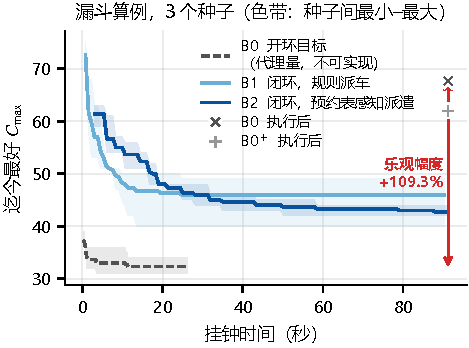
\includegraphics[width=\columnwidth]{fig/fig_convergence_closedloop_CN.pdf}
\Description{Best-so-far makespan against wall-clock time for the ladder
configurations, with the open-loop curve marked as a surrogate objective and its
realizable value shown as a separate point. Each curve carries a shaded band
giving the min-to-max range across the three seeds.}
\caption{单个 \texttt{funnel} 算例上的收敛曲线，横轴为挂钟时间，曲线为多种子的逐时刻均值，
阴影带为种子间的\emph{全距}（本图只有三个种子，四分位撑不起来）。
实线（B1、B2）自始至终是可实现的完工时间；虚线是开环搜索自己的代理目标，即它实际在优化的量；
叉号与十字标出同一份计划经无冲突路由执行后的位置。
虚线终点与叉号之差即该算例的乐观幅度：开环并非收敛得不好，而是收敛到一个不可实现的代理目标。
本图只取三个算例、三个种子，不承载统计主张；本章统计一律以 $\NCases$ 组 $\times$ $\NSeeds$ 个种子的主批次为准。
本图挂钟预算为 $46.3$ 秒，与主批次的 $90$ 秒不同。}
\label{fig:convergence}
%% 由 fig/fig_convergence_CN.py 生成(输出名 fig_convergence_closedloop_CN),
%% 数据源 clbs/output/ladder_convergence.csv 与 ladder_cost.csv,由 tools/ladder_diag.py 落盘。
%% 该图是说明性的:它画形状与落差,不承载统计主张,故只取三算例三种子,正文统计一律以
%% baseline_ladder.csv 为准。此口径已写在 ladder_diag.py 的首部注释里。
\end{figure}

\paragraph{预约表感知派遣。}
固定开环或闭环、只改选车规则。在\emph{闭环内部}，
$\text{B1}\to\text{B2}$ 为 $-\GainProbeLoop$($p\PProbeLoop$)，伪中位数 \HLProbeLoop{}，
$95\%$ 置信区间 \CIProbeLoop{}。
两级的排产搜索与预算相同，只差选车时是否按预约表试算。
这是合计口径：区间不跨零，下端离零不到一个百分点；按族校正后无一组建组显著（校正前为 \CellsSigProbe{} 组），且十组中两组符号为正——车臂比 $1.0$ 与 $2.0$ 上 B2 慢于 B1（表~\ref{tab:main}）。
因此 $-\GainProbeLoop$ 是本算例族上的平均，不是可以逐组兑现的点估计；
第~\ref{sec:whichcongestion}~节说明这一分辨率限制。

在\emph{开环之下}，同一规则为 $-\GainProbeOpen$($p\PProbeOpen$)，同样显著。
它对应~\cite{sun2023integrated} 两阶段结构相对~\cite{li2026framework} 开环的那一段；
量级（\GainProbeOpen{}）远小于闭环（\GainLoopRule{}）。
查预约表选车在开环与闭环下各自显著，但小得多，单独解释不了 $\text{B0}\to\text{B2}$ 的降幅。

\paragraph{端到端。}
$\text{B0}\to\text{B2}$ 合计 $-\GainEndToEnd$
($p\PEndToEnd$，$\NPairs$ 个配对中 $\WinEndToEnd$ 胜 $\LoseEndToEnd$ 负 $1$ 平)。
上面两段已拆开：从开环加规则派车走到闭环加预约表感知派遣，完工时间降低约五分之一。


\subsection{近加性与不可互相替代}
\label{sec:complement}

上一节三笔量级不同。开环下只改选车：$\GainProbeOpen$，显著但小。规则派车下只改搜索是否计入让行：$\GainLoopRule$，显著且大。闭环内部再改选车：合计均值为 $\GainProbeLoop$，其中车臂比 $1.0$ 与 $2.0$ 两组上 B2 慢于 B1，把均值拉低。
本节分开回答两件事：二者可否互相替代，以及是否正交互。

\paragraph{交互。}
若闭环与派遣彼此独立，端到端增益应等于二者单独增益的复合：由规则派车下的闭环（$\GainLoopRule$）与开环下的派遣（$\GainProbeOpen$）得到 $\GainIndepProduct$。
实测为 $\GainEndToEnd$，略低于该预测——\emph{未检出正交互}，呈近加性。二者并不互相放大。

\paragraph{不可互相替代。}
开环下只改选车，不能代替闭环。排产按理想行驶时间确定、只按预约表选车，得到约 $\GainProbeOpen$；搜索时计入让行、仍用规则派车，得到约 $\GainLoopRule$。
同一派遣规则放进~\cite{sun2023integrated} 那种两阶段结构，管用到开环派遣那一档；要拿到闭环这一级的降幅，让行必须在搜索时进入适应度。
B2 仍是端到端最优，因为它把两笔收益叠在一起，不是因为存在正交互。

\paragraph{与「先排产、后解冲突」的关系。}
这条路线的缺口不在第二阶段派车——该阶段在本文口径下确有 $\GainProbeOpen$ 的显著收益——而在第一阶段未计入让行，闭环那一笔进不去。
上述落差是本文算例族上测得的一个点，不是已被证明的界。

\subsection{三族扫描与单组分辨率}
\label{sec:whichcongestion}

第~\ref{sec:main}~节的合计比较建立在 $\NCases$ 组算例上。本节按布局、车臂比与柔性拆开。
闭环可以按族读走势；派遣在单组上分辨不出。这个不对称就是本节要报的。三族各对应一个事先说得清的预期。

\emph{布局（A 族）}检验收益是否随争用强度增长：两条通路处理的都是争用，争用弱则无从发挥。
\texttt{funnel} 与 \texttt{high} 只差站台一条并行通道，最小割减半，是最干净的对照。

\emph{车臂比（B 族）}检验车队规模是否存在收益被开销吞掉的上界。试算开销随车队近似线性增长，第~\ref{sec:speedup}~节的剪枝在最大车队一档削减率最低。
四个水平 $N_A/N_M\in\{0.5,1.0,1.5,2.0\}$，其中 $1.5$ 为共用基点 \texttt{A funnel}。

\emph{柔性（C 族）}检验收益是否依赖改派余地。$F\in\{0.3,0.6,1.0\}$，其中 $0.6$ 同为基点。

\paragraph{单组分辨率。}
表~\ref{tab:bytag} 的显著性标记决定哪些组可以按符号来读。
对 $\NCases$ 组各做一次检验，全零假设下「至少一处显著」远高于 $5\%$。
故逐组检验按族做 Holm 校正，族取一个效应的 $\NCases$ 组（闭环与派遣各成一族；二十次并成一族，等于去校正一个并未做的对比）。
表~\ref{tab:bytag} 与图~\ref{fig:prediction3} 的标记均以校正后的 $p$ 为准。

闭环校正后仍有 \CellsSigLoopAdj{} 组自身显著（校正前 \CellsSigLoop{} 组，校正后最大一处 $p\PLoopCellMax$，判定不依赖于是否校正）；唯一例外是车队最紧的一组（$\text{B0}\to\text{B1}$ 为 \GainLoopStarve{}，不显著）。故闭环可以按族读走势。
闭环内派遣校正前有 \CellsSigProbe{} 组显著（柔性族两端，$p\PProbeFlexLoRaw$ 与 $p\PProbeFlexHiRaw$），\emph{校正后为 \CellsSigProbeAdj{} 组}：Holm 后为 $p\PProbeFlexLoHolm$ 与 $p\PProbeFlexHiHolm$，Benjamini--Hochberg 为 $p\PProbeFlexLoBH$ 与 $p\PProbeFlexHiBH$，同样不显著。
没有任何一组可以单独站住。其量级（数个百分点）与单组 $\NSeeds$ 个种子所能分辨的下限同阶，只有合计 $\NPairs$ 个配对才把它抬出噪声；即便合计也只是刚过：伪中位数 \HLProbeLoop{}，$95\%$ 区间 \CIProbeLoop{}，不跨零，下端离零不到一个百分点。
下文对派遣的逐组读数只作方向，不作结论；符号判断只在合计口径上给出。

\begin{table}[t]
\caption{逐组的四级阶梯结果与闭环、派遣两个效应，按三族分块（每组 $n=\NSeeds$ 个按种子配对的比较）。
显著性标记按 \textbf{Holm 校正后}的 $p$ 给出（双侧 Wilcoxon 符号秩检验），族为一个效应的
$\NCases$ 组：$^{*}p<0.05$、$^{**}p<0.01$；$^{\dagger}$ 表示校正前显著、校正后不显著，该组符号不作结论。
争用强度由算例结构读出。负值表示完工时间下降。两个增益列与表~\ref{tab:main} 同一估计量（逐对相对增益在种子上的均值），十组均值在舍入误差内等于该表合计（逐位复算用未舍入值）；该列不能由同行两个均值相除反推。
\texttt{A funnel} 同时是 B 族 $N_A/N_M=1.5$ 与 C 族 $F=0.6$，只运行一次，只列一行。}
\label{tab:bytag}
\small
%% 由 tab/gen_tables_ladder.py 生成,按 A/B/C 三族分块。
%% 逐格增益列已于 2026-08-16 从"两档均值之比"改为"逐对相对增益的均值",与 tab_main 及
%% 导言区宏同源;同时加印显著性标记,因为下文按格读符号。
%% 标记已于 2026-08-20 改按 Holm 校正后的 p 值,并为"校正前显著、校正后不显著"的格加印
%% 剑号。改动只影响标记,不影响任何增益数字;受影响的格是柔性族两格(试探列)。
%% generated by tab/gen_tables.py -- do not edit by hand
\begin{tabular}{@{}lccccc@{}}
\toprule
& \multicolumn{4}{c}{$\Delta C_{\max}$ (\%) at $H=$} & pooled \\
\cmidrule(lr){2-5}
Structure & $0$ & $0.15$ & $0.3$ & $0.5$ & (\%) \\
\midrule
\texttt{low} & $+10.3$ & $+5.6$ & $+8.8$ & $+10.4$ & $+8.76^{***}$ \\
\texttt{mid} & $+3.3$ & $+4.0$ & $+4.5$ & $+4.3$ & $+4.03^{***}$ \\
\texttt{high} & $+11.3$ & $+8.1$ & $+10.7$ & $+7.9$ & $+9.50^{***}$ \\
\texttt{funnel} & $+9.2$ & $+8.7$ & $+9.4$ & $+6.5$ & $+8.47^{***}$ \\
\bottomrule
\end{tabular}

\end{table}

\begin{figure}[t]
\centering
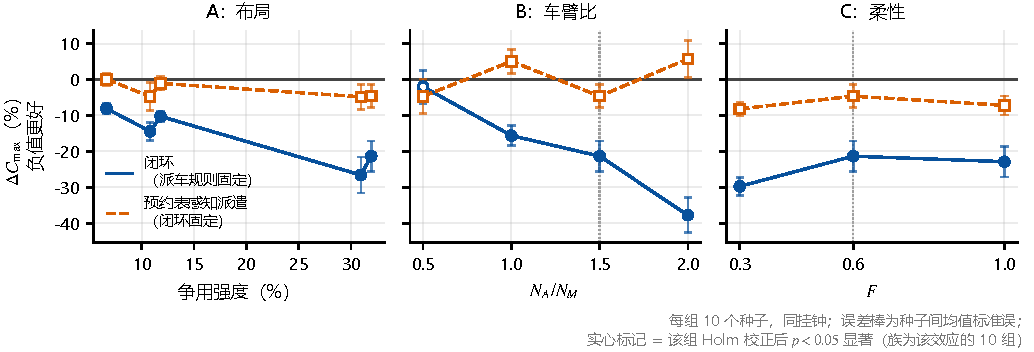
\includegraphics[width=\columnwidth]{fig/fig_prediction3_CN.pdf}
\Description{Three panels of line plots: closed-loop gain and reservation-aware
dispatch gain across layout (vs contention), fleet-to-arm ratio, and flexibility. After
Holm correction over the ten cells the closed-loop curve is filled, hence
significant, at nine of ten cells, while the dispatch curve is hollow at every
cell, and its sign alternates across the four fleet-ratio levels. Error bars
give the standard error of the mean over the ten seeds of each cell; the
dispatch bars cross zero at every cell and the closed-loop bars do not.}
\caption{闭环与派遣在三族上的分布。左：布局族，横轴为争用强度；中：车臂比，$N_A/N_M$；右：柔性。
B、C 两族含共用基点（空心竖线处的 $1.5$ 与 $0.6$），同时列于 A 族 \texttt{A funnel}。
实心为 Holm 校正后仍显著（$p<0.05$，族为一个效应的 $\NCases$ 组），空心为不显著。
误差棒为该组 $\NSeeds$ 个种子上逐对相对增益的均值标准误。
闭环 \CellsSigLoopAdj{} 组显著，大体随争用上升；派遣校正后\emph{无一显著}，误差棒逐组跨零，车臂比四个水平上符号还交替。
本图要读的是两条曲线能否与零区分，不是派遣那条曲线的形状。}
\label{fig:prediction3}
%% 由 fig/fig_prediction3_CN.py 从 clbs/output/baseline_ladder.csv 生成。横轴:A 族取争用强度
%% (布局族没有自然的数值水平,而布局操纵改变的正是争用),B/C 族取算例名末尾的因子水平——
%% 那个数字由 tools/abc_matrix.py 生成算例时写入,故按构造即为水平本身;基点 A funnel 的
%% 名字里没有水平,其 (1.5, 0.6) 由脚本按 abc_matrix.BASE 显式补入,见脚本内注释。
%% 标记的实心/空心由逐格 Wilcoxon 的 p 值决定。上一版按增益是否为正标注 "harmful",
%% 那等于把不显著的符号当成结论,现已改为按显著性区分标记。
%% 2026-08-20:填充判据改为 Holm 校正后的 p 值,族取该效应的全部十格(而不是当前面板的
%% 三到五格,否则共用基点会因所在面板不同而得到两种填充)。改动后试探那条曲线全为空心。
\end{figure}

表~\ref{tab:bytag} 与图~\ref{fig:prediction3} 给出逐组结果。三族读法不同。

\emph{布局族。}
闭环随争用强度大体上升，五组均显著：最不拥堵的 \texttt{scatter}（争用 \ContentionLo{}）上 $\text{B0}\to\text{B1}$ 为 \GainLoopScatter{}，\texttt{mid}/\texttt{low} 为 \GainLoopMid{}/\GainLoopLow{}，\texttt{funnel}/\texttt{high} 为 \GainLoopFunnel{}/\GainLoopHigh{}。
「大体」是因为有两处逆序，性质不同。
\texttt{low} 争用高于 \texttt{mid} 而收益更小，跨过第~\ref{sec:instances}~节的拓扑分界（网格对哑铃，最远行程 \LegGrid{} 对 \LegDumbbell{}），不是单纯的争用逆序。
\texttt{funnel} 争用高于 \texttt{high} 而收益更小：同为哑铃、只差站台一条并行通道，这是指定的最干净对照，\emph{这一处才是反例}。
能说的是量级——最拥堵一组 \GainLoopFunnel{} 对最不拥堵一组 \GainLoopScatter{}，约两倍半——不是争用对收益的单调排序。
争用强度把拥堵压成一个数，不区分其中有多少可由改派绕开；第~\ref{sec:limitations}~节局限 (1)。
派遣在本族逐组均不显著，只记方向：五组中四组为负，与闭环同向。

\emph{车臂比族。}
原拟用来钉适用上界，钉不下来。闭环内派遣四个水平依次为 $-\GainProbeStarve$（$N_A/N_M=0.5$）、\GainProbeFleetOne{}（$1.0$）、\GainProbeFleetBase{}（$1.5$，基点 \texttt{A funnel}）、\GainProbeFleetTwo{}（$2.0$）：符号交替，四组无一显著（$p\PProbeFleetHalfRaw$、$p\PProbeFleetOneRaw$、$p\PProbeFleetBaseRaw$、$p\PProbeFleetTwoRaw$；这四个是校正\emph{前}的值，连未校正阈值都够不到）。
若只取 $0.5$、$1.0$、$2.0$，曲线像代价律所预言的单调上升，前一版据此写过「$N_A/N_M\ge 1$ 即为适用上界」；补回中间的基点后，这条叙事不成立。
效应与单组噪声同阶时，\emph{子集选取本身就能造出一条趋势}；防住它的办法是把扫描补全并逐组检验。
第~\ref{sec:costlaw}~节所预言的上界因此仍是未检验的预言：要检验它，种子数须高到能分辨数个百分点，超出本文预算。
闭环在 $1.0$ 与 $2.0$ 上为 \GainLoopFleetOne{} 与 \GainLoopFleetTwo{}，均显著：车队变大，主要改变的是闭环能降多少，不是派遣。

\emph{柔性族。}
原拟作为派遣唯一能作结论的一族，Holm 校正后撤回。
$F=0.3$、$0.6$、$1.0$ 上派遣为 \GainProbeFlexLo{}、\GainProbeFleetBase{} 与 \GainProbeFlexHi{}：三者同号，两端是全部 $\NCases$ 组中量级最大的两组（基点回落到与其余相当）；两端 $p\PProbeFlexLoRaw$、$p\PProbeFlexHiRaw$ 校正后升至 $p\PProbeFlexLoHolm$、$p\PProbeFlexHiHolm$，已不显著。
本族只提供与合计同向、量级最大的方向性证据。
三个水平上同号、没有车臂比那种符号交替，与「走廊争用主要经选车与时序调整，并不强依赖还有没有另一台臂」相容：若它只是柔性车间的旁路，$F=0.3$ 本该最先失效，而它恰是量级最大的一组。相容不等于证实。
闭环为 \GainLoopFlexLo{} 与 \GainLoopFlexHi{}，校正后仍逐组显著。

\paragraph{另一批自建算例。}
上述读数来自一个算例族、一种基线。交叉核对用另一批仍带争用的自建算例（公开基准见第~\ref{sec:external}~节，那里争用已删去）：$\MatrixCells$ 组 $\times$ $10$ 种子，共 $\MatrixRuns$ 次运行。
算例核心与基线均不同：基线为两阶段代理运输，并在四个争用水平与四个异构度水平上交叉。
预算与种子也不同：挂钟按算例标在 $30.2$ 至 $72.9$ 秒（批次内各配置共享同一标定，故配置之间仍是同预算），种子另取十个。
\emph{集成增益}（两阶段 $\to$ 闭环）为 \GainIntegMatrix{}，$\MatrixCells$ 组中 \SigIntegMatrix{} 组显著，区间 \GainIntegMatrixLo{} 到 \GainIntegMatrixHi{}，与本章闭环的方向和量级一致。
凡引这批数据的显著组数，均为该批报表的\emph{未校正}计数（第~\ref{sec:protocol}~节第二处例外），只作方向与量级印证，不作逐组断言。

\paragraph{异构度没有抬高闭环收益。}
该批四个 $H$ 水平回答第~\ref{sec:instances}~节留下的问题。按 $H$ 把 $\MatrixCells$ 组分成四档（每档 $4$ 组，四个争用水平各一），集成增益为：$H=0$ 时 \GainIntegHZero{}，$H=0.15$（实测 \MatrixHMeasLow{}）时 \GainIntegHLow{}，$H=0.3$ 时 \GainIntegHMid{}，$H=0.5$ 时 \GainIntegHHigh{}；增益与 $H$ 的秩相关为弱负的 \RhoIntegH{}。

实测 $H=\MatrixHMeasLow$ 落在公开算例中位 \PubHMed{} 附近，其 \GainIntegHLow{} 与 $H=0.3$ 的 \GainIntegHMid{} 相差不到半个百分点：把 $H$ 定在文献区间之上，并未抬高闭环收益。
收益随 $H$ 上升这一预期不成立——趋势非单调，秩相关为负。每档只有 $4$ 组，组内散布（\GainIntegMatrixLo{} 到 \GainIntegMatrixHi{}）远大于档间差距，故只支持「收益不随 $H$ 上升」，不足以断言 $H=0.5$ 更低。
与第~\ref{sec:features}~节的定义相容：$H$ 增大时，可选臂之间的工时差异逐渐压过走廊可达性差异，指派越来越由哪台快决定、越来越少由哪条路不堵决定。
$H=0$ 关闭的是权衡，不是机会：$\Omega_{ji}$ 内各臂工时相同，改派不必用加工时间换通行时间，成为代价为零的纯拥堵决策；该档增益居四档之首（\GainIntegHZero{}），与定义一致。
因此 $H$ 使「选哪台臂」成为一个权衡——没有它，第~\ref{sec:Chapter_I}~节的反转无从谈起——但不是闭环收益的放大器。闭环收益来自搜索时是否计入让行；争用强弱由布局与车队决定，不由 $H$ 决定。

该批对预约表感知派遣给出 \GainProbePre{}，$\MatrixCells$ 组中 $0$ 组显著，与本章 $\GainProbeLoop$ 方向相反。成因确定：该批运行于第~\ref{sec:speedup}~节两项加速之前，当时同一规则的开销尚未压下来。

\subsection{消融与受控负对照}
\label{sec:pricing}

第~\ref{sec:interface}~节列出层间接口的三种选择。默认配置只用第一种（预约表感知派遣）；另外两种均已实现并度量，同挂钟下都没有净收益。本节报告这些测量。

\subsubsection{按让行记录的局部搜索}
在第~\ref{sec:whichcongestion}~节那批 $\MatrixCells$ 组数据中，关掉让行记录反馈的相对增益为 \GainCertMatrix{}（$\MatrixCells$ 组中仅 $1$ 组显著），关掉错峰算子为 \GainStaggerMatrix{}（$2$ 组显著）。两者都不为正：同挂钟下，把解码次数花在这个邻域上，不如还给种群循环。机制解释见第~\ref{sec:whycost}~节。

这两项消融可以引用该批更早的数据，派遣的消融不可以：让行记录与错峰在两项加速前后没有改动，开销也不随剪枝变化；派遣的开销正是加速所针对的对象。

\subsubsection{走廊时段附加代价}
第~\ref{sec:interface}~节指出：对已占用走廊时段再附加代价，等于把适应度已经计入的延误数第二遍。该论证说明加价不增加信息，但不给出完工时间变差有多大。二者须分开测。
在两种预算口径下扫描 $\theta$，并在所有 $\theta$ 上固定路径规划的搜索宽度，以免把加价与「考察多少个进入时刻」混在一起。

\begin{figure}[t]
\centering
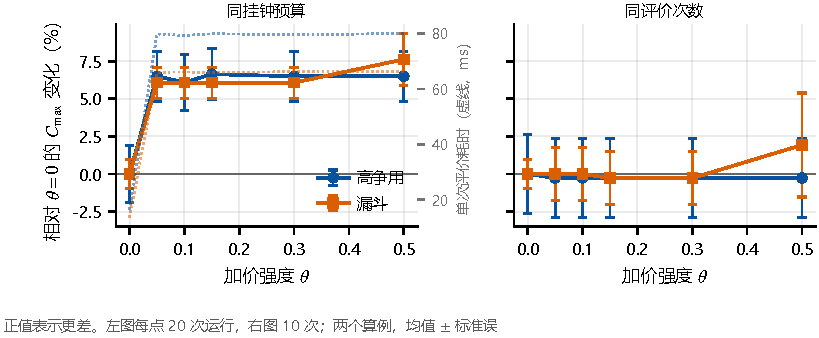
\includegraphics[width=\columnwidth]{fig/fig_theta_CN.pdf}
\Description{Two panels of makespan change relative to theta equals zero against
pricing strength: under equal wall-clock the penalty is large and flat, under
equal evaluations it is absent. Markers are means over seeds and error bars are
the standard error of the mean. The batch is two separately generated instances
that are not members of the paper's A/B/C families.}
\caption{走廊时段附加代价。正值表示更差。同挂钟（左）下，完工时间变差在加价一开启即出现，随后在 $\theta$ 的十倍范围内平坦，并与右轴的单次评价开销同步；同评价次数（右）下变差消失。
损害来自单次评价开销升高、同一预算内评价次数减少，不是价格把路径选错。
标记为均值，误差棒为均值标准误，每点运行次数标在图内页脚；「显著」指每个 $\theta$ 与 $\theta=0$ 按种子配对的双侧 Wilcoxon 符号秩检验。
本图为两个 $8$ 工件 $\times\,4$ 机器 $\times\,4$ 车的算例，\emph{不属于}表~\ref{tab:instances} 的 A/B/C 三族（后者一律 $12\times 8\times 12$）；图例 \texttt{high}/\texttt{funnel} 只是布局标签，与 A 族同名两组并非同一算例。
左图 $10$ 个种子、右图 $5$ 个（前者的子集），挂钟分别为 $48.9$ 秒与 $60.7$ 秒，均不同于主批次的 $90$ 秒。
该批采集于第~\ref{sec:speedup}~节两项加速\emph{之前}；加价机制在加速前后未改动，开销与剪枝无关（剪枝作用于派车试算，不作用于多标签路由），故对本节判断仍有效，但不能与本章其余各表逐组并列。}
\label{fig:theta}
%% 由 fig/fig_theta_CN.py 从 clbs/experiments/theta_sweep.csv 与 theta_sweep_gen.csv 生成
%% (08-05 落盘,2 算例 x 10 种子,左图每点 20 次运行、右图 10 次)。
%% 更正:先前此处标注为"数据未落盘",实为误记——两个 CSV 均在盘上,已重新出图核对,
%% 图上形态与本小节正文一致(同挂钟下每个 theta 都变差且在十倍范围内平坦,同评价次数下归零)。
%% 该批次同属降本之前的测量,与第 5.5 小节引用的矩阵批次同期;定价机制在降本前后未改动,
%% 且其开销与剪枝无关(剪枝作用于派车试探,不作用于多标签路由),故该测量对它依然有效。
\end{figure}

实测见图~\ref{fig:theta}。同挂钟下，试过的每个 $\theta$ 上都使完工时间变差且显著，变差在 $\theta$ 的十倍范围内平坦；同评价次数下，同一比较与零无法区分。
带附加代价的路由在同一预算内完成的评价次数约为不加价时的五分之一：加价没有把候选解排错序，而是让同一预算内少评了许多次。

另外两点排除别的读法。其一，$\theta$ 在本问题上不是有用的旋钮：跨两个数量级，带价路由改的是同样几条路径、付同样的总价、返回同样的完工时间；累计价格只占总行驶时间的很小一部分，不足以推翻 $\text{到达时刻}+\theta\cdot\text{价格}$ 里到达时刻的次序。只有 $\theta$ 大到价格压过到达时刻，双重计价才显出来，那时完工时间大幅恶化。
其二，开销是结构性的，不是价格非零造成的：同一次解码带价与不带价的耗时之比在每个 $\theta$ 上都相同——付的是「每个节点维护 Pareto 前沿、每条弧尝试若干进入时刻」，与是否真的加价无关。这正是引理~\ref{lem:label} 所说的：引入第二判据即不再能全序占优，单标签搜索必须换成多标签搜索。

两种预算口径对幅度有分歧，对符号没有。与实现无关的部分是：无论价格来自走廊容量的有限差分还是关键链代理，收取的都是一笔后果已在让行车辆到达时刻里付过的占用费。只要适应度取自完整无冲突解码，让行已被计入，再加的价是惰性的；比较结果于是由「为这个惰性信号配备多标签搜索」的开销决定。
因此，在加厚层间接口之前，先看接收层的目标是否已经包含该接口要传的量；若已包含，在本文口径下这种加厚有害。

%% 由独立小节降为上一节的子小节:它是消融的机制解释,不是本文的一级结论。
\subsubsection{稀释与开销}
\label{sec:whycost}

让行记录与错峰未能抵偿开销，原因可以测出来；同一测量也说明预约表感知派遣为何必须先压低开销。

\paragraph{解码次数用在何处。}
按让行记录的局部搜索消耗了全部解码次数中的很大一部分，而所解码的邻居里，能改进完工时间的比例低于五十分之一。改进本身是真实的；同样这些次数还给种群循环，产出更多。

低命中率不是实现缺陷。该邻域按构造既小又有指向（第~\ref{sec:ls}~节）；有指向而仍低命中，说明记录所指的那些工序，改派或错峰之后并不能缩短关键链。
试过三种修补：按路径上的预期让行而非理想距离为改派打分、把错峰的相邻交换换成定向插入、以及接受「完工时间不变但总让行下降」的平台移动。每一种都在同评价次数下与未改算子独立比较，\emph{无一}显著。失效在信号，不在如何使用信号。

\paragraph{沿关键链的稀释。}
一份让行记录指明某次让行的走廊、时段与先行占用该走廊的运输，这是消除\emph{那一次}事件所需的信息。
完工时间经由一条链达成，去掉一处走廊延误通常会把另一约束顶成紧约束——某道上游工序、某台机械臂、或另一条走廊——实现的改进只是被消除延误的一个分数。
接受准则在每次接受后重新提取关键链，正出于此。当瓶颈只是若干量级相当的瓶颈之一时，能指名瓶颈的反馈，其作用远小于该次让行的时长。

\paragraph{派遣在加速前后为何一正一负。}
上一小节的摊薄同样作用于预约表感知派遣：试算选出的是当前任务送达最早的车，这是局部改进；完工时间还要经过整条关键链，实现的降幅只是其中一部分。
摊薄之后这笔降幅仍为正，但只有数个百分点。加速之前，单次评价开销是规则派车的 \CostMultBefore{} 倍，同一挂钟内评价次数不够，净效果落进噪声（第~\ref{sec:whichcongestion}~节那批数据）。
第~\ref{sec:speedup}~节把开销压到 \CostMultAfter{} 倍之后，同一笔降幅才在合计口径上显著。

固定预算下要同时看两件可以分开测、分开改的量：摊薄之后还剩多少完工时间降幅，以及每次评价多花多少。
二者不是一起坏。按让行记录的局部搜索，问题在前一件：摊薄后剩下的降幅太小，改邻域的三种修补在同评价次数下都没有做到显著。
派遣的问题在后一件：摊薄后的降幅本来就在，起初不显著是因为单次评价开销过高；这笔开销可以在不改变所选车辆与时间表的前提下压低。
所以默认配置保留派遣，不用让行记录去生成邻域。


\subsection{代价律与降本效果}
\label{sec:costlaw}

单次评价开销与评价次数是同一段挂钟的两种花法。同一派遣规则在加速前净效果落在噪声里，加速后显著为正，故把二者本身测出来。

\paragraph{两种预算口径。}
图~\ref{fig:protocol} 给出各配置的单次评价开销，以及同一预算上限内实际完成的评价次数。开销跨越约两个数量级：开销更低的配置完成更多评价，开环用掉不到两成挂钟就完成了最多的评价次数。
按相同代数比较，等于让开销更高的配置多占用算力；对齐挂钟则让开销更低的配置多评许多次。两种口径都不单独呈现。

\begin{figure}[t]
\centering
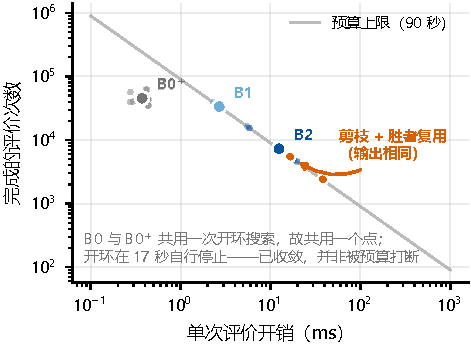
\includegraphics[width=\columnwidth]{fig/fig_protocol_CN.pdf}
\Description{A log-log scatter of cost per evaluation against evaluations
completed. A grey hyperbola marks the 90-second budget cap. The two closed-loop
configurations sit on it, while the open-loop configuration sits well below it
because it stalls after about seventeen seconds. An arrow shows the pruning
ablation moving one configuration along the line without changing its output.}
\caption{固定挂钟预算把单次评价开销与完成的评价次数锁成一条双曲线；灰线为各档共享的 $90$ 秒上限。
贴在线上，表示开销 $\times$ 次数等于该档挂钟。两个闭环配置贴在线上——每一次都跑满预算；开环落在线\emph{下方}，因为约四百余代后不再改进而自行停止，约 $17$ 秒即收敛，并非被预算打断（第~\ref{sec:protocol}~节）。
B0 与 B0$^+$ 共用同一次开环搜索，故共用一个点，差别只在执行方式。淡色小点为三个算例的逐个读数，实心大点取其几何平均：对数轴上只有几何平均保持「开销 $\times$ 次数 $=$ 该档挂钟」。
橙色箭头是剪枝与胜者路径复用的开关两档——命题~\ref{prop:speedup_equiv} 保证\emph{不改变输出}即可沿该线移动，故这段位移只是算力节省。}
\label{fig:protocol}
%% 由 fig/fig_protocol_CN.py 生成(输出名 fig_protocol_CN),数据源 clbs/output/ladder_cost.csv
%% 与 prune_ablation.csv;后者缺失时脚本自动省略橙色箭头而不报错。
\end{figure}

图~\ref{fig:protocols} 把同一组比较在两种口径下各做一遍。同代数不为多出的单次开销付费，因而偏袒单次评价开销更高的配置：预约表感知派遣相对规则派车为 \GainProbeSameGen{}（$p\PProbeSameGen$）；同挂钟下、加速之前，同一比较只剩 \GainProbeSameClock{}（$p\PProbeSameClock$），几乎归零。
同代数问的是：多做的那步路由有没有改进这一代的排序；同挂钟问的是：同一段时间里完工时间有没有降。两问都成立，但不能把其中一个报成另一个。

\begin{figure}[t]
\centering
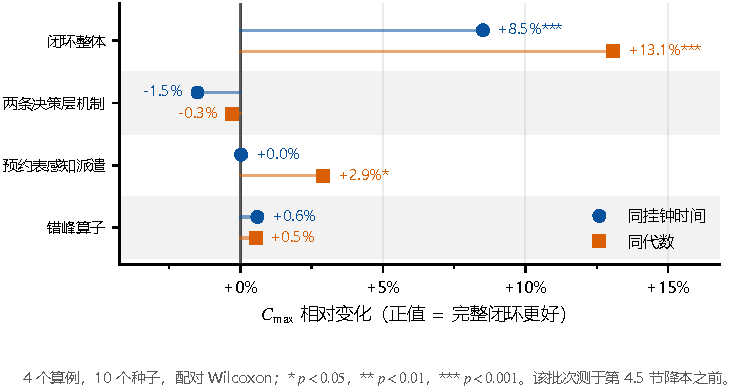
\includegraphics[width=\columnwidth]{fig/fig_protocols_CN.pdf}
\Description{The same paired comparisons shown twice, once under an equal
wall-clock budget and once under an equal number of generations.}
\caption{同一组比较在两种预算口径下的读数。每一行按它所隔离的机制命名，不按配置对命名。
两标记之差来自口径：预约表感知派遣在同代数下为 \GainProbeSameGen{}（$p\PProbeSameGen$），同挂钟下降到 \GainProbeSameClock{}（$p\PProbeSameClock$），即归零。
该批运行于第~\ref{sec:speedup}~节两项加速\emph{之前}，故这一行也是下文只动加速的对照的动机。}
\label{fig:protocols}
%% 由 fig/fig_protocols_CN.py 从 clbs/experiments/protocols.csv 生成(4 算例 x 10 种子)。
%% 行标签已从旧叙事的档位名(two-stage / open dispatch ...)改写为它所隔离的机制名,
%% 以免读者以为该图来自另一项研究;图脚已自报"降本之前"这一批次归属。
\end{figure}

\paragraph{代价律。}
预约表感知派遣把每个运输任务的路由调用从 $2$ 次升到至多 $2N_A$，开销随车队规模线性增长。
剪枝所用下界在争用越弱时越紧，跳过的候选越多；车队越大、争用越强，削减越少。
第~\ref{sec:speedup}~节的等价性自检给出这个方向：六组中调用削减率最高的是最不拥堵的一组（\RouteCallCutHi{}），最低的是车队最大的一组（\RouteCallCutLo{}）——是效力衰减，不是失效。
两趋势合在一起\emph{预言}：车队足够大且争用足够强时，试算开销的增长会追上收益。这仍是预言。第~\ref{sec:whichcongestion}~节车臂比四个水平上符号交替，四组无一显著，没有证实这条上界。
代价律本身（开销随 $N_A$ 线性、剪枝效力随 $N_A$ 下降）是直接测得的；由它推出的上界不是。前一版把前者当作后者的证据，不成立。

\paragraph{只开、关两项加速。}
加速与派遣规则是先后引入的，并列两个批次无法排除算例与基线不同。因此做一档只动加速的对照：同算例、同种子、同预算，只开或关剪枝与胜者路径复用。

命题~\ref{prop:speedup_equiv} 保证两项优化\emph{不改变输出}。六个算例上各取六条随机染色体，两档的完工时间与派车序列\emph{逐位相同}，共 $36$ 组无一例外；路由调用合计减少 \RouteCallCut{}。输出既已相同，关掉优化只会使单次评价变慢，同挂钟下的完工时间差就\emph{只}来自省下的算力。

表~\ref{tab:prune}：关$\to$开使完工时间再降 \GainPrune{}（\WinPrune{} 胜 /\LosePrune{} 负，$p\PPrune$），同预算内评价次数为 \EvalRatioPrune{} 倍，单次评价加速 \SpeedupProbe{} 倍。
由此接上两个批次：同一规则在加速前的矩阵批上为 \GainProbePre{}（$\MatrixCells$ 组中 $0$ 组显著），加速后的阶梯批上显著为正；中间这一步没有改变任何一个选择。

\begin{table}[t]
\caption{只改变剪枝与胜者路径复用。"关"/"开"指二者是否启用，加粗表头为本文采用的一档。
两档输出逐位相同（已过等价性自检），故差值只来自省下的算力。同算例、同种子、同挂钟；$n=60$ 配对，双侧 Wilcoxon 符号秩检验（$^{***}p<0.001$），合计行并列胜/负/平与 $p$。
两个比值列的分母都是\emph{关}档，方向相反：评价次数按 开/关，单次评价耗时按 关/开。}
\label{tab:prune}
\small
%% 数字与 clbs/output/prune_ablation.csv / 运行日志一致;亦可用
%% py paper01/tab/gen_tables_ladder.py 从同一 CSV 重生成。
%% 由 prune_ablation.csv 汇总写入(与 tools/prune_ablation.py 日志一致),勿手工改数字
%% 6 算例 x 10 种子;开=exact(剪枝+复用),关=exact_noopt;输出逐位相同
\begin{tabular}{@{}lrrrrrr@{}}
\toprule
算例 & 争用强度 & 关 & 开 & $\Delta C_{\max}$ & 评价次数比 & 加速比 \\
\midrule
A funnel & 31.9\% & 44.80 & \textbf{42.10} & $-6.03\%$ & 2.21$\times$ & 2.23$\times$ \\
A high & 30.9\% & 41.60 & \textbf{37.70} & $-9.37\%$ & 2.40$\times$ & 2.41$\times$ \\
A low & 11.8\% & 60.50 & \textbf{57.00} & $-5.79\%$ & 2.79$\times$ & 2.81$\times$ \\
B NA/NM 0.5 & 15.8\% & 66.70 & \textbf{65.10} & $-2.40\%$ & 2.11$\times$ & 2.11$\times$ \\
B NA/NM 1.0 & 30.2\% & 51.90 & \textbf{48.90} & $-5.78\%$ & 2.31$\times$ & 2.31$\times$ \\
B NA/NM 2.0 & 32.4\% & 44.50 & \textbf{42.20} & $-5.17\%$ & 1.98$\times$ & 2.01$\times$ \\
\midrule
\emph{配对合计}(60 配对) & --- & --- & --- & $-5.60\%^{***}$ &
\multicolumn{2}{r}{50/0/10,\ $<10^{-4}$} \\
\bottomrule
\end{tabular}

\end{table}

\subsection{案例：漏斗算例上的甘特图与关键链}
\label{sec:casestudy}

合计数字不显示一次求解里发生了什么。本节在单个漏斗算例上并排 B0 与 B2，并按表~\ref{tab:attrib} 给关键链各节着色。

图~\ref{fig:case_gantt} 把机械臂与车辆画在同一时间轴上；车辆行区分空载、满载，让行单独着色。可以直接读出三点。开环解里，让行成段出现在站台附近的走廊上，并集中在少数几辆车上。闭环解把这些等待大幅削去，若干道工序被指派到并非最快的机械臂。闭环解的车辆忙闲也更均衡——这是前两点的结果，不是第三条机制：解里出现了 \eqref{eq:reassign} 那种用较长加工换较短、更好走路程的指派。

\begin{figure*}[t]
\centering
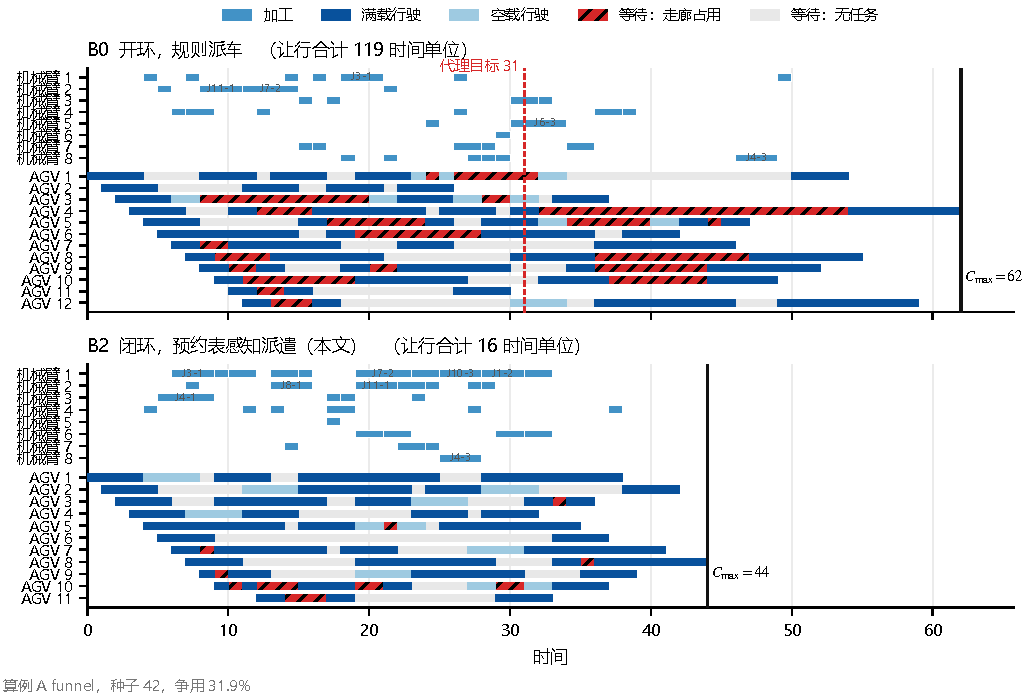
\includegraphics[width=\textwidth]{fig/fig_case_gantt_CN.pdf}
\Description{Side-by-side Gantt charts of the open-loop and closed-loop
solutions on one funnel instance, with arms and vehicles on a shared time axis
and yielding waits shaded separately.}
\caption{同一漏斗算例上 B0（上）与 B2（下）。机械臂与车辆共用时间轴；车辆行区分空载、满载，以及两类空隙。
同一运输任务两段之间的空隙：车被已占用的走廊拦在停靠位上，即让行，也就是本文处理的那种延误。
不同任务之间的空隙：车无活可干。二者分色，以免把空闲读成让行。}
\label{fig:case_gantt}
%% 由 fig/fig_case_gantt_CN.py 从 clbs/output/case_study/*.json 生成(tools/ladder_diag.py
%% 的 --case-study 落盘)。让行/空闲的区分由脚本从相邻段的 task 字段推出,不是另存的标注。
\end{figure*}

图~\ref{fig:case_chain} 把每一节按表~\ref{tab:attrib} 的五类标注着色。B0 的链上 \texttt{corridor} 占显著比例；B2 上它们大体消失，顶上来的是 \texttt{machine} 与 \texttt{upstream}。
这就是第~\ref{sec:whycost}~节所说的摊薄：去掉一处走廊延误，另一个约束成为紧约束。

\begin{figure}[t]
\centering
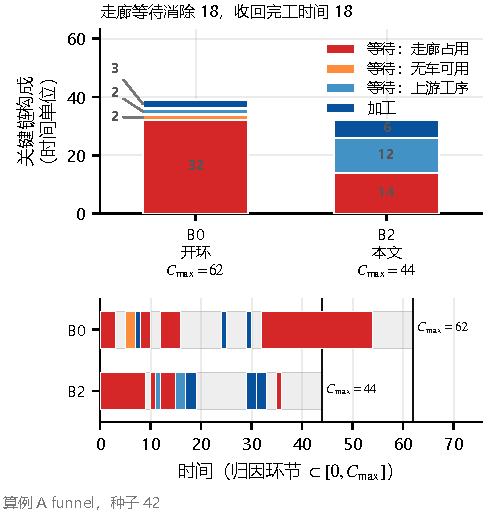
\includegraphics[width=\columnwidth]{fig/fig_case_chain_CN.pdf}
\Description{The critical chain of the open-loop and closed-loop solutions,
with each link coloured by its attribution label.}
\caption{关键链各节按表~\ref{tab:attrib} 着色。上：两档关键链的构成；标题并列「被消除的走廊等待」与「实际收回的完工时间」，二者之差即被顶上来的约束吸收掉的部分。
下：同一条链在时间轴上的原位，表明上方的柱是一条链的分解，不是互不相关事件的直方图。
闭环解中 \texttt{corridor} 大体消失，顶上来的是机械臂与上游工序。}
\label{fig:case_chain}
%% 由 fig/fig_case_chain_CN.py 从同一批 case_study/*.json 生成;归因标签直接取
%% algorithm/decoder.py 的 critical_chain(),五类标签一个不并、不归入 other。
\end{figure}

\subsection{公开基准上的退化比较}
\label{sec:external}

此前各节都是同一套代码的不同配置在自建算例上相比，排除了配置之间的实现差异，但标定不了这套实现的绝对水平：上层搜索若弱，配置之间的差值仍可信，绝对完工时间却只反映实现。本节用公开基准标定上层搜索。

\paragraph{比较什么。}
删去排他约束~\eqref{eq:excl} 之后，本文模型精确退化为标准 FJSP\_PT（第~\ref{sec:Chapter_III}~节），与公开基准是\emph{同一个数学问题}。另取 $\delta_{\mathrm{ret}}=0$ 以对齐这批算例的完工时间定义；它本是模型参数（表~\ref{tab:notation}），不是再删一条约束。
退化后没有走廊争用，两条机制都不进入，检验的是\emph{上层搜索}，不是本文框架。结果与自建算例分表报告，以免两条结论共用一张表。

\paragraph{算例与口径。}
取 Homayouni 与 Fontes~\cite{homayouni2021production} 整理的 \PubNInst{} 个算例（源自 Fattahi 等~\cite{fattahi2007mathematical}，$2$--$12$ 个工件、$4$--$48$ 道工序、$2$--$8$ 台机器），按文献取两辆车~\cite{lim2023twophase}、成品不回运。行驶时间\emph{原样}用所发布的矩阵，不做最短路合成：第~\ref{sec:instances}~节已说明其中 \PubNLayoutBad{} 个矩阵不是任何图的最短路闭包，合成会改算例。
退化之后路网 $G$ 只通过 $t^{*}$ 进入模型，故可把发布矩阵直接当作 $t^{*}$，不必存在与之一致的 $G$。争用需要的是 $G$ 本身，而这批算例没有，故\emph{只能}用在退化档。
两个算例逐位手算核对：$\mathrm{SFJST}01$ 的文献最优值 $70$ 等于站台到机器行程 $4$ 加两道工序 $45+21$；$\mathrm{SFJST}03$ 的 $223$ 等于某台机器上三道工序的紧密排列。两者都不含回运；若计入回运，前者应为 $78$。
参照值：\PubNOpt{} 个算例有 MILP 证明的最优值~\cite{homayouni2021production}，其余 $4$ 个取已发表最好值~\cite{lim2023twophase}。

\paragraph{结果。}
表~\ref{tab:external} 为 \PubNInst{} 个算例 $\times$ \NSeeds{} 个种子。全部 $200$ 次运行通过三条检查：没有低于复合下界的解，没有校验失败；在有可证最优值的 \PubNOpt{} 个算例（$160$ 次运行）上，没有任何一次低于该值。退化档与文献是同一问题，可证最优值是硬下界：若低于它，是转换或口径出错，不是结果更好。
$\PubNMatch{}/\PubNInst{}$ 个算例上最优解与参照值\emph{逐位相同}，其中 $10$ 个小型算例（\textsc{sfjst}01--10）全部命中；\PubNInst{} 个算例平均间隙 \PubGapMean{}（中位 \PubGapMed{}）。
间隙随规模上升，但并非逐个算例单调：\textsc{mfjst}03 与 \textsc{mfjst}06 都优于各自更小的邻居。四个最大算例（$32$--$48$ 道工序）均值为 \PubGapBig{}，最差 \PubGapMax{}；不超过 $24$ 道工序的 $16$ 个算例无一超过 $5.45\%$。

\begin{table}[t]
\caption{公开基准上的退化比较（删去排他约束，与文献同一问题）。「参照」列的
\textsc{opt} 为 MILP 证明的最优值、\textsc{bk} 为已发表最好值；间隙以 \NSeeds{} 个种子的最优
解计。星号标出最优解与参照值逐位相同者。数据：\texttt{experiments\_database/gap\_ideal.csv}。}
\label{tab:external}
\centering
\small
%% 由 tab/gen_tables_ladder.py 生成,请勿手工编辑
%% 数据源:clbs/experiments_database/gap_ideal.csv;工序数取自 clbs/database/json/hf/*.json
\begin{tabular}{lrrrrrr}
\toprule
& & & \multicolumn{3}{c}{$C_{\max}$(时间单位)} & \\
\cmidrule(lr){4-6}
算例 & 工序 & 参照 & \multicolumn{1}{c}{值} & 最优 & 均值 & 间隙 \\
\midrule
SFJST01 & 4 & \textsc{opt} & 70 & 70\rlap{$^*$} & 70.0 & 0.00\% \\
SFJST02 & 4 & \textsc{opt} & 111 & 111\rlap{$^*$} & 111.0 & 0.00\% \\
SFJST03 & 6 & \textsc{opt} & 223 & 223\rlap{$^*$} & 223.0 & 0.00\% \\
SFJST04 & 6 & \textsc{opt} & 359 & 359\rlap{$^*$} & 359.0 & 0.00\% \\
SFJST05 & 6 & \textsc{opt} & 123 & 123\rlap{$^*$} & 123.0 & 0.00\% \\
SFJST06 & 9 & \textsc{opt} & 324 & 324\rlap{$^*$} & 324.0 & 0.00\% \\
SFJST07 & 9 & \textsc{opt} & 409 & 409\rlap{$^*$} & 409.0 & 0.00\% \\
SFJST08 & 9 & \textsc{opt} & 269 & 269\rlap{$^*$} & 269.5 & 0.00\% \\
SFJST09 & 9 & \textsc{opt} & 220 & 220\rlap{$^*$} & 222.0 & 0.00\% \\
SFJST10 & 12 & \textsc{opt} & 531 & 531\rlap{$^*$} & 531.0 & 0.00\% \\
MFJST01 & 15 & \textsc{opt} & 485 & 485\rlap{$^*$} & 485.0 & 0.00\% \\
MFJST02 & 15 & \textsc{opt} & 463 & 476 & 483.4 & 2.81\% \\
MFJST03 & 18 & \textsc{opt} & 482 & 482\rlap{$^*$} & 504.7 & 0.00\% \\
MFJST04 & 21 & \textsc{opt} & 576 & 586 & 623.0 & 1.74\% \\
MFJST05 & 21 & \textsc{opt} & 532 & 561 & 592.8 & 5.45\% \\
MFJST06 & 24 & \textsc{opt} & 652 & 677 & 728.3 & 3.83\% \\
MFJST07 & 32 & \textsc{bk} & 898 & 965 & 1023.3 & 7.46\% \\
MFJST08 & 36 & \textsc{bk} & 900 & 970 & 1027.0 & 7.78\% \\
MFJST09 & 44 & \textsc{bk} & 1098 & 1226 & 1279.2 & 11.66\% \\
MFJST10 & 48 & \textsc{bk} & 1230 & 1389 & 1473.0 & 12.93\% \\
\bottomrule
\end{tabular}

\end{table}
%% 由 tab/gen_tables_ladder.py 的 tab_external() 从
%% clbs/experiments_database/gap_ideal.csv 生成;"工序"列是全表唯一不在该 CSV 里的
%% 量,由脚本从 clbs/database/json/hf/*.json 现数(len(proc_time)),不得手填。
%% 同一函数还打印 \PubNInst、\PubNOpt、\PubNMatch、\PubGapMean、\PubGapMed、
%% \PubGapMax、\PubGapBig、\PubGapMeanSeed、\PubLBSlack、\PubLBTotal 十个导言区宏,
%% 故本小节的表与正文同源。改表前先改 CSV,再重跑脚本。

\paragraph{间隙主要是搜索能力，不是预算不够。}
文献 \PubNOpt{} 个可证最优值中，最大算例的 MILP 耗时将近十小时（\textsc{mfjst}06，$34\,796$ 秒），本文每次运行只用数秒。因此把预算提高一档（代数上限五倍、早停阈值 $3.3$ 倍，实测挂钟增至 \PubBudgetRatio{} 倍），在表~\ref{tab:external} 后十行的 $10$ 个 \textsc{mfjst} 算例上重跑——间隙都集中在这里。
这十个的平均间隙从 \PubGapLoBudget{} 降到 \PubGapHiBudget{}（基数只含这十个，与上文 \PubNInst{} 个算例的 \PubGapMean{} 不同口径），即 \PubBudgetRatio{} 倍算力只换来 $\PubBudgetGainPP$ 个百分点；其中 \PubBudgetNoGain{} 个一点没降，最大的那个从 $12.93\%$ 降到 $12.85\%$。
两档预算下全部 $300$ 次运行\emph{无一}撞到代数上限，都是早停触发的收敛，加大预算并没有让搜索跑得更久。故间隙主要是上层搜索的能力边界。在大规模算例上缩小它，见第~\ref{sec:future_work}~节第 (3) 条。

\paragraph{复合下界与最好解的间隙从哪里来。}
复合下界与所求得最好解之间，间隙中位数为 \LBGapMed{}。这个数是两段之和：下界比真最优低多少，加上搜索解比真最优高多少。自建算例上最优值未知，两段拆不开。
公开算例可以拆。只取 \PubNOpt{} 个有可证最优值的算例：另外 $4$ 个的参照是已发表最好值，真最优只可能更小，用它当分母会把「下界比最优低多少」估大。
这 \PubNOpt{} 个算例上，同一复合下界比可证最优值低出的中位数为 \PubLBSlack{}，比本文最好解低出的中位数为 \PubLBTotal{}；逐算例作差，搜索解高出最优的中位数为 $\PubLBResidMed$ 个百分点（多数算例本就命中最优），最大为 $\PubLBResidMax$ 个百分点。
因此在这批\emph{无争用}的算例上，下界与最好解的间隙几乎全部是下界没有贴紧最优，不是搜索没有找到最优。
自建算例不能套用这个比例。复合下界的构造不含走廊争用；自建算例的真最优只会因争用而更高或持平，下界却不变，故下界与真最优的距离不会比公开算例上更小。能确定的只有：自建算例上的 \LBGapMed{} \emph{不能}读成「搜索差了这么多」——同一套下界在无争用时就已经比最优低 \PubLBSlack{}。搜索本身离最优多远，自建算例上仍然未知，故第~\ref{sec:limitations}~节局限 (3) 不对这一距离作定量断言。



\section{结论}

本文处理柔性指派与 AGV 无冲突路由必须同时决定的调度：行驶时间由路由产生，通往快臂的走廊一旦拥堵，较慢但更好走的臂可能是更优指派。已有方法或按常数矩阵排产，或先冻结指派再解冲突，让行进不了搜索所比较的每一个候选。
针对这一缺口，双层框架用评价与决策两条通路连接两层，并在同一挂钟预算下分别度量：每个候选的适应度取自无冲突路由后的完工时间，以及按预约表试算选车而不是按理想行驶时间派车。
一次无冲突评价比查理想矩阵高出约一个数量级，多回传一层信息就会少评许多次；因此还要回答派遣如何在不改变所选车辆与时间表的前提下压低单次开销，以及在这两条通路之外再加厚接口——对已占用走廊时段加价，或按让行记录改派、错峰——同预算下能否再降完工时间。


\subsection{结论与贡献}
\label{sec:contributions}

\textbf{(1) 柔性、效率异构与走廊争用同时在场时的改派权衡。}
行驶时间由路由决策产生，不是从常数矩阵读出。机器柔性、加工效率异构与走廊争用同时在场，且排产优化的是计入让行后的完工时间时，通往快臂的走廊拥堵，一台较慢但连通性更好的机械臂可能是更优指派。
本文沿用~\cite{vanos2026exact} 的问题类，贡献在求解方法，不在问题定义；并补充可控的争用强度刻画，用以考察争用高到何种程度，把让行计入排产才带来收益。

\textbf{(2) 闭环双层框架，以及路由内嵌评价对完工时间的贡献。}
上层用 memetic 算法搜索指派与排序，下层以时间窗预约做无冲突路由。每个候选的适应度取自下层完成全部运输之后的完工时间，搜索比较的不是不含让行的代理目标。
命题~\ref{prop:decodable} 与引理~\ref{lem:label} 保证任何染色体都可解码，评价与第~\ref{sec:Chapter_III}~节的冲突模型一致，且不需要修复算子。
相对开环，闭环在规则派车下使完工时间降低 $\GainLoopRule$（$p\PLoopRule$），在预约表感知派遣下降低 $\GainLoopProbe$（$p\PLoopProbe$）。

\textbf{(3) 预约表感知的车辆派遣，以及两项不改变输出的加速。}
选车前对预约表做两段式试算，用最早可行送达代替理想最短路估计。闭环内部再降 $\GainProbeLoop$（$p\PProbeLoop$）。
该规则使单次评价开销升至规则派车的 \CostMultBefore{} 倍，同挂钟下足以把自身收益吃掉。
可采纳下界剪枝与胜者路径复用不改变所选车辆与时间表（命题~\ref{prop:speedup_equiv}；六个算例上逐位自检），路由调用减少 \RouteCallCut{}，开销倍数压到 \CostMultAfter{}。
合计口径上显著，但还不能指出这笔收益在哪一类算例上稳定出现，见第~\ref{sec:limitations}~节局限 (2)。加速前同一规则落在噪声里，原因是开销，不是收益为零。

\textbf{(4) 闭环与派遣的贡献大小不同，且派遣还不能指出在哪一类算例上稳定出现。}
闭环在 $\NCases$ 组中 \CellsSigLoopAdj{} 组经 Holm 校正后仍自身显著。预约表感知派遣在开环与闭环的合计上都显著（$\GainProbeOpen$，$p\PProbeOpen$；$\GainProbeLoop$，$p\PProbeLoop$，$95\%$ 区间 \CIProbeLoop{}），校正后无一组建组显著，故只知平均为正，指不出在哪一类算例上稳定兑现。
端到端 $\GainEndToEnd$ 接近独立复合 $\GainIndepProduct$（近加性，未检出正交互）；开环下只改选车，远不能代替闭环。
「先排产、后解冲突」只在第二阶段解冲突、选车，能拿到开环下派遣的 $\GainProbeOpen$；第一阶段搜索仍不计让行，闭环评价对应的那档降幅（$\GainLoopRule$）不会出现。
上述数字依赖两套比较规则，二者本身不是贡献：四级阶梯一次只改一个维度，收益才能记到闭环或派遣上；各配置都经同一套无冲突路由器执行、同一校验器复核，比较的才是可实现的完工时间。


\subsection{局限}
\label{sec:limitations}

\textbf{(1) 算例族的范围，以及为何只能自建。}
主实验固定规模、只改结构（第~\ref{sec:features}~节），故本文不就机制如何随规模变化作主张。异构度 $H$ 固定为 $0.3$；四个 $H$ 水平的扫描来自第~\ref{sec:whichcongestion}~节那批更小的独立算例，故「收益不随 $H$ 上升」是在\emph{那个}规模上得到的。
布局族由两种拓扑拼接：哑铃三档只动网络容量，网格两档换成网格与错落网格，拓扑与距离一并变（最远行程由 \LegDumbbell{} 升到 \LegGrid{}，第~\ref{sec:instances}~节）。刻画该族的争用强度又只是一维摘要，不区分让行中有多少可由改派绕开。这两点使得只有哑铃三档之间的差可以干净地归给容量，五档不宜按争用强度连成一条曲线，也是收益与争用强度并不严格同序的两个可能原因。
只能自建，是因为这一支尚无可用的公开基准：通行 FJSP\_PT 发布的是常数矩阵，实际取用的那一族有 \PubNLayoutAsym{}/\PubNLayout{} 张不对称、\PubNLayoutBad{} 张连最短路闭包都不是，争用无从定义（第~\ref{sec:instances}~节）；带显式路网的两项工作因预约单位不同，不可直接比较（第~\ref{sec:fjsppt}~节）。

\textbf{(2) 派遣带来的完工时间收益平均为正，但还不能指出它在哪一类算例上稳定出现。}
每组 $\NSeeds$ 个种子足以分辨闭环（Holm 校正后 $\CellsSigLoopAdj/\NCases$ 组自身显著）。预约表感知派遣的量级只有数个百分点，与种子间离散度同阶：校正前 $\CellsSigProbe/\NCases$ 组显著，校正后 $\CellsSigProbeAdj/\NCases$ 组，故在 $\NPairs$ 个配对的合计上确认这笔收益为正（$95\%$ 区间 \CIProbeLoop{}，下端离零不到一个百分点），但还不能指出它在哪一类算例上稳定出现。
把种子数提高约一个数量级，才能分清它出现在哪一类算例上，并检验第~\ref{sec:costlaw}~节代价律所预言的车队规模上界。

\textbf{(3) 上层搜索已在无争用的公开基准上标定；有走廊争用时，还不能判断解比最优差多少。}
各配置共用一套代码，报的是各档之差；上层搜索的强弱为各档共有，造不出各档之间的差值。第~\ref{sec:external}~节退化比较在 $\PubNMatch{}/\PubNInst{}$ 个算例上与文献逐位相同，$10$ 个小型算例全部命中可证最优。间隙随规模上升：四个最大算例平均 \PubGapBig{}，算力提到 \PubBudgetRatio{} 倍只换 $\PubBudgetGainPP$ 个百分点，故是能力边界，不是预算不够。
有可证最优值的 \PubNOpt{} 个公开算例上，搜索欠缺最大只有 $\PubLBResidMax$ 个百分点，间隙几乎全部来自下界松弛。自建算例上复合下界不含争用，与最好解的间隙中位数为 \LBGapMed{}，不能读成搜索差距，本文也不对这一距离作定量主张。
公开算例没有走廊争用，下层路由与预约表还没有可证最优值可对。几个百分点量级的次效应（如 \GainProbeLoop{}）与实现离最优的距离相当（见局限 (2)）。

\textbf{(4) 加价与按让行记录的局部搜索未再降完工时间；单独压低其评价开销时须重测。}
二者都是在同一套代码实现、同一挂钟预算下判定的。所测的是单次开销与评价次数的兑换：全体加快一个常数倍，兑换率不变，符号也不变。单独压低某一接口的开销才会改符号——第~\ref{sec:speedup}~节的派遣加速是已经做成的一例。因此，若把邻域评价改成只重解被扰动的部分，须再测一次（第~\ref{sec:future_work}~节第 (4) 条）。

\textbf{(5) 未考虑机械臂与车辆故障等动态意外。}
假设 A7 已把机械臂与车辆故障、工件动态到达划出模型。所报比值限于工件集与工时在计划期内已知、设备不故障的静态设定。出现故障或在线到达时，机制的价值还包括它修复排程的速度，而不只是它构建排程的质量；这一维本文未度量（第~\ref{sec:future_work}~节第 (5) 条）。

\subsection{未来工作}
\label{sec:future_work}

\textbf{(1) 在更大的显式路网上再测，并把争用与链可替代性分开。}
对应局限 (1)。主实验固定规模，故先在更大的显式走廊网络上再测闭环与派遣是否仍是同一量级。布局上把「拥堵可否改派绕开」与「关键链上是否只有一个主导瓶颈」分成两个维度；漏斗占比 $\varphi$ 未能分开它本要分开的两族（第~\ref{sec:features}~节），需要先在答案已知的算例上验过的指标。

\textbf{(2) 提高种子数，测定派遣收益在哪一类算例上稳定出现。}
对应局限 (2)。派遣带来的完工时间收益平均为正，已经确认。种子数提高约一个数量级，车臂比取更密的水平，才能指出这笔收益在哪一类算例上稳定出现，并检验代价律：是否存在一个车队规模，超过它之后试算开销的增长追上收益。

\textbf{(3) 在有走廊争用的算例上，测定解比最优差多少。}
对应局限 (3)。大规模公开算例上的 \PubGapBig{} 对加长时间不敏感，四个算例的种子间标准差达均值的 \PubCvBig{}，且均为早停，需要改的是编码或邻域。小规模一端用基于逻辑的 Benders 分解求精确解~\cite{vanos2026exact}，才能分清有走廊争用时下界偏松占多少、搜索没找到最优占多少，并看加价与按让行记录的局部搜索在搜索更强时是否仍不降完工时间。这不改变各档之间的差值，但也可能因此指出派遣收益在哪一类算例上稳定出现（局限 (2)）。

\textbf{(4) 用增量评价压低开销，再测按让行记录的局部搜索。}
对应局限 (4)。解码器状态向前流动，只扰动序列某一位置之后时，此前的事件与预约不变。只重解被扰动的部分，等于单独压低这类局部搜索的单次开销，再在同挂钟下测一次。

\textbf{(5) 在机械臂与车辆故障下度量修复排程的速度。}
对应局限 (5)。动态柔性作业车间工作已把机器故障、紧急插单与工件到达纳入重调度~\cite{gui2023dynamic,xiong2024dynamic,dauzereperes2024fjsp}。
那时机制的价值还包括修复排程的速度，而不只是构建排程的时间和质量。必须从头重解的评价器，与只改局部邻域相比，哪一条更划算，静态设定下的比值不能直接搬用。


%\section*{Acknowledgments}
%This work was supported partly by Key Laboratory of Computer Network and Information Integration (Southeast University) of Ministry of Education of China under Grants NO. 93K-9 and Jiangsu Provincial Key Laboratory of Network and Information Security under Grants No.BM2003201.

%%
%% The next two lines define the bibliography style to be used, and
%% the bibliography file.
\bibliographystyle{ACM-Reference-Format}
\bibliography{reference-base}


%% 本文没有附录。acmart 的 \appendix 若不带任何内容会在目录与页眉里留下一个空标题,
%% 故直接不声明;若日后要加附录,在此处恢复 \appendix 再写 \section。

\end{document}
\endinput
%%

